% LaTeX-Vorlage Version 3.1,  Juli 2011

 
\documentclass[a4paper,bibtotoc,oneside]{scrbook} 
% F"ur kurze Arbeiten w"are auch die Dokumentklasse "scrartcl" ausreichend. In diesem Fall ist "section" die h"ochste Ebene ("chapter" gibt es dann nicht).
% \documentclass[a4paper,bibtotoc,oneside]{scrartcl}


% verlinkte Querverweise im pdf
\usepackage{hyperref}

% deutsche Anpassungen
%\usepackage[ansinew]{inputenc}
\usepackage[utf8]{inputenc}
\usepackage[T1]{fontenc}
\usepackage[ngerman]{babel}

\usepackage{morefloats} 

\usepackage[usenames,dvipsnames]{xcolor}

\usepackage{placeins}




% mathematische Symbole
\usepackage{amsmath,amssymb,amsfonts,amstext}

% Kopfzeilen frei gestaltbar
\usepackage{fancyhdr}
\lfoot[\fancyplain{}{}]{\fancyplain{}{}}
\rfoot[\fancyplain{}{}]{\fancyplain{}{}}
\cfoot[\fancyplain{}{\footnotesize\thepage}]{\fancyplain{}{\footnotesize\thepage}}
\lhead[\fancyplain{}{\footnotesize\nouppercase\leftmark}]{\fancyplain{}{}}
\chead{}
\rhead[\fancyplain{}{}]{\fancyplain{}{\footnotesize\nouppercase\sc\leftmark}} 

% Farben im Dokument m"oglich
\usepackage{color}

% Schriftart Helvetica
\usepackage{helvet}
\renewcommand{\familydefault}{cmss} 

% Graphiken einbinden: hier f"ur pdflatex
\usepackage[pdftex]{graphicx}

\usepackage{array}

\usepackage{subfigure} 

\usepackage{multirow}

% H"ohe und Breite des Textk"orpers etwas gr"osser definieren
\setlength{\textheight}{225mm}
\setlength{\textwidth}{1.05\textwidth}

% weniger Warnungen wegen "uberf"ullter Boxen
\tolerance = 9999
\sloppy

% Anpassung einiger "Uberschriften 
\renewcommand\figurename{Abbildung}
\renewcommand\tablename{Tabelle}



\begin{document}

% Kopf- und Fusszeilen initiieren
\pagestyle{fancy}

% Deckblatt:
\thispagestyle{empty}
\begin{picture}(0,0)
\color{white}\sffamily
\put(-101,-749){
\includegraphics[width=1.002\paperwidth, height=\paperheight]{img/BM_2011.pdf}}
\put(220,-670){
\includegraphics[width=0.5\textwidth]{img/FHTW_Logo_4c.pdf}}
\put(-30, -20){\bfseries\huge MASTER THESIS}
\put(-30,-50){\Large zur Erlangung des akademischen Grades}
\put(-30,-70){\Large \glqq Master of Science in Engineering\grqq}
% Titel des Studienganges einf"ugen:
\put(-30,-90){\Large im Studiengang Industrielle Elektronik}
% Titel der Arbeit einf"ugen:
% Die Minipage wird gesetzt, damit auch mehrzeilige Titel m"oglich werden.
\put(-32,-180){
\begin{minipage}{14cm}
\bfseries\huge Aufbau eines automatisierten Mess- und Auswertesystems zur Bestimmung der Bestrahlungsst"arkeverteilung in einem station"aren Sonnensimulator
\end{minipage}
}
% Name der Autorin/des Autors eingeben:
\put(-30,-270){\large Ausgef"uhrt von: Thomas Schmatz BSc}
% Personenkennzeichen der Autorin/des Autors eingeben:
\put(-30,-290){\large Personenkennzeichen: 1010300002}
% Name der Begutachterinnen/der Begutachter eingeben:
\put(-30,-330){\large 1. BegutachterIn: DI Bernhard Kubicek}
\put(-30,-350){\large 2. BegutachterIn: DI (FH) Thomas Krametz }
\put(-30,-390){\large Wien, \today} % das Datum des letzten Kompilierens wird automatisch eingesetzt
\color{black}
\end{picture}

\newpage


\section*{Eidesstattliche Erkl"arung}\thispagestyle{empty}
\glqq Ich erkl"are hiermit an Eides statt, dass ich die vorliegende Arbeit selbst"andig angefertigt habe. 
Die aus fremden Quellen direkt oder indirekt "ubernommenen Gedanken sind als solche kenntlich gemacht. 
Die Arbeit wurde bisher weder in gleicher noch in "ahnlicher Form einer anderen Prüfungsbehörde vorgelegt
und auch noch nicht ver"offentlicht. Ich versichere, dass die abgegebene Version jener im Uploadtool entspricht.\grqq\\[5\baselineskip]
\rule{5cm}{0.2pt}\hfill\rule{5cm}{0.2pt}\\
\phantom{Datum }Ort, Datum\hfill Unterschrift\hspace{15mm}

\newpage



\section*{Kurzfassung}\thispagestyle{empty}
Die Arbeit umfasst die Planung und Realisierung eines selbst fahrenden Messroboters, der die Bestrahlungsstärkeverteilung in der Prüfebene eines stationären Sonnensimulators erfasst. Neben den Einstrahlungsdaten werden werden zusätzliche Informationen über die Umgebungsbedingungen im Prüfkanal aufgezeichnet. Bei der Umsetzung wurden Rapid-Prototyping Techniken (3D-Druck, Platinenfräse und Lasercutter) eingesetzt. Behandelt werden theoretische Grundlagen und normative Anforderungen an stationäre Sonnensimulatoren und Validierung des Gesamtsystems.
\\ \vfill
% Bitte 3-5 deutsche Schlagw"orter eingeben, die die Arbeit charakterisieren:
\paragraph*{Schlagwörter:} Sonnensimulator, Messroboter, Bestrahlungsstärke, Mecanum-Rad


\newpage

\section*{Abstract}\thispagestyle{empty}
This paper discripes the planning and the realisation of a autonomous measurement robot. The robot measures the irradiance in a test plane of a continous solar simulator. Together with the irradiotion information the roboter collects additional temperature data. Rapid-Prototyping techiques (3d-printing and Lasercutter) were used. The teoretical fundamentals and the normative requirement of sun simulators are also be treated.
\\ \vfill
% Bitte 3-5 englische Keywords eingeben, die die Arbeit charakterisieren:
\paragraph*{Keywords:} Sun Simulator, Measurement Robot, Solar Radiation, Mecanum Wheel
\newpage

\section*{Danksagung}\thispagestyle{empty}
Ich danke meiner Mutter für die Unterstützung und Geduld, die sie während des Studiums aufgebracht haben.
Ich danke meinen Hochschulbetreuer Bernhard Kubicek für die umfangreiche Betreuung.
Ich danke meinen Firmenbetreuer Thomas Krametz für die Zeit die er sich genommen hat.
Und für problemlose Verlängerung meines Praktikums und der Diplomarbeit schulde ich Herr Wolfgang Hribernik großen Dank.
\newpage

\tableofcontents\thispagestyle{empty}
\newpage

\setcounter{page}{1}

% Falls die Kapitel"uberschriften zu lang f"ur die Kopfzeile oder das Inhaltsverzeichnis sind, so erzielt man
% dort Kurzformen der Kapitelbezeichnungen mittels:
% \chapter[Kurzform]{Lange "Uberschrift}
\chapter{Aufgabenstellung}

Dieses Kapitel beschreibt den Nutzen von Messungen im stationären Sonnensimulator, den Aufbau eines solchen Simulators, sowie dessen normative Anforderungen. Zudem wird die Funktion einer Photovoltaik-Zelle beschrieben.

\section{Stationäre Photovoltaik Sonnensimulatoren} \thispagestyle{empty}

Photovoltaik-Sonnensimulatoren werden zur elektrischen Charakterisierung und Prüfung von Photovoltaik-Modulen verwendet. Der wesentliche Vorteil gegenüber Messungen im Sonnenlicht liegt darin, dass die Durchführung unter reproduzierbaren Umweltbedingungen (Bestrahlungsstärke, spektrale Zusammensetzung des einfallenden Lichtes und die Prüfgutstemperatur)  ermöglicht wird. Grundsätzlich werden bei konventionellen Systemen gepulste und stationäre Simulatoren, welche kontinuierlich leuchten, unterschieden. Erstere brauchen weniger Energie, heizen die Messobjekte nicht auf, und werden für die Leistungsmessung von Zellen und Modulen verwendet. Die Blitzlänge ist bauartbedingt auf wenige Millisekunden begrenzt. Stationäre Simulatoren werden unter anderem für Voralterung von Modulen verwendet.
Im Allgemeinen werden Messergebnisse auf Standard-Prüfbedingungen (STC) bezogen, die durch 1000W/m$^2$, 25$^{\circ}$C und AM1.5 definiert ist. Die Air Mass (AM) beschreibt das Verhältnis des Weges des einfallenden Sonnenlichtes durch die Atmosphäre bezogen auf senkrechten Einfall (siehe Abbildung \ref{airmass}). Je länger der Weg des Lichtes durch die Atmosphäre desto größer ist der Einfluss durch Streuung, Reflexion und Absorption, was sowohl die Stärke der Einstrahlung als auch die spektrale Zusammensetzung des Sonnenlichtes vom Sonnenstand abhängig macht. 
\begin{equation}
     AM = \frac {L} {L_0} \approx \frac{1}{cos~ z},
\end{equation}
wobei L die Länge des Weges des Sonnenlichtes durch die Atmosphäre, L$_0$ die Weglänge bei senkrechten Einfall und z der Zenitwinkel des Sonnenstandes ist (\cite{wurf} S. 30). Dabei handelt es sich um eine Näherung, welche die Krümmung der Erdoberfläche und der Atmosphäre vernachlässigt. Für kleine Werte vom AM ist diese Näherung aber hinreichend genau.
Die spektrale Verteilung des Referenzsonnenspektrums AM1.5 (siehe Abbildung \ref{sunspec}) ist in der IEC-Norm 60904-3 \cite{norm3} definiert. Das Spektrum des Sonnenlichtes im Weltall AM0 entspricht in etwa der thermische Strahlung eines schwarzen Körpers mit 5250$^\circ$C (siehe Abbildung \ref{sunspec}).
Die meisten am Markt erhältliche Sonnensimulatoren für Modulgröße (1,6 m$^2$) können das Spektrum nicht verändern, da sie Metallhalogenid-Lampen verwenden, sie sind also für einen Sonnenstand beschränkt. Es gibt Sonnensimulatoren auf LED-Basis. Das gewünschte Spektrum wird dort mit vielen LEDs unterschiedlicher Wellenlänge realisiert, somit sind auch unterschiedliche Spektren und Bestrahlungsstärken realisierbar. Es gibt bereits LED-Sonnensimulatoren für Module am Markt \cite{mps}. Ein Vorteil dieses Systems ist die lange Lebensdauer der Lampen, welche laut Herstellerangaben für 10 Millionen Messungen reicht. 

\begin{figure}[htbp]
\centering
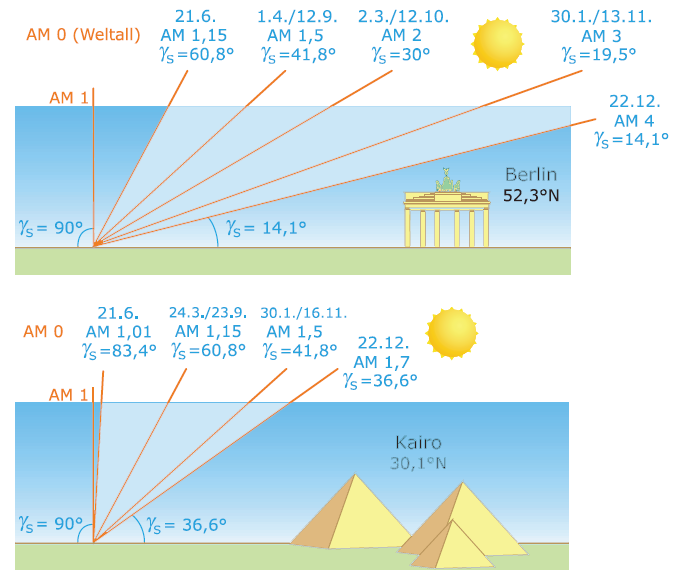
\includegraphics[width=125mm]{img/berlin.png}
\caption[Sonnenspektrum]{Vergleich des höchsten Sonnenstand und dazugehöriger AM-Werte für verschiedene Tage in Berlin und Kairo. Quelle: \cite{q01}}\label{airmass}
\end{figure}

\begin{figure}[htbp]
\centering
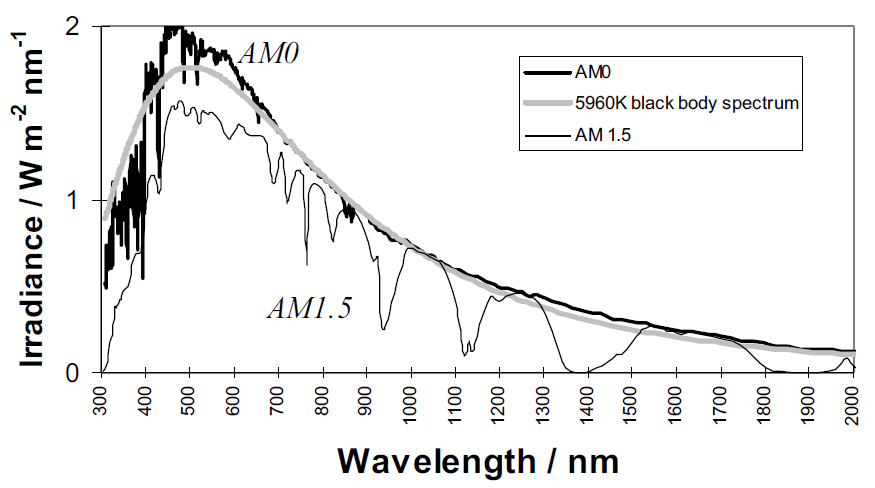
\includegraphics[width=125mm]{img/am.png}
\caption[Sonnenspektrum]{Der Vergleich von Spektrum des Sonnenlichtes im Weltall (AM0), der Strahlung eines schwarzen Körpers von 5960K und dem AM1.5 Spektrum. Quelle: \cite{n01}}\label{sunspec}
\end{figure}


\section{Sonnensimulator Aufbau}\thispagestyle{empty}


Mit der SolarConstant 4000 (siehe Abbildung \ref{sunsim}) der Firma Atlas kann die Einwirkung der Sonne auf Testobjekte simuliert werden. Dazu ist das Gerät mit zehn Metallhalogenid-Strahlungsquelle Lampen zu je 4 kW. Durch die Füllung der Lampen mit Halogeniden wird ein möglichst kontinuierliches Spektrum erzeugt. Die Leuchten sind mit Filterscheiben ausgestattet, welche das abgestrahlte Licht dem AM1.5 Spektrum annähern.
Jede Lampe wird von einem eigenen elektronisch geregelten Vorschaltgerät versorgt, welches für einen gleichmäßigen und flimmerfreien Betrieb sorgt.
Da die Lampen nicht für eine Heißzündung ausgelegt sind, wobei sie eventuell zerstört werden können, ist eine Sperrzeit von 10 Minuten zum Abkülen vorgesehen, bevor sich die Lampen wieder einschalten lassen.
Die Strahlungsleistung lässt sich reduzieren indem das gesamte Lampenfeld in die Höhe gefahren wird.
Weiters lässt sich die Bestrahlungsstärke einzelner Lampen über die Variation der elektrischen Leistung des Vorschaltgerätes variieren.
Allerdings führt eine Variation der elektrischen Leistung zu einer Änderung des Spektrums der Lampen. Aus diesem Grund wird vom Hersteller empfohlen \cite{atlas}, die Leistung der Lampen nur zwischen 80 und 100 \% zu variieren.
Die Testobjekte werden mittels Prüfgut-Einschub in einem Windkanal positioniert, dessen obere Abdeckung aus einem geeigneten Solarglas besteht. Die geneigte Glasplatte bewirkt eine Querschnittreduktion des Luftkanales und somit eine Erhöhung der Strömungsgeschwindigkeit zwischen Zuluft- und Abluftseite. Diese stetige Erhöhung der Geschwindigkeit ist notwendig, damit die sich erwärmende Zuluft eine konstante Kühlwirkung hat, um die Testobjekt auf konstanter Temperatur zu halten.


\begin{figure}[htbp]
\centering
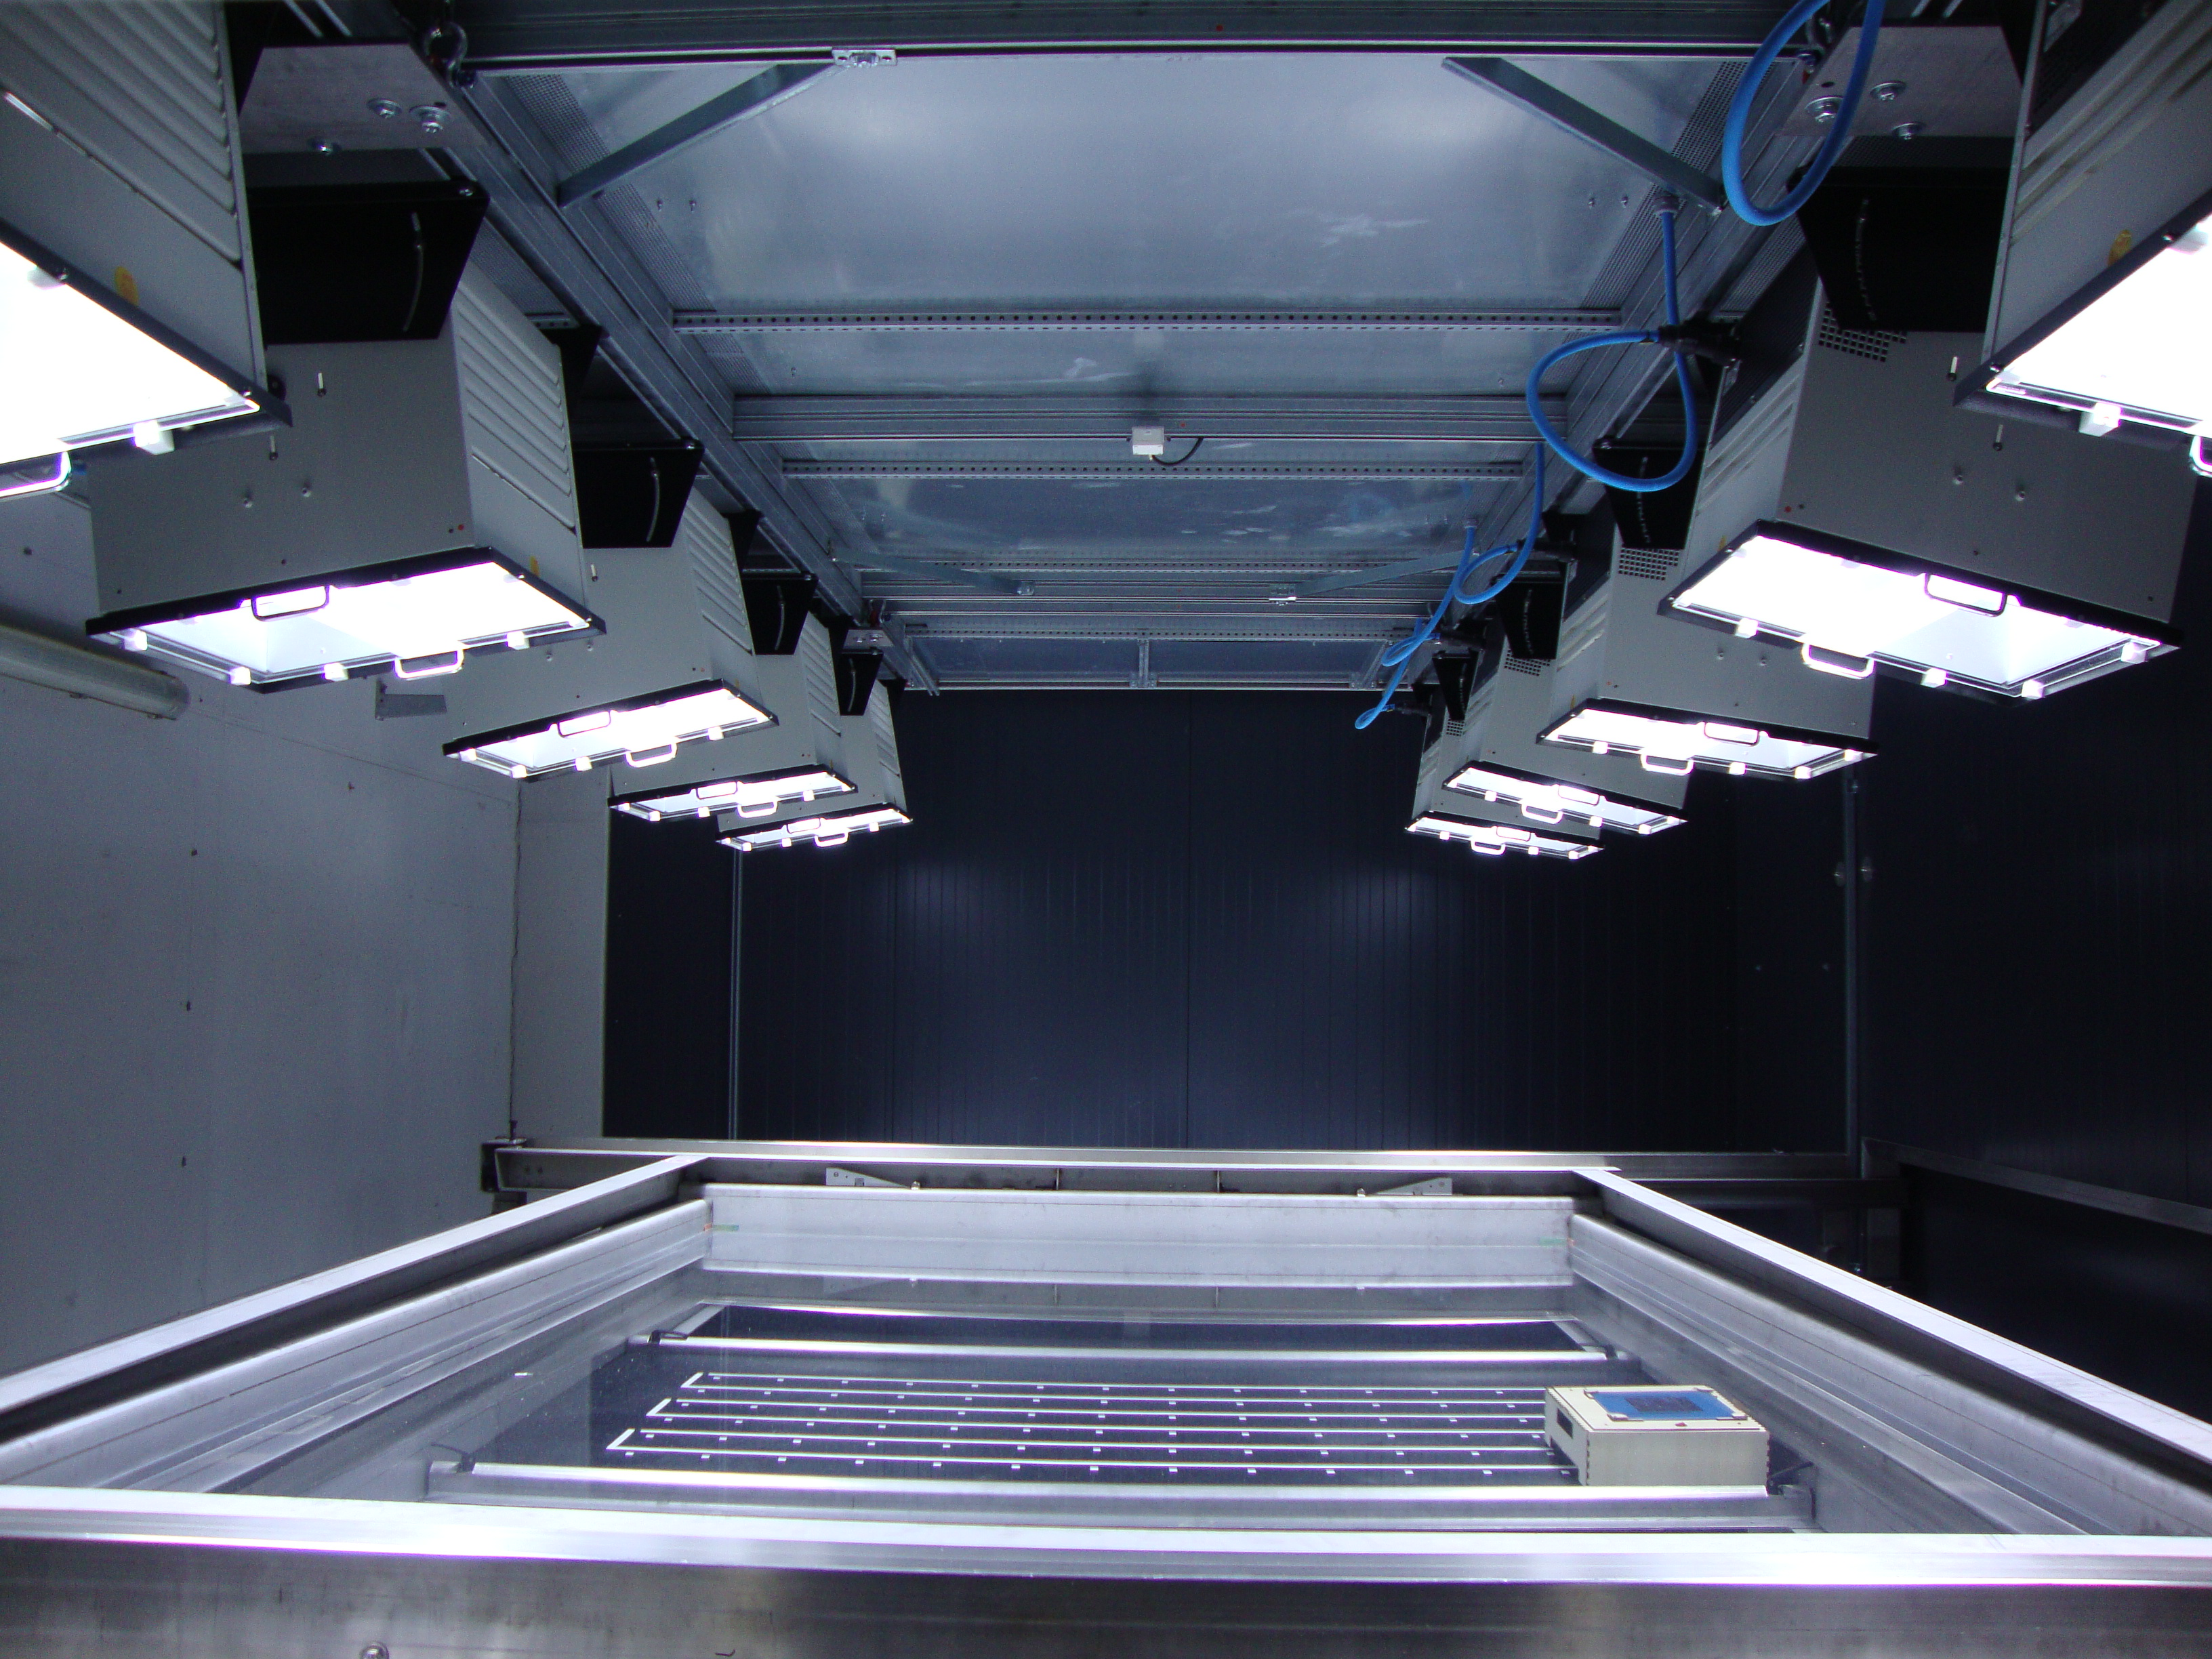
\includegraphics[width=125mm]{img/sunsimulator.jpg}
\caption[Sonnensimulator]{Der Aufbau des Sonnensimulators: Die zehn Metallhalogenoid-Strahler befestigt an der höhenverstellbaren Aufhängung, der Windkanal und die Prüfebene.}\label{sunsim}
\end{figure}


\section{Normative Anforderungen an Sonnensimulatoren}\thispagestyle{empty}
In der IEC Norm 60904-9 \cite{norm9} werden die Anforderungen an Sonnensimulatoren definiert. Ein Sonnensimulator wird anhand von 3 Kriterien bewertet: 
\begin{itemize}
\item die spektrale Übereinstimmung mit dem in Tabelle \ref{TabS1} aufgelisteten Wellenlängenbereichen. Zum AM1.5 Referenzspektrum sind durch die großen Schranken erhebliche Unterschiede möglich.
\begin{table}[htbp]
\centering
\begin{tabular}{ | c | c | c |}\hline
{\bf } & {\bf Wellenlängenbereich in nm} & {\bf \% der totalen Einstrahlung}\\ \hline
\hline
1  & 400 - 500 & 18,4 \\ \hline
2  & 500 - 600 & 19,9\\ \hline
3  & 600 - 700 & 18,4\\ \hline
4  & 700 - 800 & 14,9\\ \hline
5  & 800 - 900 & 12,5\\ \hline
6  & 900 - 1100 & 15,9\\ \hline
\end{tabular}
\caption{Spektralle Strahlungsverteilung nach IEC 60904-9}\label{TabS1}
\end{table}
\item die Gleichmäßigkeit der Bestrahlungsstärkeverteilung über die Testfläche
	\begin{equation}
 Non-uniformity (\%) = [\frac{max irradiance - min irradiance}{max irradiance + min irradiance}] \times (100\%)
\end{equation}
\item die zeitliche Stabilität der Einstrahlung.
\begin{equation}
 Temporal (\%) = [\frac{max irradiance - min irradiance}{max irradiance + min irradiance}] \times (100\%)
\end{equation}
\end{itemize}

Die Tabelle \ref{TabS2} gibt die Anforderungen an, nach denen Sonnensimulatoren in den Klassen A, B und C klassifiziert werden. Die Sonnensimulatorklasse ABB bedeutet eine 0,75- bis 1,25-fache Übereinstimmung in allen in Tabelle \ref{TabS1} angeführten Schranken, eine Homogenität der Einstrahlung zwischen 2\% und 5\% im Messbereich, und eine zeitliche Stabilität zwischen 2\% und 5\%. Der Roboter misst von diesen drei Kategorien nur die Verteilung der Bestrahlungsstärke in der Messebene.
\begin{table}[htbp]
\centering
\begin{tabular}{ | c | c | c | c | c |}\hline
\multirow{2}{*}{Klassifikation} &  Spektrale  &  Örtliche  & {Kurzzeit-}& {Langzeit-}\\
& Übereinstimmung & Homogenität & {stabilität} & {stabilität} \\ 
\hline
\hline
A  & 0,75 - 1,25 & 2 \% & 0,5 \% & 2 \%\\ \hline
B  & 0,6 - 1,4 & 5 \% & 2 \% & 5 \%\\ \hline
C  & 0,4 - 2,0 & 10 \% & 10 \% & 10 \%\\ \hline
\end{tabular}
\caption{Anforderungen an die 3 verschiedenen Simulatorklassen}\label{TabS2}
\end{table}



\section{Theorie Referenzzelle}\thispagestyle{empty}
Eine Solarzelle wandelt die Energie des Lichtes teilweise in elektrische Energie um. Eine Referenzzelle ist eine speziell für Messungen kalibrierte Solarzelle, welche als Strahlungsmessgerät dient. Wichtig ist, dass die Referenzzelle eine ähnliche spektrale Empfindlichkeit hat, wie die zu messenden Zelle bzw. das zu messende Modul.
Es gibt verschiedene Solarzellentechnologien. Es gibt kristalline Siliziumzellen und Dünnschichtzellen. Die kristallinen Siliziumzellen werden in monokristalline Zellen und multikristalline Zellen unterschieden. Beide zusammen machen über 80\% des weltweiten Photovoltaikmarktes aus \cite{iea00}. Als Referenzzelle für Messungen werden ausschließlich kristalline Zellen verwendet. 
Eine Siliziumsolarzelle ist eine großflächigen Diode (siehe Abbildung \ref{cell}). Die Sperrschicht ist dabei dem Sonnenlicht ausgesetzt. Gelangt ein Lichtquant in die Sperrschicht, kann aufgrund des inneren Photoeffektes ein Elektron/Loch Paar erzeugt werden. Durch das elektrische Feld in der Sperrschicht werden die Ladungsträger getrennt bevor sie rekombinieren können. Elektronen bewegen aufgrund ihrer negativen Ladung entgegen der Feldrichtung in die n-Zone. Löcher wandern in Feldrichtung zur raumladungsfreien p-Zone. Die Leerlaufspannung einer Solarzelle ist kleiner als die Diffusionsspannung, der Spannung über die Raumladungszone, die der Diffusion von Ladungsträgern entgegenwirkt.
\begin{figure}[htbp]
\centering
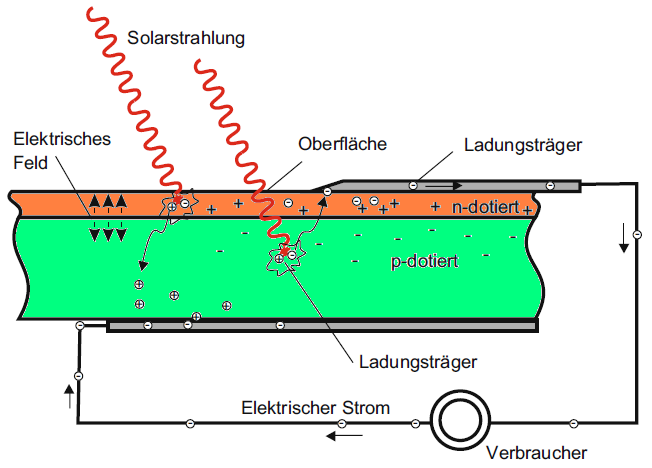
\includegraphics[width=125mm]{img/zelle2.png}
\caption{Der Schematischer Aufbau einer Siliziumsolarzelle. Quelle: \cite{pv}}\label{cell}
\end{figure}


Unbeleuchtet funktioniert die Solarzelle wie eine normale Halbleiterdiode, welche einen Durchlassstrom von p- nach n-Seite fließen lässt, falls eine Spannung von p nach n anliegt. Bei Beleuchtung wird zusätzlich ein Photostrom erzeugt, welcher proportional zur Bestrahlungsstärke und der Zellfläche ist. Das Zweidiodenmodel (siehe Abbildung \ref{esb}) besteht daher aus einer Stromquelle, dazu parallel zwei Dioden, einen Parallelwiderstand und einem Serienwiderstand. Der Parallelwiderstand fasst Kurzschlüsse zusammen, die realen Solarzellen am Rand oder an den Korngrenzen auftreten können. Mit dem Serienwiderstand werden alle Spannungsabfälle in der Solarzelle erfasst. Die beiden Dioden bilden die Rekombinations- und Diffusionsprozesse in einer realen Solarzelle ab. Eine ideale Solarzelle hat einen Serienwiderstand von null und einen Parallelwiderstand von unendlich. 
\begin{figure}[htbp]
\centering
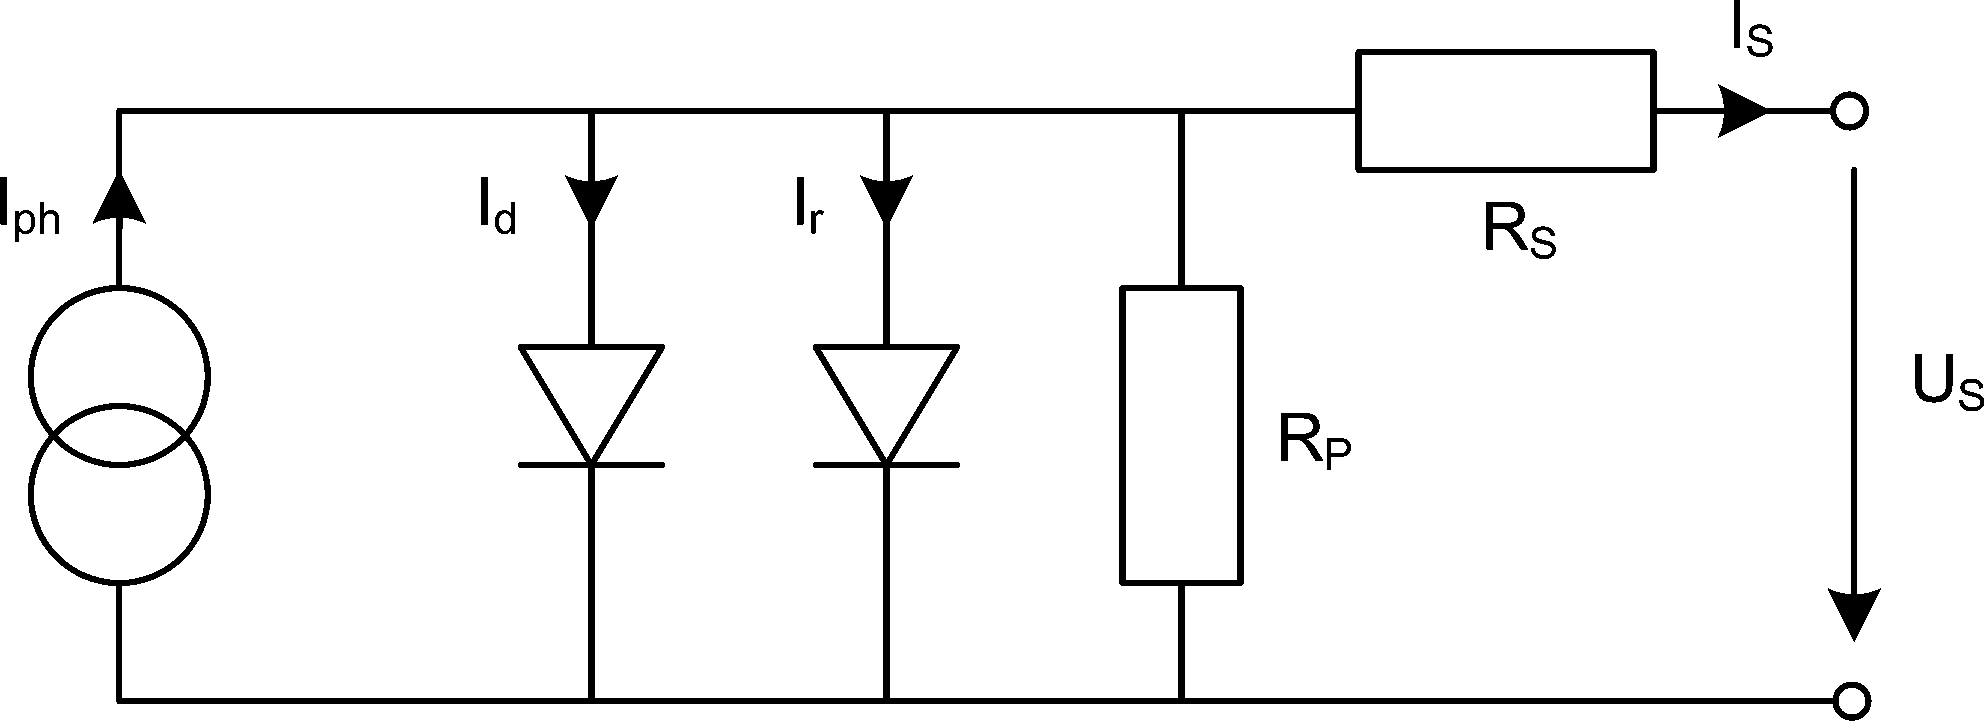
\includegraphics[width=100mm]{img/esb2.png}
\caption{Das Zweidiodenmodell einer Sorlarzelle. Quelle: \cite{pv}}\label{esb}
\end{figure}

Durch den zusätzlichen Photostrom verschiebt (siehe Abbildung ~\ref{kennlinie}) sich die Diodenkennline. Im Leerlauf  bzw. Kurzschlussbetrieb gibt die Solarzelle keine Leistung ab. Der Punkt der Kennlinie mit der maximalen Leistung wird als Maximum Power Point (MPP) bezeichnet.

Der Füllfaktor berechnet sich aus Strom im maximalen Leistungspunkt $I_{mp}$, Spannung im maximalen Leistungspunkt $U_{mp}$, Kurzschlusstrom $I_{sc}$ und Leerlaufspannung $U_{oc}$ zu:
  \begin{equation}
     FF = \frac {I_{mp} U_{mp}} {I_{sc} U_{oc}}~.
  \end{equation}
Der Füllfaktor ist das Verhältnis der Fläche des Rechteckes mit den Seitenlängen I$_{mp}$ und U$_{mp}$ zu der Fläche des Rechteckes mit den Seitenlängen I$_{sc}$ und U$_{oc}$ (siehe Abbildung \ref{kennlinie}).

\begin{figure}[htbp]
\centering
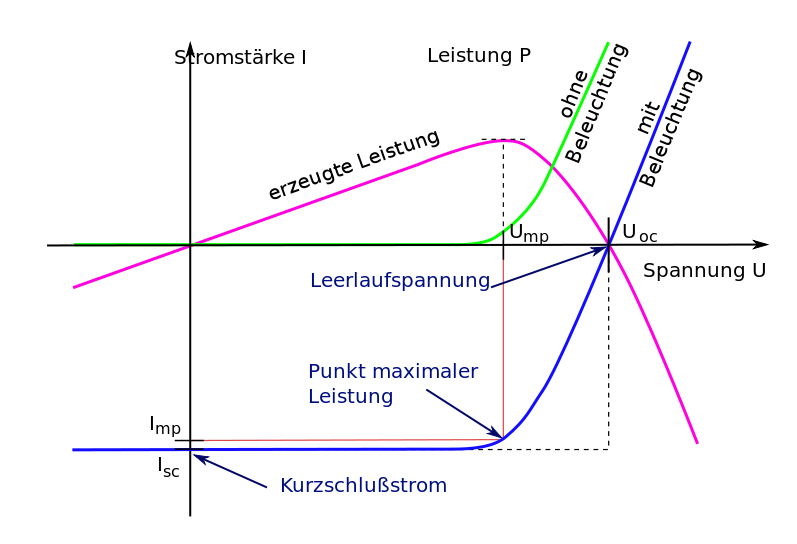
\includegraphics[width=125mm]{img/kennlinie.png}
\caption{Die Dunkel- und Hellkennlinie Eines Solarzelle. Modifiziert nach \cite{kl}}\label{kennlinie}
\end{figure}

Die Kennlinie der Solarzelle ist von der Einstrahlung abhängig (siehe Abbildung \ref{mpp}). Der Kurzschlusstrom ist direkt proportional zur Einstrahlung.
Laut IEC 60891 \cite{norm891} berechnet sich die Einstrahlung aus dem gemessenen Kurzschlussstrom, den STC-Kurzschlussstrom, einen relativen Temperaturkoeffizienten und der Zelltemperatur:
\begin{equation}
G = \frac{1000Wm^{-2}I_{RC}}{I_{RC,STC}} [1 - \alpha_{RC}(T_{RC}-25^{\circ} C]~.
\label{gg}
\end{equation}
Bei konstanter Temperatur ist der Kurzschlussstrom linear abhängig von der Bestrahlungsstärke (siehe Abbildung \ref{mpp}).
Nach der Gleichung \ref{gg} ist der Kurzschlussstrom zusätzlich von der Temperatur anhängig, daher ist es notwendig die Temperatur der Zelle zum Zeitpunkt der Messung zu ermitteln, sowie den Temperaturkoeffizienten $\alpha_{RC}$ zu kennen.
\begin{figure}[htbp]
\centering
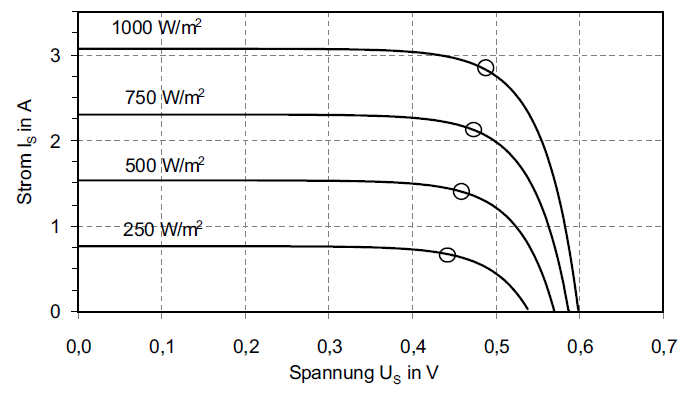
\includegraphics[width=125mm]{img/kennlinien.png}
\caption{Die lineare Abhängigkeit des Kurzschlussstromes von der Einstrahlung. Quelle: \cite{pv}}\label{mpp}
\end{figure}

In der Abbildung \ref{el} ist ein Elektrolumineszenz-Aufnahme der verwendeten Messzelle zu sehen. Es ist deutlich die multikristalline Struktur der Zelle zu erkennen. 

\begin{figure}[htbp]
\centering
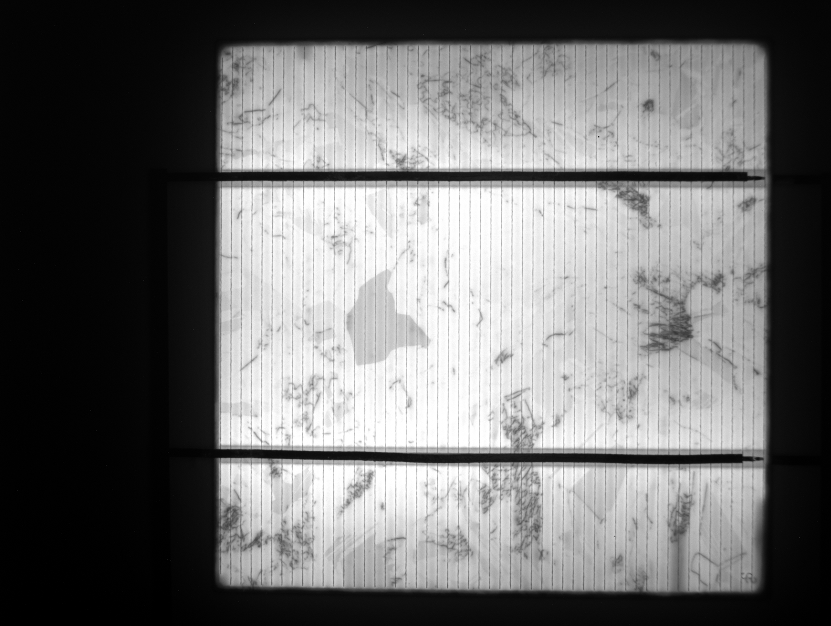
\includegraphics[width=100mm]{img/el.png}
\caption{Eine EL-Aufnahme der verwendeten Messzelle.}\label{el}
\end{figure}

\chapter{Entwicklungsprozess}\thispagestyle{empty}

Diese Kapitel beschreibt die Entwicklung des Roboters und ist in drei Abschnitte gegliedert: das mechanische Design, die Elektronik sowie die Steuerungs- und Messsoftware.
Die Entwicklung der Software und der Hardware geschah zum Teil parallel. Zur Entwicklung der Fahrregelung musste die Bodenplatte, aber nicht der Aufbau des Chassis fertig sein. Ebenso reichte ein Teil der Elektronik aus, die Messplatinen und die endgültige Stromversorgung war zur Entwicklung der Fahrregelung nicht notwendig. Das hatte den Nachteil, dass die Größe mancher Komponenten (z.B. der Akku) nur abgeschätzt werden konnte, und der Roboter nicht auf eine minimale Größe hin optimiert wurde.

\section{Mechanische Komponenten}\thispagestyle{empty}

Dieser Abschnitt behandelt die Entwicklung der mechanischen Komponenten. Diese sind die vier Mecanumräder und das Chassis des Roboters. Die maximale Bauhöhe ist durch den Windkanal im Sonnensimulator beschränkt, die minimale Bauhöhe ist durch den Durchmesser der Räder gegeben.
Mit der Größe der Messzelle ist auch die minimale Ausdehnung in den beiden anderen Dimensionen festgelegt. Eine weiter Einschränkung beim Design war, dass die Motoren, der Akku und die Elektronik im Inneren des Roboters Platz finden mussten, wodurch der Roboter länger und breiter als die Messzelle wurde (siehe Abbildung \ref{oben}). In dem Bild des Roboters sind die Messzelle, sowie der Einschalter und der Programmwahlschalter zu erkennen.

\begin{figure}[htbp]
\centering
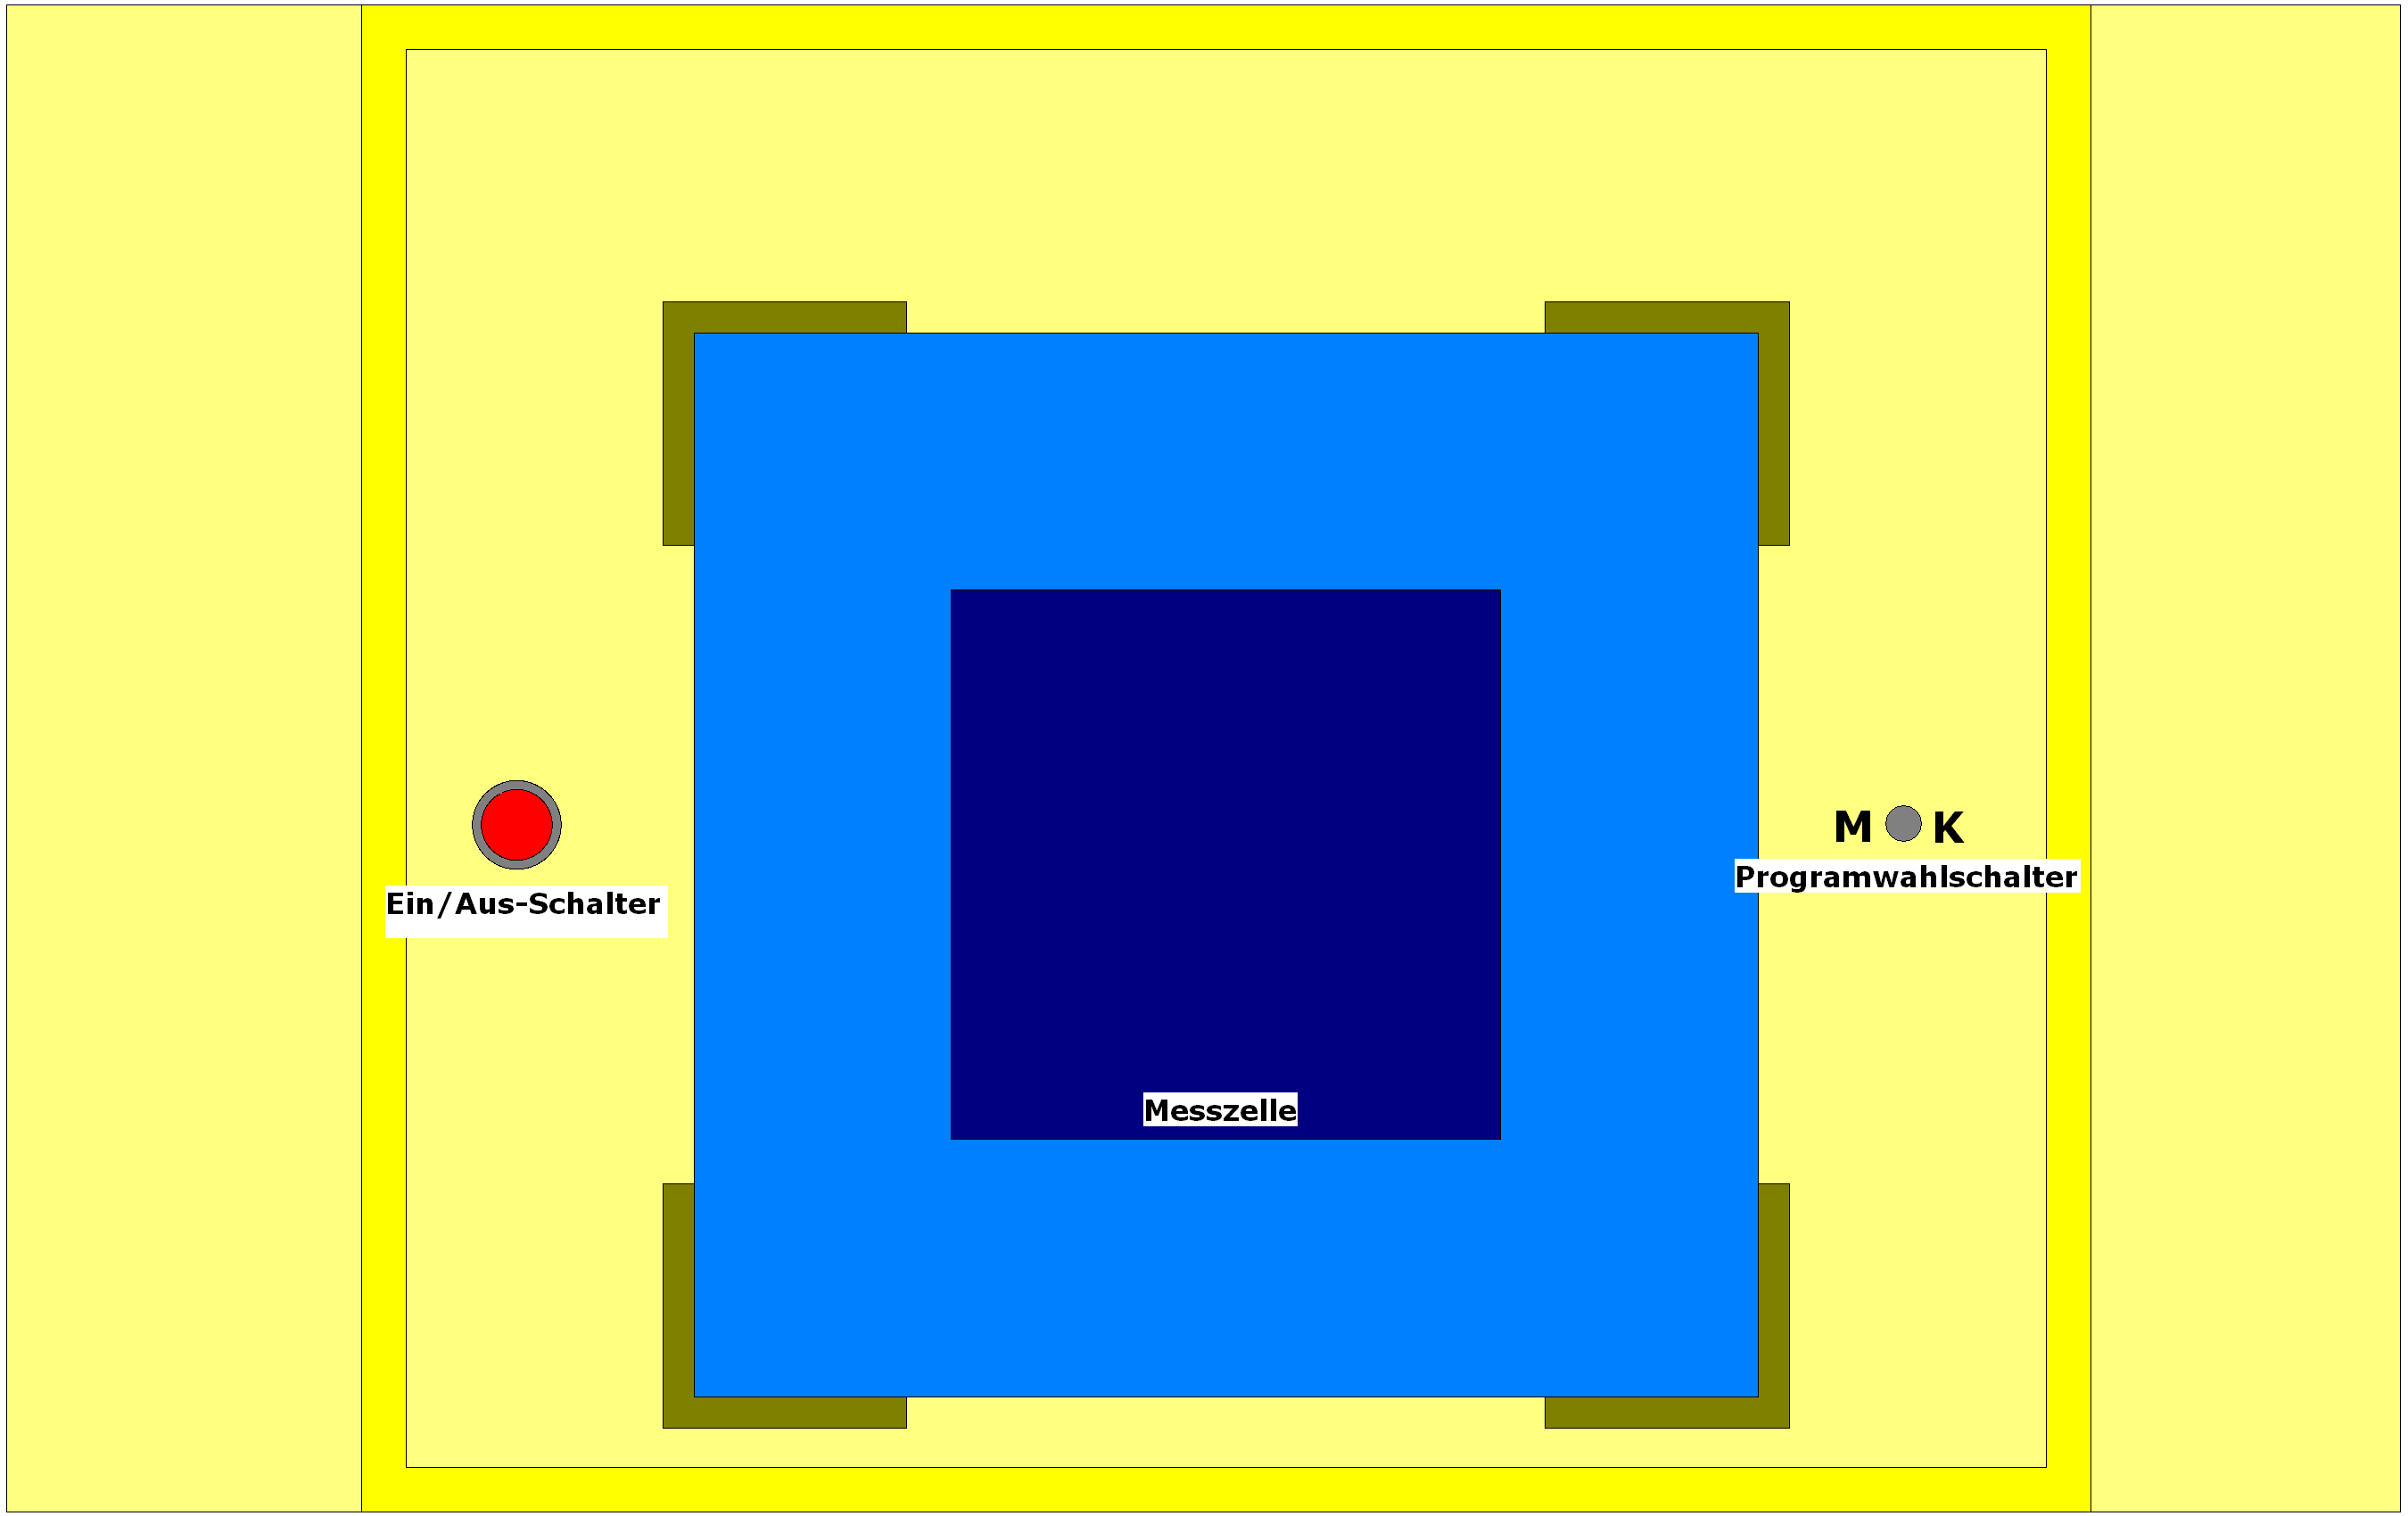
\includegraphics[width=125mm]{img/oben3.png}
\caption{Der Roboter aus der Vogelperspektive.}\label{oben}
\end{figure}
  

\subsection{Die Mecanum-Plattform}\thispagestyle{empty}
Mecanum-Räder erlauben einem Fahrzeug ohne mechanischer Lenkung, sich in jede Richtung zu bewegen. Benannt ist es nach dem schwedischen Unternehmen Macanum, welches dieses Rad 1971 entwickelt hat \cite{mecanum}. 
Jedes Rad wird mit einem eigenen Motor angetrieben, und verfügt über eine separate Ansteuerung. Die Räder bestehen aus einer Felge (siehe Abbbildung \ref{rad}), auf der unter einem Winkel von 45 Grad befestigte, ballige Rollen so angebracht sind, die über den Abrollumfang einen Kreis bilden (siehe Abbbildung \ref{rad2}). In die 8 Löcher der Felge werden Kugellager eingeklebt. Jedes der vier Räder besteht aus einer Felge, insgesamt 16 Laufrollen, 8 Kugellager, 8 M4x45mm Schraube, 8 M4-Muttern, sowie 16 M4-Beilagscheiben. 
Das Rad ist mit einer M3-Schraube und einer M3-Mutter an der Motorachse fixiert.
Die Felgen und die Laufrollen wurden mit einem Ultimaker 3D-Drucker [\cite{um})gedruckt. 
Die Vorlage namens "Mecanum Wheel MK2" stammt von http://www.thingiverse.com/thing:2473, und kann unter der Attribution-NonCommercial-ShareAlike 3.0 Unported Lizenz nicht-kommerziell verwendet werden.
Die Laufrollen wurden modifiziert, so dass die Mutter sowie der Schraubenkopf in der Rolle versenkt sind, damit das Rad insgesamt kompakter ist. Zum Bearbeiten wurde OpenSCAD, ein 3D-Compiler, verwendet. 

Durch die Schräganordnung der Laufrollen entstehen beim Antreiben eines Rades zwei Kraftkomponenten, eine in Querrichtung sowie eine in Längsrichtung des Fahrzeuges. Gegeneinander gerichtete Kräfte der einzelnen Räder werden über die Achsen und den Rahmen kompensiert. Die übrigen Kräfte addieren sich zur resultierenden Fahrtrichtung. Auf diese Weise sind durch entsprechendes Ansteuern der einzelnen Räder omnidirektionale Fahrmanöver möglich (siehe Abbildung \ref{fahrman}). So ist es nicht nur möglich den Roboter in Längsrichtung vor und zurück zu bewegen, sondern auch in Querrichtung (normal zur Längsrichtung) zu bewegen, ebenso sind Drehungen am Stand möglich. Damit braucht ein mit Mecanumrädern ausgestatteter Roboter keine Lenkung. Allerdings sind vier Motoren notwendig, damit jedes Rad einzeln angesteuert werden kann.   
Die Kugellager sind in den acht passenden Löchern der Felge verklebt, zuerst mit einem handelsüblichen Sekundenkleber, allerdings haben sich einige Kugellager im Laufe der Zeit gelöst und beeinflussten so das Fahrverhalten negativ, danach mit einem Zweikomponentenkleber. Eine dauerhafte Verbindung von Kugellager mit der Felge ist für den störungsfreien Betrieb des Roboters unumgänglich. 
Zwischen den Rollen und dem Kugellager sorgen Beilagscheiben für einen reibungsarmen Betrieb. 
Die Schrauben der Rollen lösen sich im Betrieb nicht. Die Schraube, welche die Felge an der Motorachse befestig hat, löste sich regelmäßig, bis diese Verbindung mit einem Kleber gesichert wurde.
An den Rollen ist keine Abnützung erkennbar. Einige Halterungen der Kugellager brachen schon während der Erstmontage, verschlimmert hat sich während der Betriebes nichts.
Es wurde lange mit teilweise defekten Rädern gefahren, ein Messbetrieb war aber dennoch möglich. Insgesamt ist die Mecanum-Plattform eine robuste Lösung für Messroboter.
Die Kugellager sind wartungsfrei. Das wenige UV-Licht, das den PLA-Kunststoff erreicht hat auch nach Monaten noch keine negativen Auswirkungen auf die mechanischen Eigenschaften der Räder.

\begin{figure}
    \subfigure[Vor/Zurück-Fahren]{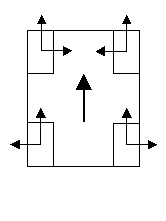
\includegraphics[width=50mm]{img/gerade.png}}
    \subfigure[Das Seitwärtsfahren]{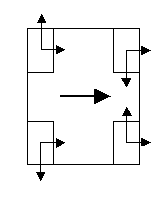
\includegraphics[width=50mm]{img/seitw.png}}
     \subfigure[Drehen am Stand]{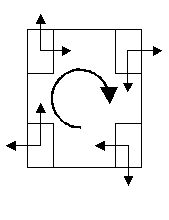
\includegraphics[width=50mm]{img/dreh.png}}
\caption{Einige der möglichen Fahrmanöver eines Mecanum-Rad-Fahrzeuges.}\label{fahrman}
\end{figure} 

\begin{figure}[htbp]
\centering
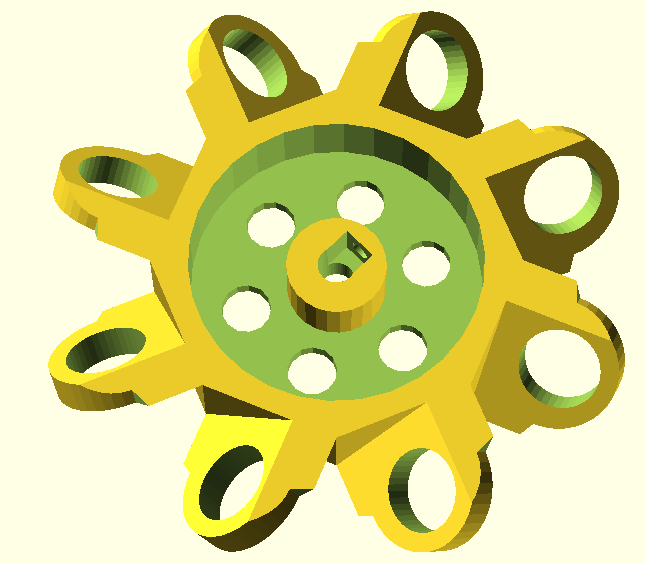
\includegraphics[width=75mm]{img/wheel.png}
\caption{Die Felge eines Mecanum Rades.}\label{rad}
\end{figure}

\begin{figure}[htbp]
\centering
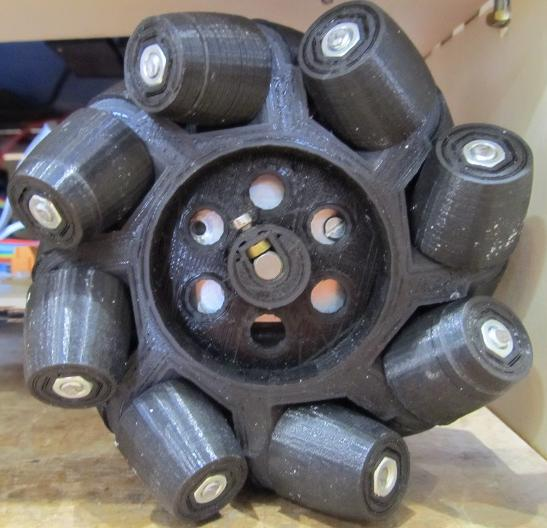
\includegraphics[width=75mm]{img/rad.jpg}
\caption{Ein komplettes Rad, montiert am Roboter.}\label{rad2}
\end{figure}


Mit OpenSCAD entsteht ein dreidimensionales Modell eines Werkstückes. Damit fängt ein 3D-Drucker nichts an. Ein 3D-Druck setzt sich aus sehr vielen Liniensegmenten zusammen. Dazu muss das 3D-Modell in einzelne dünne Schichten und einzelne Linien zerlegt werden. Dieser Vorgang wird als "Slicing" bezeichnet. Dazu wurde das Programm Skeinforge verwendet. Mit OpenSCAD wird zunächst ein stl-File erzeugt, dann produziert Skeinforge daraus die Fahrbefehle für den 3D-Drucker in Form eines G-Code. Als Druckmaterial wurde PLA (polylactic acid) verwendet, welches in einem Temperaturbereich von 215 bis 230 Grad Celsius per Extruder verarbeitet werden kann.    
Die Druckzeit pro Rolle betrug 20 Minuten. Insgesamt mussten 64 Rollen gefertigt werden. Die Druckzeit pro Felge betrug etwa drei Stunden, der Roboter benötigte vier Felgen. Es gibt zwei verschiedene Felgentypen, mit nach links oder nach rechts geneigten Rollen. 
Die Zeitaufwand wurde durch vorbereitende Testdrucke, bis die einzelnen Komponenten optimiert waren und der Drucker befriedigend Ergebnisse lieferte, sowie Fehldrücke, zusätzlich verlängert. 
Nach dem Drucken mussten die Teile nachbearbeitet werden. Die Löcher für die Kugellager mussten per Hand passend gefeilt werden. Beim  Einsetzen der Kugellager brachen zwar manche der Halterungen, aber mit Klebstoff konnten die Kugellager auch in die gebrochenen Halterungen fixiert werden. Die dauerhafte Haltbarkeit dieser Klebungen war allerdings anfangs mit einem Fragezeichen behaftet. Die erste Klebung der Kugellager hat den Testalltag nicht überstanden. Trotz loser Kugellager konnte der Roboter dennoch erfolgreich Messfahrten durchführen. Mit einem Zweikomponentenkleber wurden die Kugellager ein zweites Mal, diesmal dauerhaft, eingeklebt.

\subsection{Chassis}\thispagestyle{empty}

\noindent Das Chassis wurde aus Sperrholz gefertigt. Dieses Material wurde gewählt weil es leicht zu bearbeiten, robust und UV-beständig ist. Das Design wurde mit QCAD [\ref{qm}] entwickelt. QCAD ist ein 2-dimensionales CAD Programm. 
Die Abmessungen des Chassis wurde im Wesentlichen abgestimmt auf: \begin{itemize}
\item Den Durchmesser und der Breite der Mecanum Räder, die innerhalb des Chasis liegen, damit die Räder vor der UV Strahlung geschützt sind, kein Einfluss (Beschattung oder Reflexionen) auf die Messzelle besteht.
\item Die Größe der Motoren.
\item Den Arduino-Mikrocontroller , die Motorsteuerelektronik und die Messelektronik.
\item Den Akku zur Stromversorgung, die dazugehörende Akku Spannungsüberwachung.
\item Die Abmessung der eingekapselten Solarzelle.
 \end{itemize}

Das Chassis besteht aus der Bodenplatte, den Seitenwänden und der oberen Abdeckung mit der Aufnahme für die Messzelle (siehe Abbildung \ref{gehause}). In der Bodenplatte sind Bohrlöcher zur Befestigung der Motoren und für die Montage der Sensorarrayplatine an der Unterseite vorhanden. Zusätzlich gibt es zwei rechteckige Löcher für die Verbindungskabel zur Sensorarrayplatine. Die beiden Seitenwände sind zur Verringerung des Luftwiderstandes geneigt (siehe Abbildung \ref{robo3d}). (Und um dem Roboter den Look eines Schuhkartons zu nehmen.)
\noindent Die Einzelteile wurden mit einem Lasercutter aus einer Sperrholzplatte geschnitten. Damit eine zukünftige Wartung problemlos möglich ist, wurde der Aufbau verschraubt ausgeführt. 
Die Motoren sind an die Bodenplatte angeschraubt, damit ein Austausch möglich ist. Auch die einzelnen Räder, wie auch die Rollen lassen sich bei Bedarf austauschen. 
Die Messzelle ist am Roboter oben befestigt.


\begin{figure}[htbp]
\centering
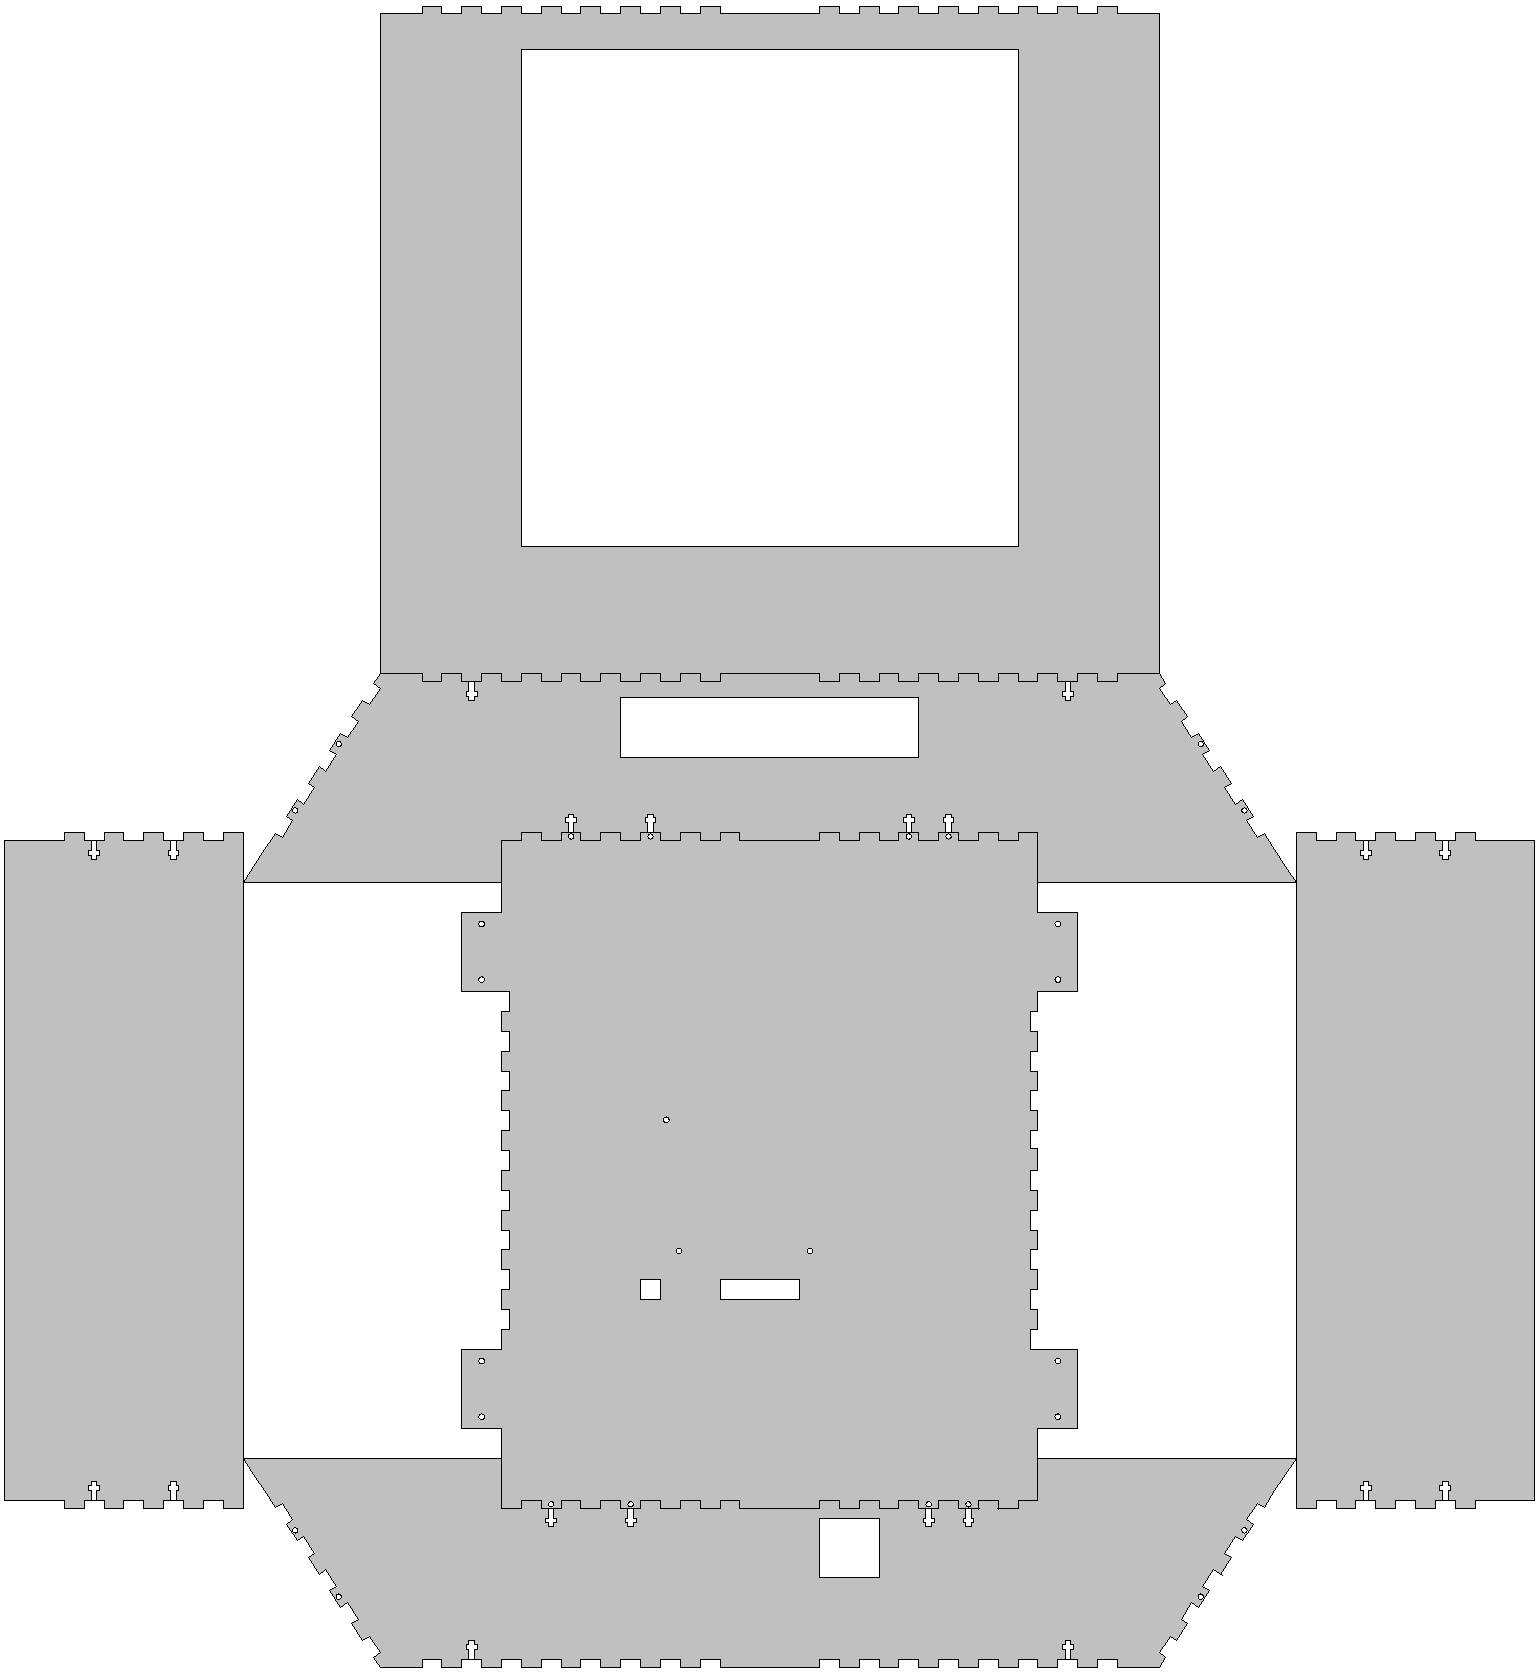
\includegraphics[width=125mm]{img/gehause3.png}
\caption[Chassis]{Die Schnittvorlage des Chassis.}\label{gehause}
\end{figure}

\begin{figure}[htbp]
\centering
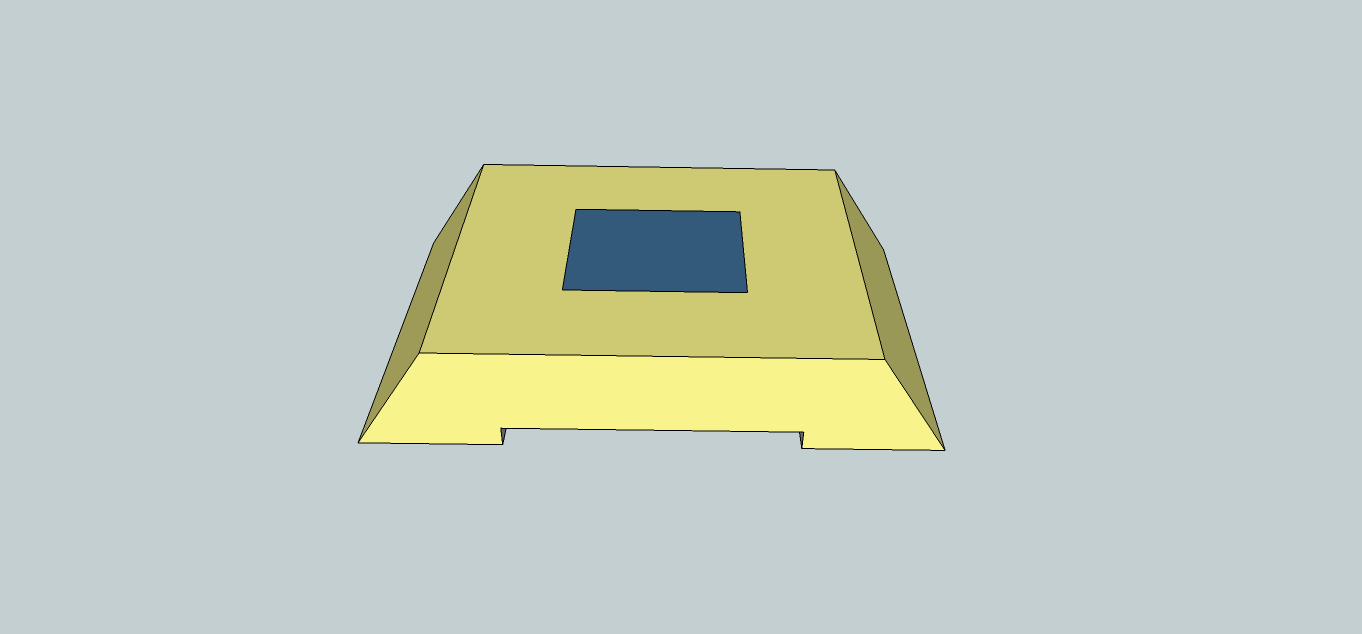
\includegraphics[width=125mm]{img/robo3d.png}
\caption[Chassis]{Ein 3D-Modell des Chassis.}\label{robo3d}
\end{figure}


\section{Elektronik}\thispagestyle{empty}

Dieser Abschnitt beschreibt die Entwicklung der Elektronik. Die Funktionalität wurde auf verschiedene Module aufgeteilt. Das erleichterte die Platzierung der Elektronik innerhalb des Messroboters, die parallele Entwicklung von Elektronik und Software, sowie den Austausch von Komponenten im Fehlerfall. 
Der Mikrocontroller des Roboters ist Teil des Arduino Mega 2560 Boards. Darauf aufgesteckt ist ein sogenanntes Shield, eine selbst entwickelte Platine, die die $\pm$5V Spannungsversorgung, die Schnittstellen zu den anderen Platinen und einen SD-Karten Einschub beheimatet.
Es gibt drei Messplatinen, eine für den Kurzschlussstrom der Messzelle, zwei für Temperaturmessungen. Eine Platine überwacht den Ladezustand des Akkus. Die Steuerung der vier Motoren ist auf einer Platine zusammengefasst.
Die einzelnen Komponenten sind wie in Abbildung \ref{elek} auf der Bodenplatte angeordnet.
Die horizontale Anordnung ist in Abbildung \ref{vorne} zu erkennen: Das Sensorarray zur Erkennung der Bodenmarkierungen ist unterhalb der Bodenplatte befestigt. Auf der Bodenplatte findet die restliche Elektronik und die Motoren Platz, die Messzelle ist auf der Oberseite des Messroboters angebracht.
Die Platinen wurden mit Eagle entwickelt. Die Platinen wurden nicht geätzt, sondern mit einer Platinenfräse gefertigt, was die eigenwillige Anordnung der Leiterbahnen erklärt. 
\begin{figure}[htbp]
\centering
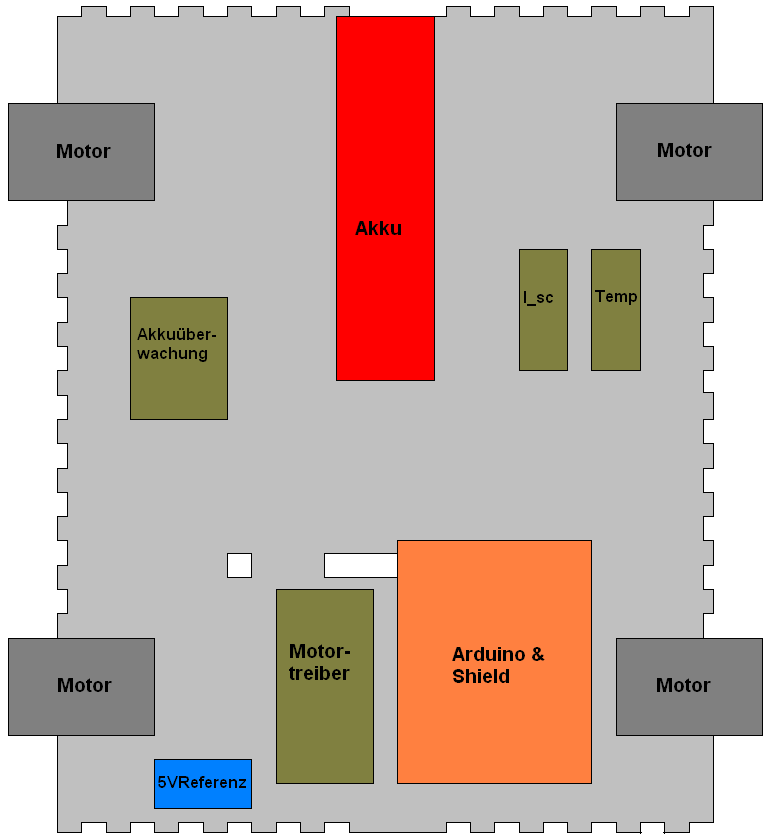
\includegraphics[width=100mm]{img/bodenplatte.png}
\caption{Die Anordnung der Elektronik auf der Bodenplatte im Roboter.}\label{elek}
\end{figure}
 
\begin{figure}[htbp]
\centering
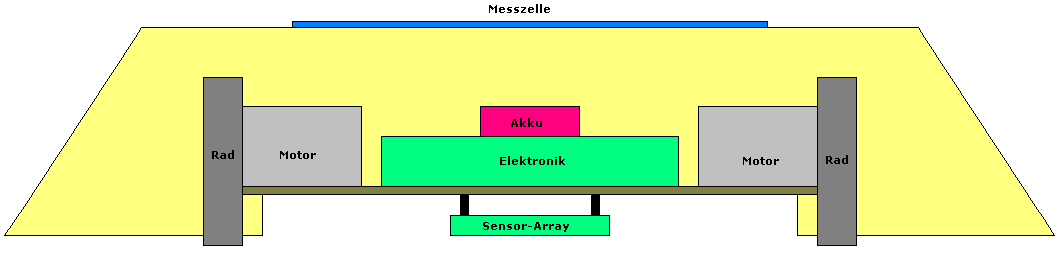
\includegraphics[width=150mm]{img/vorne.png}
\caption{Die horizontale Anordnung der Elektronik im Roboter.}\label{vorne}
\end{figure}

\FloatBarrier
 
\subsection{Motorensteuerung}\thispagestyle{empty}

Die Motorplatine besteht aus zwei integrierten H-Brücken-Bausteinen (IC1, IC2), einer 16 poligen Buchse und fünf zweipoligen Buchsen für die Stromversorgung und den Anschluss der vier Motoren. Bei den integrierten H-Brücken-Baustein handelt es sich um einen NJM2670 \cite{njm}, welcher zwei H-Brücken in einem Baustein vereint, zusätzlich verfügen diese Bausteine über eine interne Logik, welche Kurzschlüsse über die Brücke unmöglich macht.
Die Drehzahl der Motoren wird mit Pulsweitenmodulation variiert. Die PWM-Ausgänge des Arduino arbeiten mit einer Frequenz von etwa 500Hz \cite{pwm}, was den Transistoren der Brücke keinerlei Probleme bereitet.
Die Gleichspannungsmotoren sind Getriebemotoren mit der Bezeichnung RB 35, und einem Übersetzungsverhältnis von 1:200. Die maximale Versorgungsspannung wurde mit 12V angegeben. Die Leerlaufdrehzahl beträgt bei einer Versorgungsspannung von 12V 20 Umdrehungen pro Minute.
Der Roboter wird mit einem Lithium-Ionen-Akku versorgt. Die Spannung beträgt, abhängig vom Ladezustand zwischen 16,4V und 15,0V. Damit die 12V-Motoren nicht überlastet werden, wird bei der Pulsweitenmodulation ein maximales Tastverhältnis von 50\% eingehalten.

\begin{figure}[htbp]
\centering
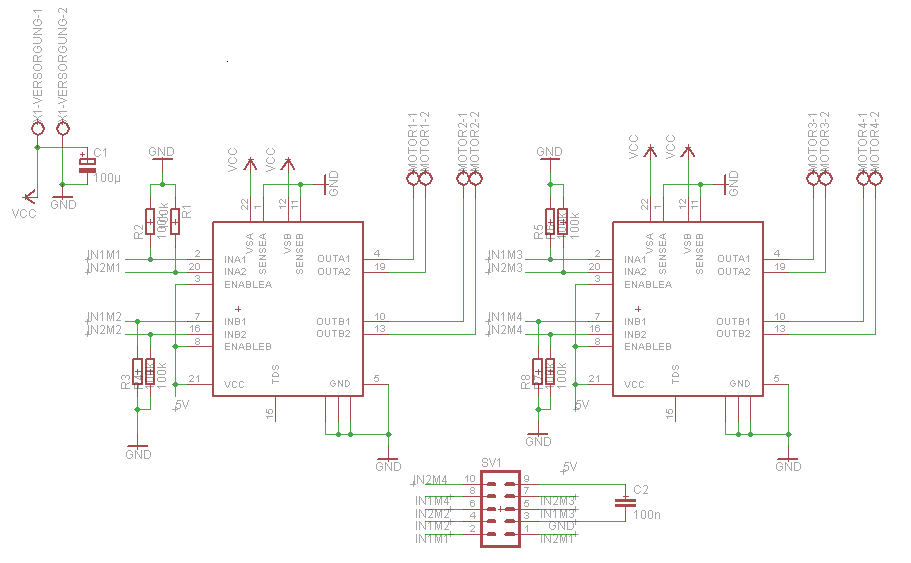
\includegraphics[width=150mm]{img/HBrucke.png}
\caption{Der Schaltplan der Motortreiberplatine.}\label{hbridge1}
\end{figure}

\begin{figure}[htbp]
\centering
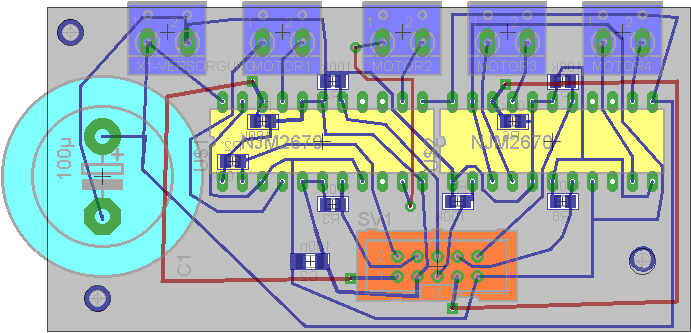
\includegraphics[width=100mm]{img/hdrive.png}
\caption{Das Layout der Motortreiberplatine.}\label{hbridge2}
\end{figure}

\FloatBarrier

\subsection{Optische Sensoren}\thispagestyle{empty}
Die optische Sensorik dient der Positionsbestimmung. Der Roboter bewegt sich während der Messung auf Holzplatten, die aus Gründen, welche unten genauer erläutert werden, schwarz sind. Der Roboter orientiert sich an einer aus geraden Teilstücken bestehenden weißen Linienfolge. 
Als Sensor wurde ein CNY70 \cite{cny} verwendet. Der CNY 70 ist ein Reflexionssensor, bestehend aus einer Infrarot-LED und einem Phototransistor in einem kompakten 7x7x6 Millimeter Gehäuse. Die LED sendet Infrarotlicht mit einem Maximum bei 950nm aus, welches an einer nahen Fläche reflektiert wird, und den Phototransistor ansteuert (siehe Abbildung \ref{cny}). Der Phototransistor verfügt über einen Tageslichtfilter. Damit können Unterschiede des Reflektionskoeffizienten gemessen werden. Das Messprinzip funktioniert bei einem Abstand von wenigen Millimetern.  Die Mess-Markierungen sind weiß auf schwarzen Untergrund ausgeführt, um gut unterscheidbare Messwerte zu bekommen. Eine Anordnung von neun solcher Sensoren in einem drei-mal-drei Array kann sowohl vertikale als auch horizontale Linien sowie Ecken erkennen. Zusätzlich gibt es einen zehnten Sensor, der die Stopmarkierungen für die Messungen erkennt.
Die neun Sensoren sind im Rastermaß 15,2 mm (= 0,6 Zoll) angeordnet. Der Stopsensor hat einen Abstand von 40,6 mm (= 1,6 Zoll) zu dem Sensorarray. 
Der Strom durch die LEDs ist mittels Potentiometer einstellbar. 
Die Platine ist zweiseitig ausgeführt, allerdings sind bis auf die OPVs in SMD-Ausführung alle Bauteile an der Unterseite der Platine montiert. Das ursprüngliche Layout wurde um folgende zwei Änderungen modifiziert:
\begin{itemize}
\item Auf die Steuerleitung des Transistors wurde vergessen. Da es noch freie Pins am 16-poligen Stecker gab, wurde diese Verbindung mittels Draht hergestellt.
\item Die Platine wird mit der 5 Volt Versorgung der restlichen Elektronik versorgt, um Probleme mit zwei verschiedenen 5 Volt Versorgungen zu vermeiden. Dazu wurde der ursprünglich vorgesehene 7805 ausgebaut, und eine weiterer freier Pin des 16-poligen Steckers verwendet.
\end{itemize}

\begin{figure}
\centering
    \subfigure[Gehäuse und Innenleben]{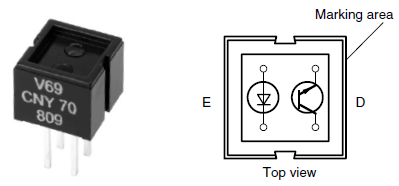
\includegraphics[width=0.4\textwidth]{img/cny1.png}}
    \subfigure[Funktion]{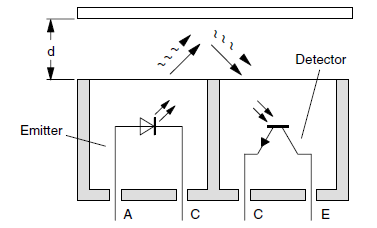
\includegraphics[width=0.4\textwidth]{img/cny2.png}}
\caption{Der Bauteil CNY70.} \label{cny}
\end{figure} 

\begin{figure}[htbp]
\centering
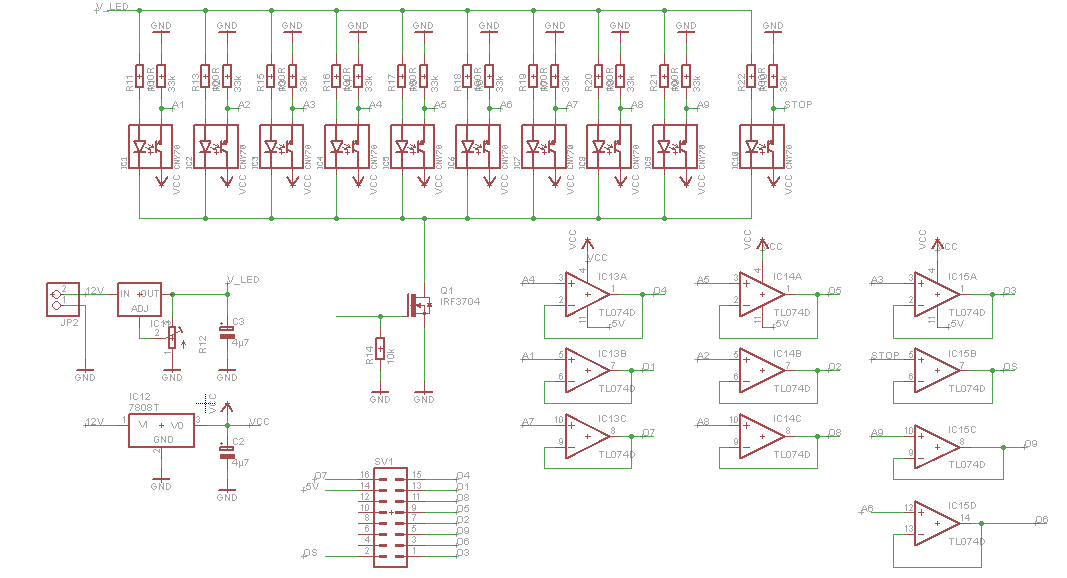
\includegraphics[width=125mm]{img/array.png}
\caption{Der Schaltplan des Sensorarrays.}\label{array}
\end{figure}

Die LEDs sind parallel geschaltet und werden alle über den Feldeffekttransistor IRF530 \cite{irf} geschaltet.
Der Strom durch die LEDs wird mit einem LM317 geregelt. Da der Widerstand als Potentiometer ausgeführt ist, lässt sich der Strom einstellen. Trotz einer nicht konstanten Versorgungsspannung kann so einer konstanter Strom geliefert werden. Um das analoge Messsignal der Phototransistoren nicht zu belasten, werden die analogen Photosignale über einen Spannungsfolger geführt. Die OPVs benötigen allerdings eine symmetrische Versorgung mit $\pm$5 V. Beide Spannungen werden über den Stecker geliefert.
Es gibt weiteren Stecker mit zwei Pins, welche die Spannungsversorgung mit 16 Volt und GND sicherstellt. 
Die Platine verfügt um drei Bohrlöcher mit jeweils drei Millimeter Durchmesser zu Befestigung.
Es ist eine 16-polige Leiterplattenbuchse für die zehn Analogsignale, die 5V-Versorgung, und des Digitalsignal zum Schalten des FET vorhanden. Des Weiteren ist ein zweipoliger Stiftstecker für die Stromversorgung mit der Akkuspannung vorhanden.

\begin{figure}[htbp]
\centering
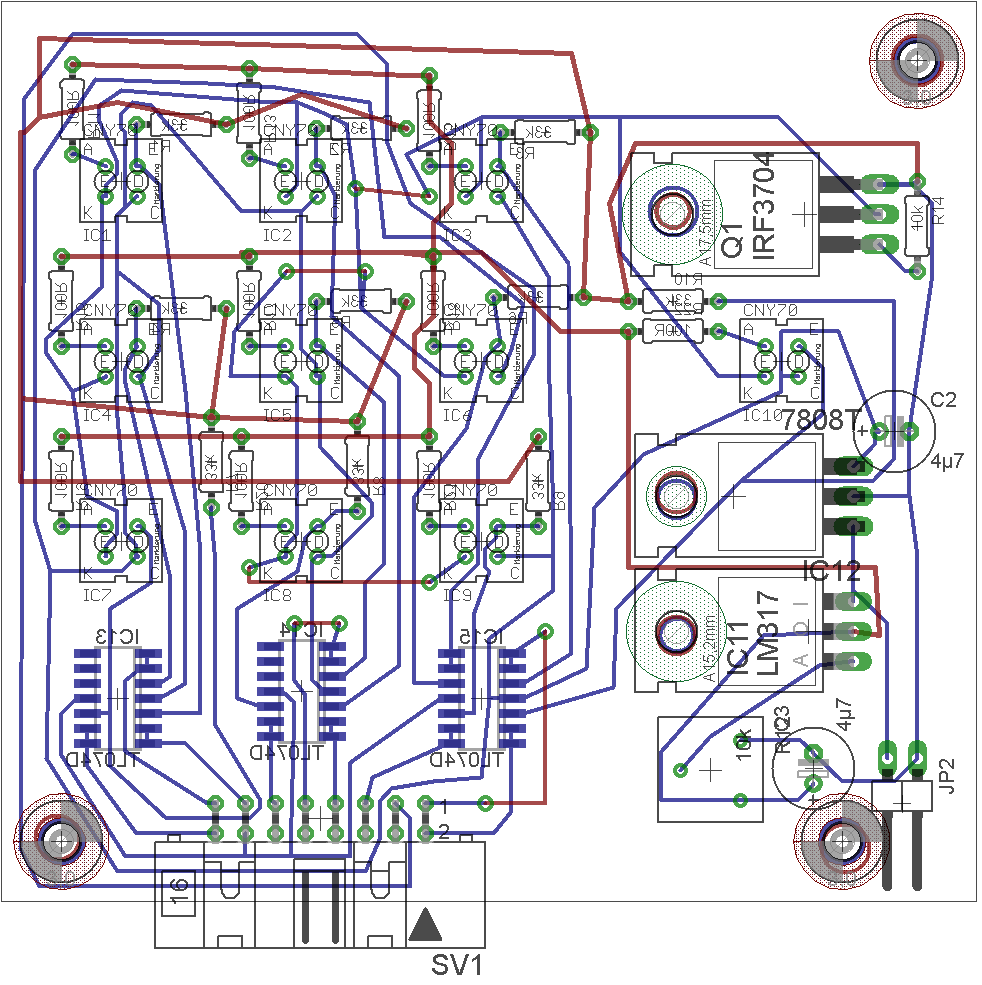
\includegraphics[width=100mm]{img/array21.png}
\caption{Das Layout des Sensorarrays. Die optischen Sensoren sind rosa markiert.}\label{array2}
\end{figure}

\begin{figure}[htbp]
\centering
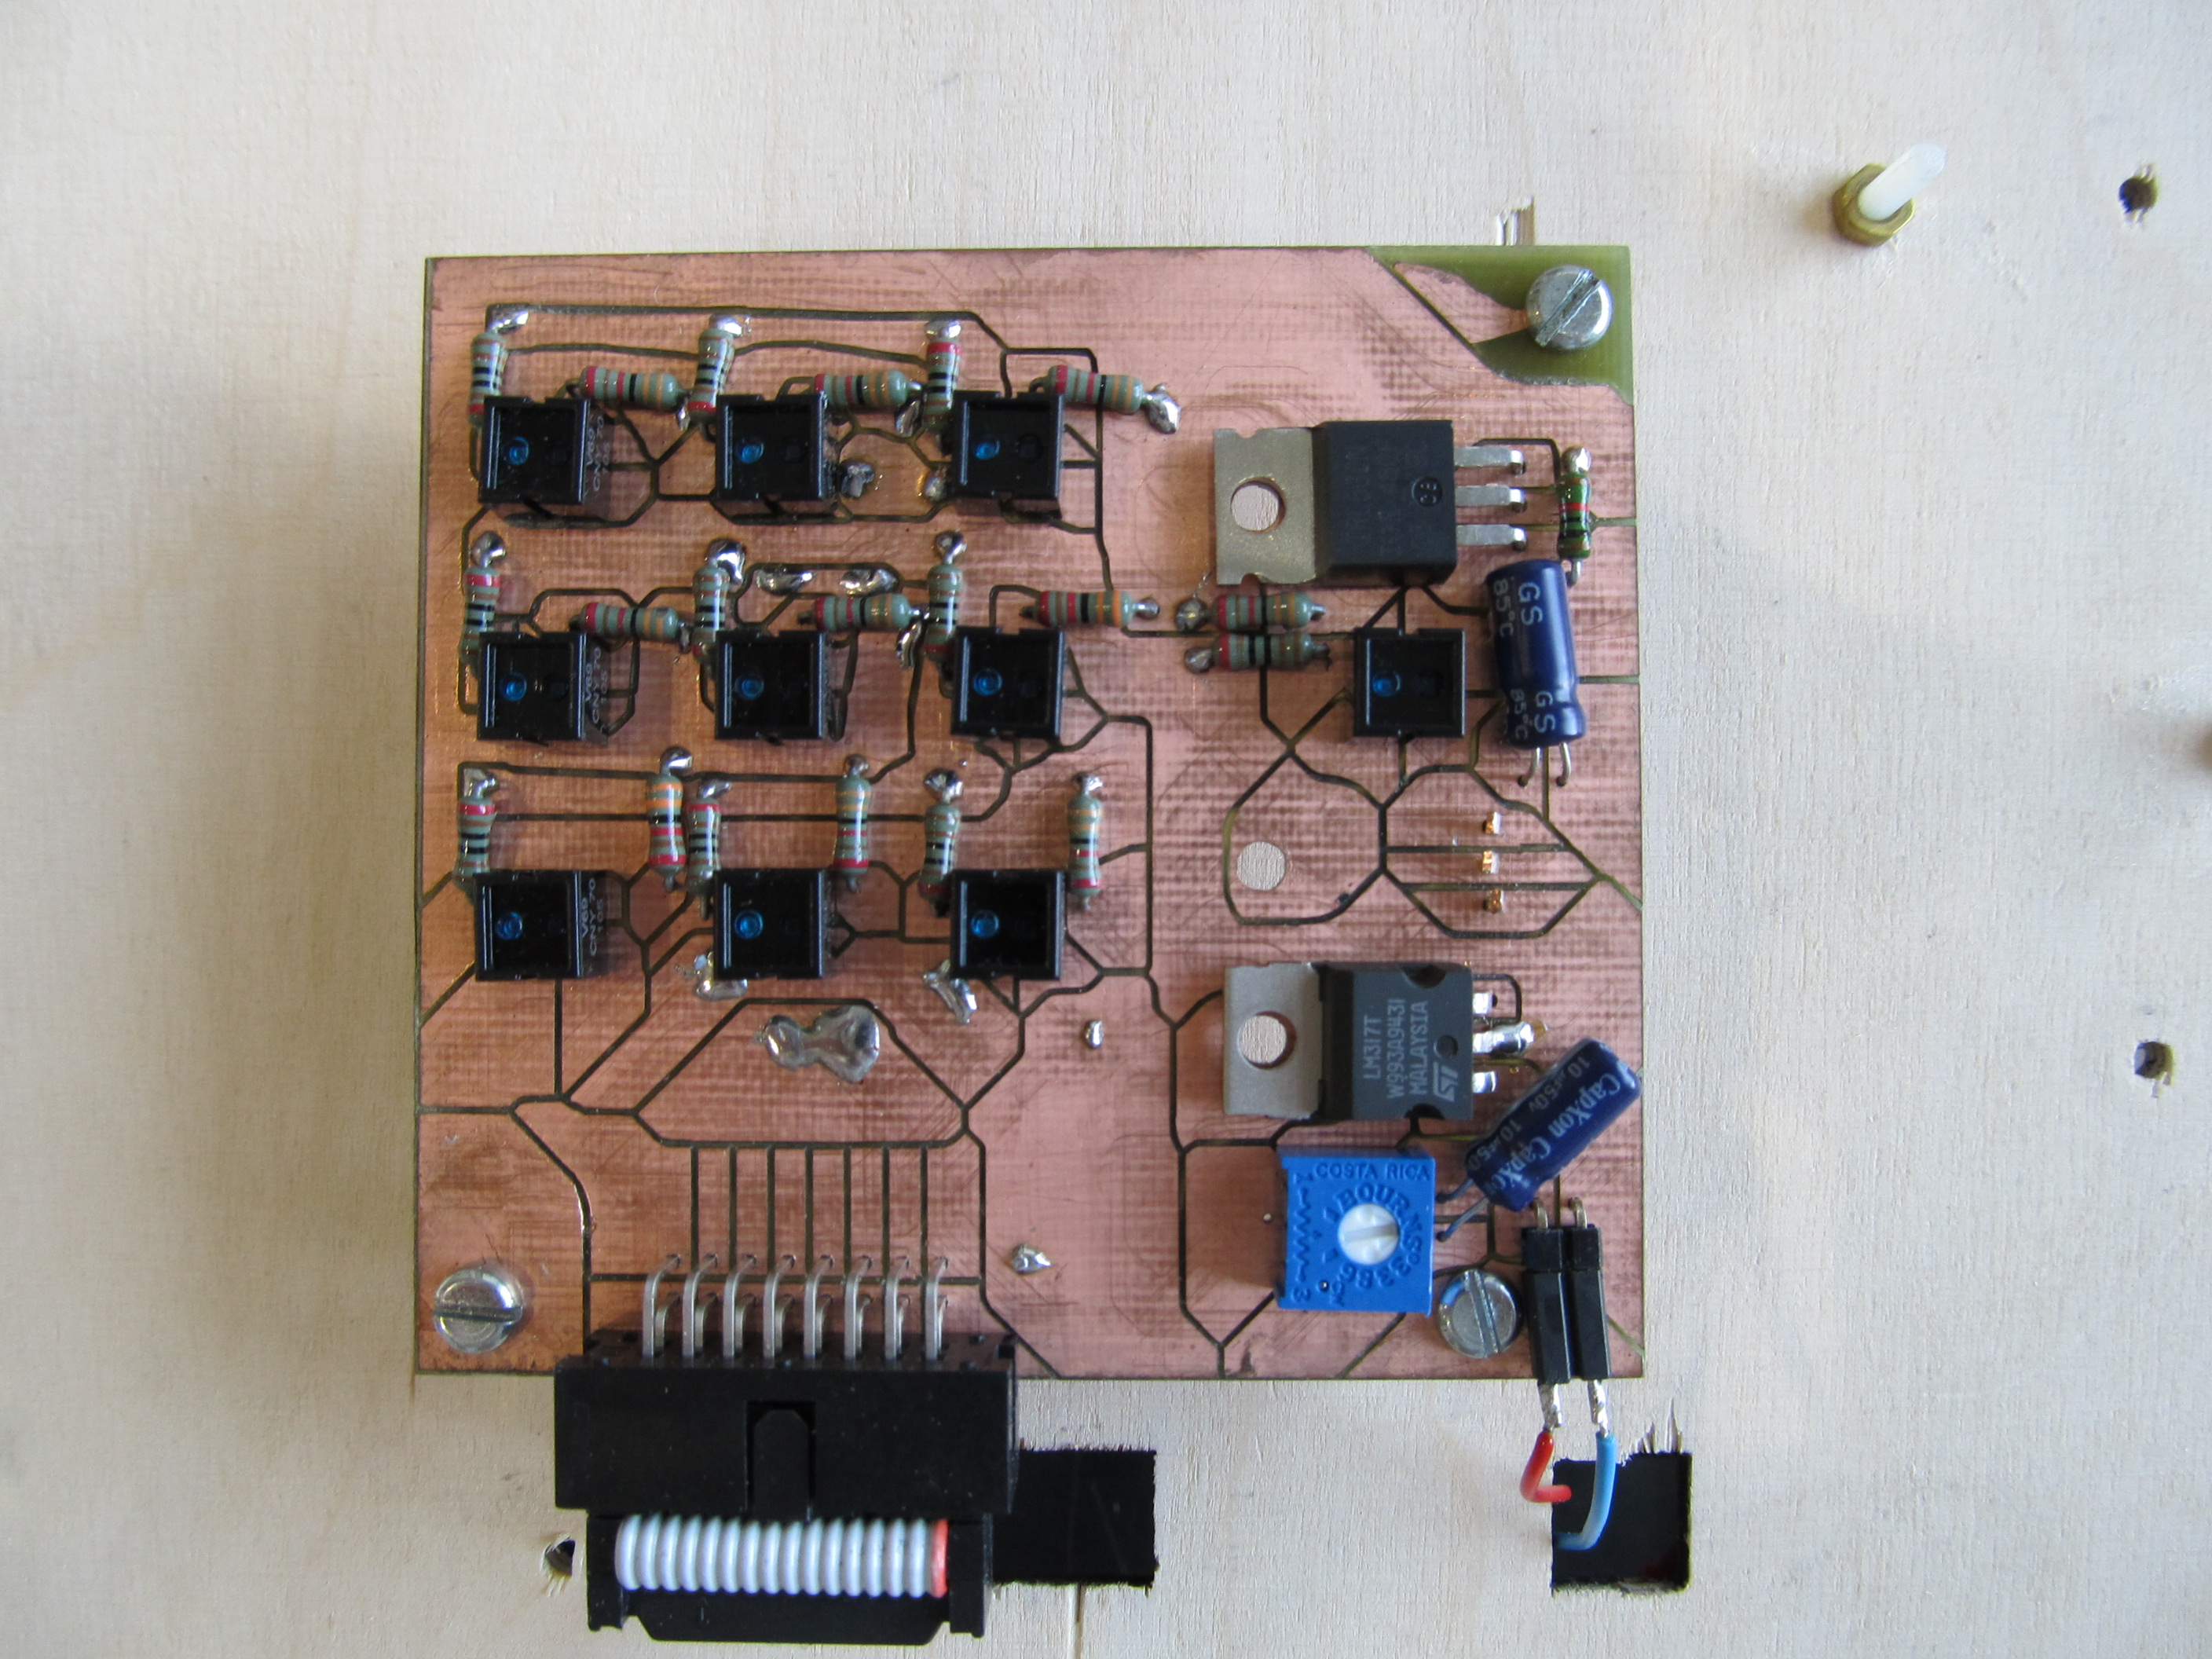
\includegraphics[width=125mm]{img/sensor_array.jpg}
\caption{Die fertige Platine des Senorarrays.}\label{array3}
\end{figure}



\subsection{Spannungversorgung}\thispagestyle{empty}
Der Roboters wird mit einem Kokam 14,8V 4000mAh Litihum Lithium-Polymer-Akkumulator, bestehend aus 4 Zellen \cite{kokam}, mit Energie versorgt. Ein voller Akku reicht für mehr mehrere Stunden Messbetrieb. Zum Laden des Akkus, was vor jedem Messzyklus empfehlenswert ist, muss der Akku vom Roboter abgesteckt werden und an das Ladegerät angeschlossen werden. Zum Schutz vor Kurzschlüssen ist der Akku mit einer im Anschlusskabel integrierten Schmelzsicherung gesichert. Da zum Laden der Akku aus dem Roboter entfernt und an das Akkuladegerät angeschlossen werden muss, könnte versehentlich der Akku kurzgeschlossen werden. Zum Laden wird ein Ultramat 16 S verwendet, der über einen Balanceranschluss verfügt, und somit alle vier Zellen des Akkus auf die gleiche Spannung lädt. 
Der Akku kann mit bis zu 200A belastet werden, allerdings liegt der maximale Strom aller 4 Motoren und der restlichen Elektronik des Roboters bei einem Ampere. Die Motoren werden direkt mit der Akkuspannung versorgt. Die Versorgungsspannung schwankt zwischen der vollen Akkuspannung 16,4V und 15V nach mehr als 10 Messfahrten.
Die 5 Volt Versorgung des Mikrocontrollers wurde mit einem RECOM R-785.0-1.0 DC-DC Konverter \cite{ref5} gelöst. Er ist pinkompatibel zu einem 7805-Spannungsregler, allerdings mit etwas größeren Ausmaßen, und bietet die Vorteile einer geringen Verlustleistung und einer sehr genauen Ausgangsspannung. 
Der Ladezustand der einzelnen Zellen des Akkus wird mit einer eigens dafür entwickelten Schaltung überwacht. Sollte die Spannung einer Zelle unter 3,3V sinken, wird die Stromversorgung zum Roboter mittels FET unterbrochen, und eine akustische Warnung ausgegeben. Damit wird eine Tiefentladung verhindert, was zu einer irreversiblen Schädigung und einem Kapazitätsverlust führen kann. Eigentlich könnte der Akku bis zu 2,7V pro Zelle entladen werden.
Die Analog-Digitalwandlung des Arduino benötigt eine Referenzspannung. Als Spannungsreferenz wird eine LT1021 5V-Präzisionsspannungsquelle \cite{lt1021} verwendet, was genauer ist als die Messsignale auf die Versorgungsspannung zu eziehen. Da dieses Bauelement nachträglich hinzugefügt wurde, ist es auf einer eigenen kleinen Platine untergebracht (siehe Abbildungen \ref{refu} und \ref{refu2}).

\begin{figure}[htbp]
\centering
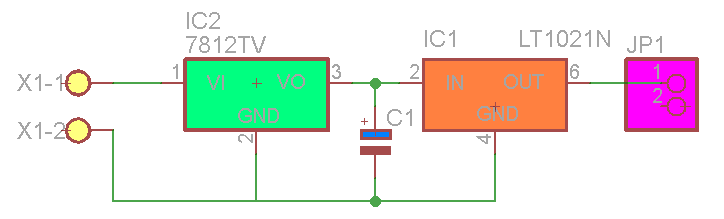
\includegraphics[width=100mm]{img/refu.png}
\caption{Die Schaltung der 5V Referenzspannung.}\label{refu}
\end{figure}

\begin{figure}[htbp]
\centering
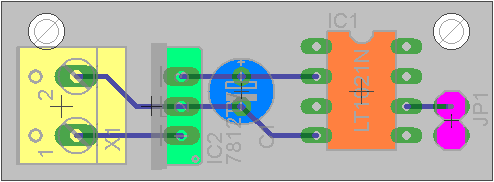
\includegraphics[width=80mm]{img/refu2.png}
\caption{Das Platinenlayout der 5V Referenzspannung.}\label{refu2}
\end{figure}

 
\subsection{Mikrokontroller}\thispagestyle{empty}
Der Arduino Mega 2560 ist eine Open-Source Elektronikentwicklungsplattform. Den Mikrocontroller des Arduino-Boards bildet ein ATmega2560 der Firma Atmel. Dabei handelt es sich um einen 8-Bit-Mikrocontroller.  Er läuft mit 16 MHz Taktfrequenz und besitzt 256 KByte Flash, wovon 8 KByte für den Bootloader verwendet werden, 8 KByte SRAM, sowie 4 KByte EEPROM.  Es verfügt über 54 digitale I/O Pins, davon können 15 als PWM-Ausgänge verwendet werden. Weiters gibt es 16 analoge Eingänge die über einen 10-Bit Analog-Digital-Wandler verfügen.
Eine USB Schnittstelle ist zur Programmierung und Kommunikation vorhanden.
Der Mikrocontroller arbeitet mit einer Versorgungsspannung von 5V.
Grundsätzlich kann die Stromversorgung über die USB Schnittstelle erfolgen. Für einen beweglichen Roboter ist diese Option jedoch nicht praktikabel. Es besteht auch die Möglichkeit über eine Buchse eine Versorgungsspannung von 7 bis 12 Volt anzulegen, der Akkumulator liefert aber eine höhere Spannung. 
Daher wird aus der Akku-Spannung mittels DC-DC Konverter eine stabile 5 Volt Spannung gewonnen. Diese 5 Volt werden direkt mit dem 5 Volt Pin des Arduino-Boards verbunden. Die 5-Volt Spannungsversorgung befindet sich auf dem Shield (der Aufsteckplatine).

\begin{figure}[htbp]
\centering
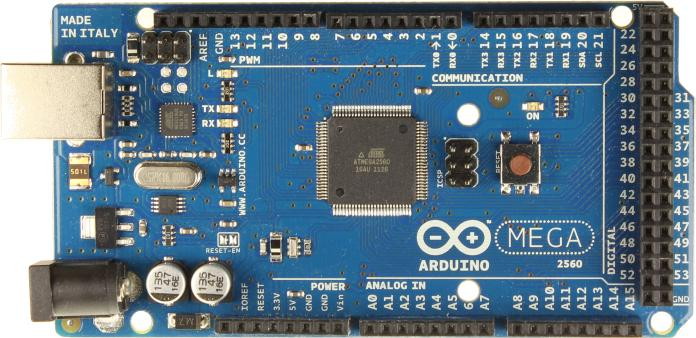
\includegraphics[width=100mm]{img/ArduinoMega2.jpg}
\caption[Arduino Mega 2560]{DAs Arduino Mega 2560 Mikrocontroller-Board.}\label{ardu}
\end{figure}

\subsection{Strommessung}\thispagestyle{empty}
Der Kurzschlussstrom der Messzelle wird mit einer eigenen Platine gemessen. Der Strom wird mittels Spannungsabfall an einem 10m$\Omega$ Shunt-Widerstand gemessen. Zu berücksichtigen ist allerdings auch der Spannungsabfall auf der Verbindung von der Zelle zum Shunt-Widerstand.
Die Zelle ist über ein 25cm langes Kabel mit dem Durchmesser von 4 mm$^2$, ein 7cm langes Kabel mit dem Durchmesser von 6mm$^2$, und zwei Bananenstecker mit der Messplatine verbunden. Der Widerstand dieser Verbindung zusammen mit dem Mess-Shunt beträgt etwa 40m$\Omega$, was bei einem Kurzschlussstrom von etwa 5 A zu einem Spannungsabfall von 200mV führt. Der gemessene Strom ist damit nicht mehr der Kurzschlussstrom. Abbildung \ref{kenn2} zeigt die Widerstandsgerade im Vergleich zur Kennlinie einer Zelle.
Als Messprinzip kommt die 4 Punktmessung zur Anwendung. 
Instrumentenverstärker: WAS IST DAS, ...

\begin{figure}[htbp]
\centering
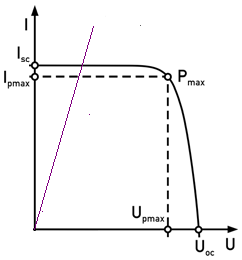
\includegraphics[width=50mm]{img/kenn2.png}
\caption{Verschiebung des Arbeitspunktes durch den Widerstand im Messpfad.}\label{kenn2}
\end{figure}

\begin{figure}[htbp]
\centering
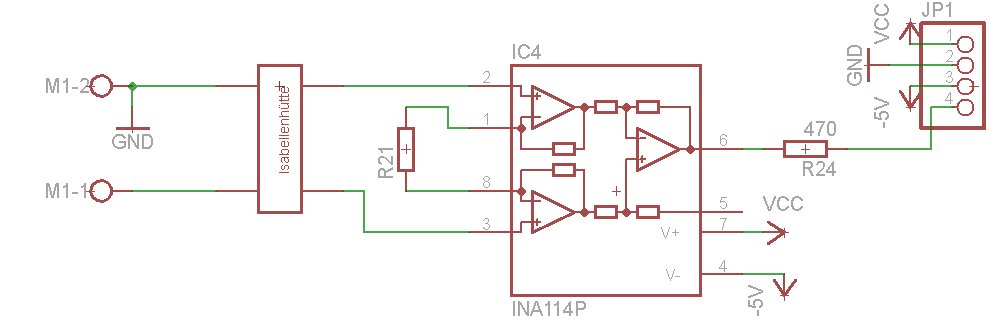
\includegraphics[width=100mm]{img/i1.png}
\caption{Die Schaltung zur Strommessung.}\label{i1}
\end{figure}

\begin{figure}[htbp]
\centering
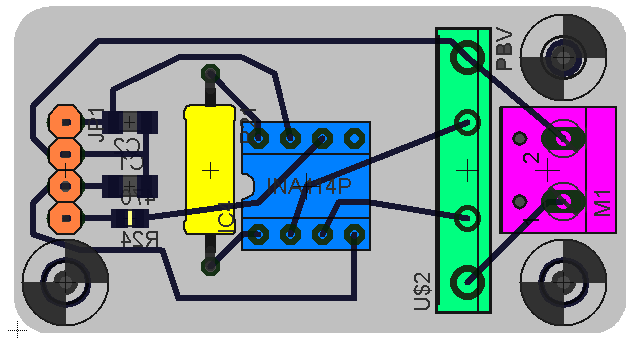
\includegraphics[width=75mm]{img/i2.png}
\caption{Die Platine zur Strommessung.}\label{i2}
\end{figure}



\subsection{Das Shield}\thispagestyle{empty}
Unter einem Shield versteht man eine Platine, die auf einem Arduino aufgesteckt werden kann, und benutzerspezifische Funktionalität beinhaltet. Im Falle des Messroboters befindet sich die Spannungsversorgung mit $\pm$5V, die SD-Karte und diverse Steckerbuchsen zum Anschluss der Messplatinen, der Motortreiberplatine und des Sensorarrays auf der Shield-Platine. 
Der SD-Karten-Connector HSR-163 \cite{hsr} benötigt eine 3,3V Versorgung, welcher der Arduino liefert. 
Zusätzlich gibt es einen TC7600-Pegelwandler \cite{tc7660}, welcher die 5V-Level der digitalen Signale des Arduino auf das für die SD-Karte notwendige 3,3V wandelt.
In der Abbildung  \ref{shield} sind die verschieden Bauteile farbig markiert:
Klemmen zur Versorgung mit Akku-Spannung (rosa), Buchse zur Kommunikation mit der Sensor-Array Platine (violett). Eine 10-polige Buchse zur Verbindung mit der Motortreiberplatine (violett). Insgesamt vier vierpolige Stecker (rosa) für verschiedene Messplatinen, wovon nur drei in Gebrauch sind: für die Strommessung und die beiden Temperaturmessungen.

\begin{figure}[htbp]
\centering
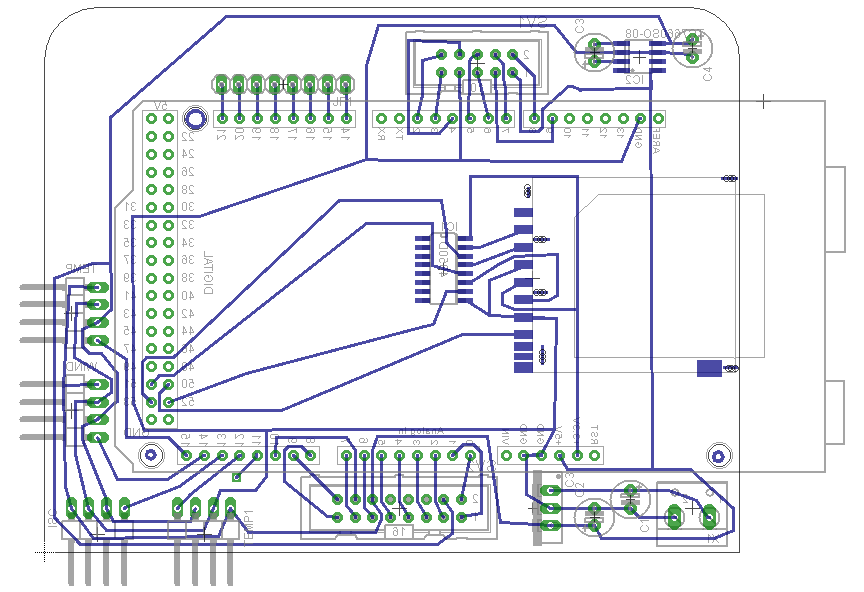
\includegraphics[width=125mm]{img/shield.png}
\caption{Die Shield-Platine.}\label{shield}
\end{figure}

\subsection{Temperaturmessung}\thispagestyle{empty}
Der Spannungsabfall an einem temperaturstabilen 100$\Omega$ Widerstand wird mit dem Spannungsabfall an einem PT100 verglichen. Durch beide Widerstände fließt ein Strom von 100$\mu$A. Als Stromquelle dient eine sehr präzise REF200-Stromquelle\cite{ref200}, welche zwei mal 100 Mikroampere $\pm$0.5$\%$ liefert. Abbildung \ref{tmess} zeigt den Schaltplan, Abbildung \ref{tmess2} zeigt das Platinenlayout. Zur besseren Idendifikation sind die Bauteile in beiden Abbildungen mit den gleichen Farben eingefärbt. 
Im Platinenlayout dient der 4-polige Stecker zur Stromversorgung (+5V, GND, -5V) und dem Abgriff des analogen Messsignales. Die 2-polige Buchse wird zum Anschluss des Temperaturmesswiderstandes verwendet.
Präzisionswiderstände wurden eingesetzt, weil sie temperaturstabiler als herkömmliche Widerstände sind. 
Die Verstärkung des INA114 berechnet sich nach \cite{ina114} wie folgt:

\begin{equation}
 G = 1 + \frac{50k\Omega}{R_G}
\end{equation} 

Aus der Abbildung \ref{pt100} erkennt man, dass der interessante Messbereich von 100 bis etwa 120$\Omega$ reicht, am Eingang des Instrumentenverstärkers liegen also maximal 2mV an, mit einer Verstärkung von 2000, wird daraus 4V, daher ist ein Widerstand von etwa 25$\Omega$ notwendig. Da es keinen solchen Präzisionswiderstand gab, wurden zwei 51,1$\Omega$ Widerstand parallel geschaltet. 

\begin{figure}[htbp]
\centering
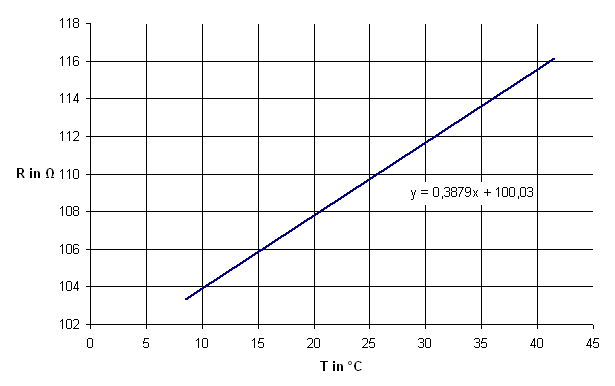
\includegraphics[width=100mm]{img/pt100.png}
\caption{Die Kennlinie eines Pt100 im Bereich von  	10$^{\circ}$C bis 40$^{\circ}$C, inklusive der linearen Näherung.}\label{pt100}
\end{figure}

\begin{figure}[htbp]
\centering
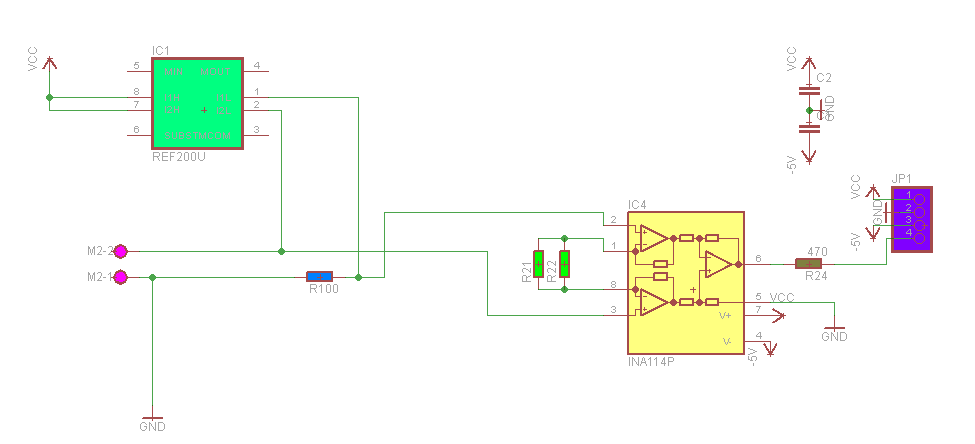
\includegraphics[width=125mm]{img/tmess.png}
\caption{Die Schaltung der Temperaturmessung.}\label{tmess}
\end{figure}

\begin{figure}[htbp]
\centering
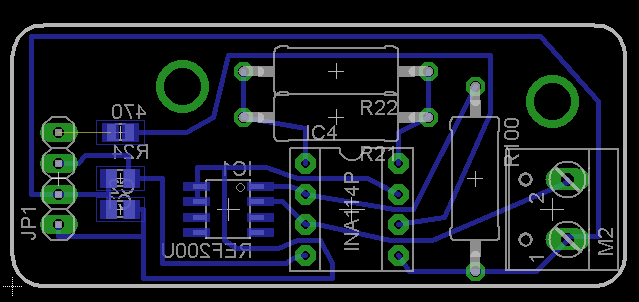
\includegraphics[width=100mm]{img/tmess2.png}
\caption{Das Layout der Temperarurmessung.}\label{tmess2}
\end{figure}






\section{Softwareentwicklung}\thispagestyle{empty}
Dieser Abschnitt beschreibt die Entwicklung der Software. Es wird kurz auf die Entwicklungsumgebung eingegangen. Dann folgt die Auswertung der optischen Sensoren. Schließlich wird die Programmstruktur erklärt. Der gesamte Code ist im Anhang gelistet.

\subsection{Entwicklungsumgebung}\thispagestyle{empty}
Der Mikrocontroller auf den Arduino Board wird mit C++ in der Arduino Entwicklungsumgebung (siehe Abbildung \ref{ardu2} programmiert, welche auf Processing basiert, programmiert. Die Entwicklungsumgebung ist auf das notwendigste beschränkt. Die vielen Beispielprogramme erlauben einen raschen Einstieg.
Ein Arduino Programm besteht aus zwei Teilen: Einer Setup-Routine die einmal zu Programmstart durchlaufen wird und einer Endlosschleife. In der Schleife wird das eigentlich Programm abgearbeitet. 

\begin{figure}[htbp]
\centering
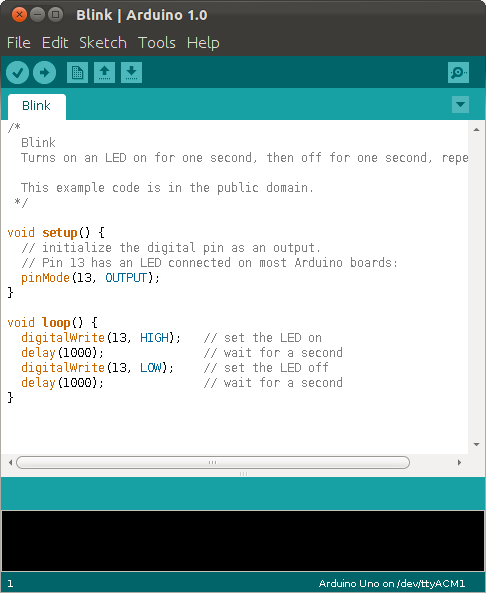
\includegraphics[width=100mm]{img/Arduino.png}
\caption{Die Arduino Entwicklungsumgebung}\label{ardu2}
\end{figure}

\subsection{Auswertung der optischen Sensoren}\thispagestyle{empty}
Um den Einfluss des Streulichtes der starken Einstrahlung im Sonnensimulator auf die Optoreflektoren CNY70 zu vermeiden, wurde eine differentielle Messmethode angewandt. Die Messwerte bei ausgeschalteter Infrarot-Leuchtdioden werden von den Messwerten mit eingeschalteter Leuchtdioden abgezogen.
Das wird für alle neun Optoreflektoren des Sensorarray, sowie den Stopsensor, gemacht.
Mit den korrigierten Werten der einzelnen optischen Sensoren wird die Lage der Linie relativ zum Mittelpunktes des Arrays bestimmt. 

Die Messwerte der optischen Sensoren ist abhängig von der Helligkeit des Untergrundes. Unter der Annahme dass sich eine gerade Linie unter dem Sensorarray befindet (siehe Abbildung \ref{arr}b), wird zuerst die Lage der Linie innerhalb einer Zeile berechnet, dazu das Extremum einer quadratischen Funktion gesucht, was der Lage der Linie innerhalb einer Zeile des Sensorarrays entspricht. 
Für alle 3 Zeilen wird so die Lage der Linie ermittelt. In diese 3 Punkte wird eine Gerade gelegt, welche die Bedingung der kleinsten Quadrate der Abstände einhält. Errechnet wird die Steigung k der Gerade, was dem Tangens der Verdrehung der Linie entspricht, und die Verschiebung d.
 
\begin{align*}
  x_1 &= \frac{C-A}{2A-4B+2C} \\
  \\
  x_2 &=  \frac{F-D}{2D-4E+2F} \\
  \\
  x_3 &=  \frac{I-G}{2G-4H+2I} \\
  \\
  d &=  \frac{x_1+x_2+x_3}{3} \\
  \\
  k &=  \frac{x_1-x_3}{2}
\end{align*}
Dabei ist es egal, ob es sich um eine helle Linie auf dunklen Untergrund, oder eine dunkle Linie auf hellem Untergrund handelt. Bei andere Teilen des Algorithmus ist das aber nicht egal. Daher funktioniert der Roboter nur mit heller Linie auf dunklen Untergrund.  Abbildung 

\begin{figure}
\centering
    \subfigure[Die Anordnung des Sensorarrays.]{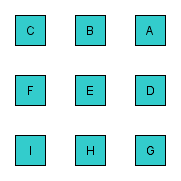
\includegraphics[width=50mm]{img/array3.png}}
    \subfigure[Die Idealposition der Linie.]{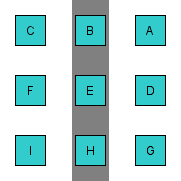
\includegraphics[width=50mm]{img/array4.png}}
\caption{Das Sensorarray.}
\label{arr}
\end{figure} 

\begin{figure}
\centering
    \subfigure[Versatz]{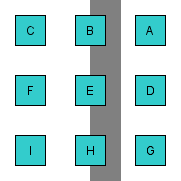
\includegraphics[width=50mm]{img/array5.png}}
    \subfigure[Verdrehung]{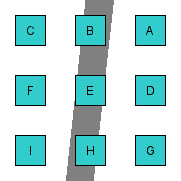
\includegraphics[width=50mm]{img/array6.png}}
\caption{Die mögliche Abweichungen der Linie von der Idealposition.}
\label{abw}
\end{figure} 

Abbildung \ref{arr} zeigt die Anordnung des Sensorarrays, die einzelnen Sensoren sind mit A bis I bezeichnet. Mögliche Abweichungen der Linie von der Idealposition sind in Abbildung \ref{abw}, auf der linken Seite, der zeitliche Versatz auf der rechten Seite, zu sehen.

\subsection{Auswertung der Temperatur- und Strommesswerte}\thispagestyle{empty}
Aufgrund von Rauschen der ADC-Werte, wurden alle Messwerte über 500 Einzelmessungen gemittelt. Die Quelle des Rauschens wurde nicht ermittelt. Der notwendige Messzeit dafür beträgt unter einer halben Sekunde. Ohne Mittelung des Messwerte schwankten die Messungen $\pm$5 Werte des ADC, das sind $\pm$0,5$\%$ bei maximalen Ausnützung bzw. $\pm$1$\%$ bei halber Ausnützung des ADC-Wertebereichs. Die gemittelten ADC-Werte werden direkt auf die SD-Karte in das Messfile gespeichert. Die eigentliche Auswertung erfolgt erst in einem Matlab Programm.
 
\subsection{Programmablauf}\thispagestyle{empty}


Das Steuerprogramm ist ein Zustandsautomat (siehe Abbildung \ref{abl}):
\begin{figure}[!]
\centering
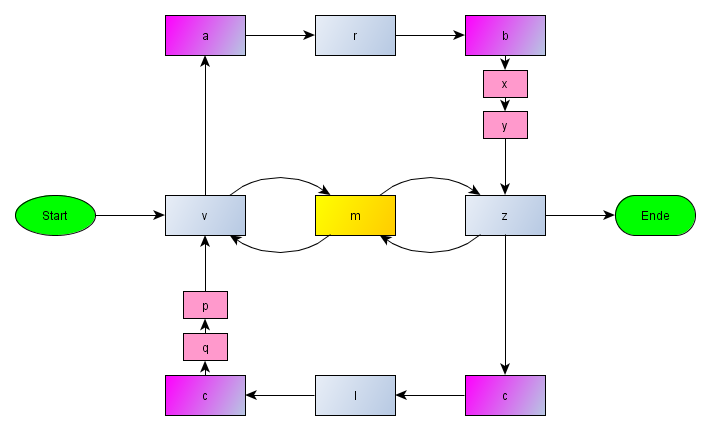
\includegraphics[width=150mm]{img/ablauf2.png}
\caption{Der Programmablauf}\label{abl}
\end{figure}
\begin{itemize}
\item Zustand \textit{s} (Start): zu Programmstart, nach 60 Sekunden Wechsel in den Zustand \textit{v}. Diese Zeitspanne dient zum schließen des Messeinschubes des Sonnensimulators nach dem Einschalten des Roboters.
\item Zustand \textit{v}: Vorwärtsfahren inklusive Regelung, Wechsel durch erkannte Ecke in den Zustand \textit{a}, bzw. durch erkannten Messpunkt Wechsel in den Zustand \textit{m}.
\item Zustand \textit{z}: Rückwärtsfahren inklusive Regelung, Wechsel bei erkannter Ecke in den Zustand \textit{c}, bzw. durch erkannten Messpunkt Wechsel in den Zustand \textit{m}.
\item Zustand \textit{m}: Messpunkt, nach Abschluss der Messung wird der bisherige Messmodus fortgesetzt.
\item Zustand \textit{r}: Rechtsfahren mit Regelung, nach erkannter Ecke Wechsel in den Zustand \textit{b}.
\item Zustand \textit{l}: Ebenfalls Rechtsfahren mit Regelung, nach erkannter Ecke Wechsel in den Zustand \textit{d}.
\item Zustand \textit{a}: Um die Ecke des Typ 1 fahren, danach Wechsel in den Zustand \textit{r}. 
\item Zustand \textit{b}: Um die Ecke des Typ 2 fahren, danach Wechsel in den Zustand \textit{x}.
\item Zustand \textit{c}: Um die Ecke des Typ 1 fahren, danach Wechsel in den Zustand \textit{l}. 
\item Zustand \textit{d}: Um die Ecke des Typ 2 fahren, danach Wechsel in den Zustand \textit{p}.
\item Zustand \textit{p}, \textit{x}: Ausrichten, danach Wechsel zu Zustand \textit{q} bzw. \textit{y}.
\item Zustand \textit{q}, \textit{y}: Ausrichten, danach Wechsel zu Zustand \textit{v} bzw. \textit{z}.
\end{itemize}

Während der Geradeaus-Fahrt wird versucht sowohl die seitliche Verschiebung d als auch die Verdrehung k zu minimieren. Wenn beide Werte innerhalb gewisser Toleranzen sind, fährt der Roboter geradeaus. Die Schranken der Regelung sind in Abbildung \ref{schr} zu sehen. Die Regelung funktioniert als Dreipunktregler für die Verdrehung, und als Dreipunktregler für die Verschiebung, wobei Verschiebung eine höhere Priorität hat als die Verdrehung. Zusätzlich gibt es noch zwei weiter Bewegungsmoden (\textbf{vtl}, \textbf{vtr}), die sich aus einer Geradeaus-Fahrt und einer überlagerten Drehung zusammensetzen, und bei nicht zu großen Verdrehungen angewendet wird.

Bei der Seitwärts-Fahrt wurde eine verbesserte Regelung angewandt, statt zwei Dreipunktreglern, wurde zwei P-Regler verwendet. Da die Motoren einen maximalen Wert für die Ansteuerung haben handelt es sich um eine Regelung mit Sättigung. Zur normalen Fahrt wird nach Rechts eine von der Verschiebung abhängige Vor/Zurück-Fahrt bzw. eine von der Verdrehung abhängige Drehung überlagert.
Abhängig von der Verschiebung d2 und der Verdrehung k2,
\begin{verbatim}
  vz = int(800*d2);
  turn = int(1600*k2);
\end{verbatim}
werden die vier Motoren (M1 bis M4) einzeln angesteuert.
\begin{verbatim}
  M1(127 + vz + turn);
  M2(-127 + vz - turn);
  M3(-127 + vz + turn);
  M4(127 + vz - turn); 
\end{verbatim}

Da die Linie für das Rechtsfahren nicht in einer Ecke endet, sondern einfach endet, kann die Regelung bis zum Ende verwendet werden. Somit entfällt ein Teil des um-die-Ecke-Fahrens. Die Faktoren des P-Regler (800, 1600) wurden durch umfangreiche Testfahrten ermittelt.

Es gibt zwei Arten von Ecken. Einmal die Ecke des Typs 1, welche eine wirkliche Ecke darstellen. Sowie die Ecke des Typs 2, welche ein eine Unterbrechung der Linie beinhaltet (siehe Abbildung \ref{ecken}).
Die beiden unterschiedlichen Arten von Ecken wurden erforderlich durch die unterschiedlichen Fahreigenschaften beim Geradeausfahren und dem Seitwärtsfahren.





\begin{figure}[htbp]
\centering
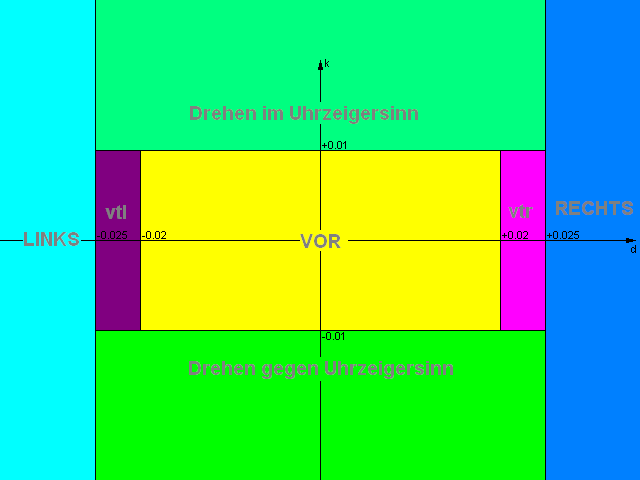
\includegraphics[width=80mm]{img/schranken.png}
\caption{Schranken der Regelung}\label{schr}
\end{figure}

\begin{figure}[htbp]
\centering
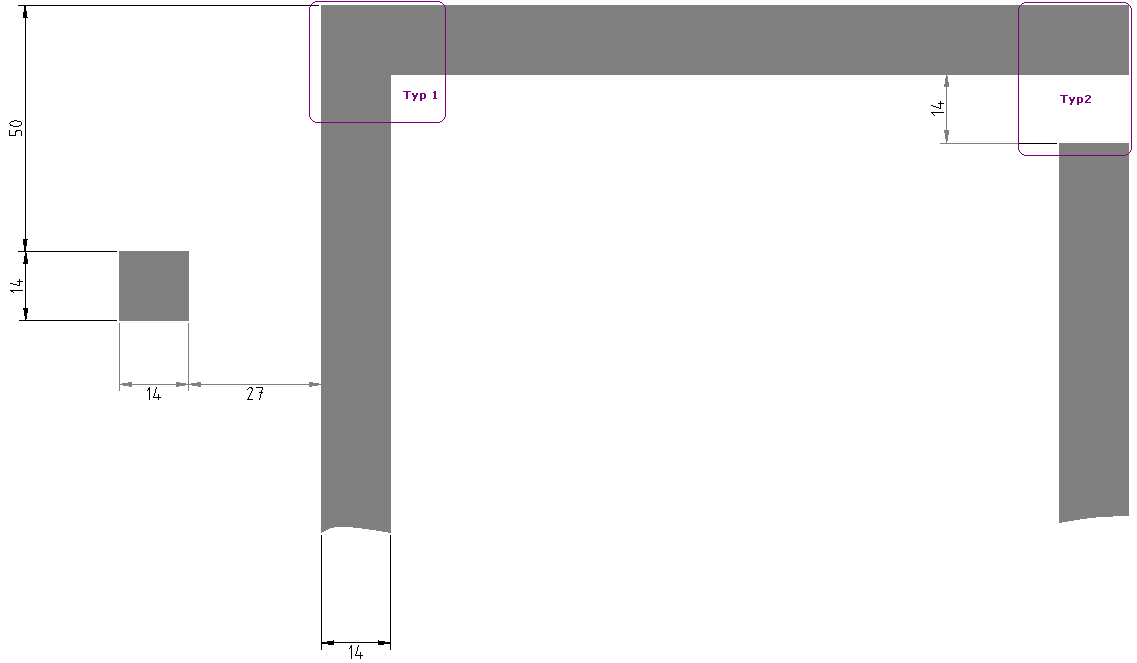
\includegraphics[width=100mm]{img/detail.png}
\caption{Eine Deatailansicht der beiden Typen von Ecken.}\label{ecken}
\end{figure}



\chapter{Kalibration}\thispagestyle{empty}

Dieses Kapitel beschreibt die Kalibrierung der Messsensoren. Es gibt drei Messplatinen, eine für die Messung des Kurzschlussstromes der Messzelle, und zwei identisch aufgebaute Messplatinen zur Messung der Zelltemperatur beziehungsweise der Umgebungstemperatur. Die Strom-Messplatine wandelt den Kurzschlussstrom der Messzelle in eine Spannung um, die in einem für den ADC des Arduino auswertbaren Bereich (0 bis 5 Volt) ist. Die beiden Messschaltungen zur Temperaturmessung wandeln die Größe der temperaturabhängigen Messwiderstände, jeweils ein Pt-100, in eine Spannung um.
Zur Kalibrierung werden die ADC-Messwerte über die USB-Schnittstelle des Roboters ausgeben. Dazu muss der Programmwahlschalter auf \textbf{K} gestellt werden.


\section{Temperatursensoren}\thispagestyle{empty}
Die Temperatur der Messzelle wird mit einem von unten aufgeklebten flächigen Folienmesswiderstand gemessen. 
Ein zweiter Pt100, in kompakter Dünnschichtbauweise ausgeführt, misst die Temperatur der Umgebung. Beide Messskreise sind identisch aufgebaut, dennoch führen Bauteiltoleranzen zu leicht unterschiedlichen Verstärkungen.
Für die Kalibration der Temperaturmesselektronik wurden die Pt-100 Widerstände durch einen hoch genaues, einstellbares und kalibriertes Messnormal ersetzt. Der Widerstand wurde im Bereich von 100 bis 122 	$\Omega$  in 1 $\Omega$  Schritten verändert, was einer Temperatur von 0 bis 55 $^{\circ}$C entspricht. Die ADC-Werte wurden über die USB-Schnittstelle des Arduino ausgelesen. Es zeigte sich, dass die beiden Schaltungen leicht unterschiedliche Verstärkungen haben. Daher mussten jede Temperaturmessschaltung separat kalibriert werden.
Obwohl der 10-Bit ADC des Arduino einen Maximalwert von 1023 hat, ist bedingt durch die 5V Versorgung des Instrumentenverstärkers INA114 (\cite{ina114}), der maximale ADC-Wert bei 857, was einer Spannung von 4,18V entspricht.  


\begin{table}[htbp]
\centering
\begin{tabular}{c c c}

\begin{tabular}{ | c | c | }\hline
{\bf R / $\Omega$ } & {\bf ADC Wert}\\ \hline
\hline
100 & ...\\ \hline
101 & 12\\ \hline
102 & 53\\ \hline
103 & 93\\ \hline
104 & 133\\ \hline
105 & 173\\ \hline
106 & 212\\ \hline
107 & 253\\ \hline
108 & 293\\ \hline
109 & 332\\ \hline
110 & 374\\ \hline
111 & 412\\ \hline
112 & 454\\ \hline
113 & 493\\ \hline
114 & 533\\ \hline
115 & 573\\ \hline
116 & 613\\ \hline
117 & 653\\ \hline
118 & 694\\ \hline
119 & 734\\ \hline
120 & 775\\ \hline
121 & 815\\ \hline
122 & 857\\ \hline
\end{tabular}


\begin{tabular}{ | c | c | }\hline
{\bf R / $\Omega$ } & {\bf ADC Wert}\\ \hline
\hline
100 & 0\\ \hline
101 & 20\\ \hline
102 & 60\\ \hline
103 & 99\\ \hline
104 & 139\\ \hline
105 & 179\\ \hline
106 & 219\\ \hline
107 & 259\\ \hline
108 & 299\\ \hline
109 & 339\\ \hline
110 & 379\\ \hline
111 & 420\\ \hline
112 & 460\\ \hline
113 & 499\\ \hline
114 & 539\\ \hline
115 & 579\\ \hline
116 & 619\\ \hline
117 & 659\\ \hline
118 & 700\\ \hline
119 & 740\\ \hline
120 & 780\\ \hline
121 & 820\\ \hline
122 & 857\\ \hline
\end{tabular}

\end{tabular}
\caption{Die Messwerte der Kalibrierung Messschaltung A und B.}\label{TabAB}
\end{table}


\begin{figure}[htbp]
\centering
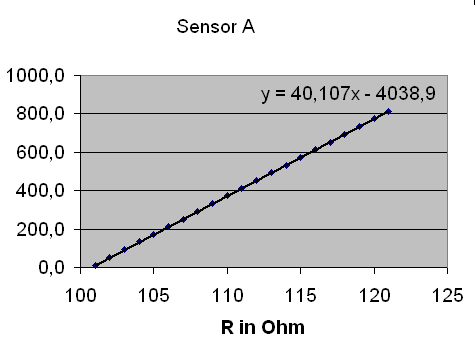
\includegraphics[width=100mm]{img/messa.png}
\caption{Die Ausgleichsgerade der Temperaturmessung A.}\label{messa}
\end{figure}


\begin{figure}[htbp]
\centering
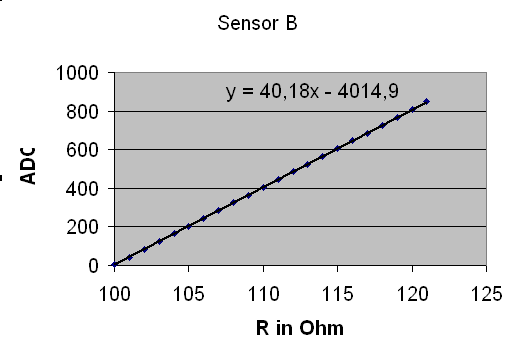
\includegraphics[width=100mm]{img/messb.png}
\caption{Die Ausgleichsgerade der Temperaturmessung B.}\label{messb}
\end{figure}

Die der Ausgleichsgerade für Messschaltung A (siehe Abbildung ~\ref{messa}) und B (siehe Abbildung ~\ref{messa}) werden verwendet um aus den ADC-Werten die dazugehörigen Widerstandswerte zu berechnen. 

  \begin{equation}
     R_A(ADC) = \frac{ADC_A + 4039,9}{40,107}
  \end{equation}
  
    \begin{equation}
     R_B(ADC) = \frac{ADC_B + 4023,6}{40,027}
  \end{equation}

 


\section{Messzelle}\thispagestyle{empty}


Der Kurzschlussstrom der Messzelle (siehe Abbildung~\ref{zelleflasher}) wurde im Flasher über einen weiten Temperaturbereich gemessen (siehe Abbildung~\ref{tempkoef}). Es wurde mit der Berger Messlast \cite{berger} gemessen. Bei der Messung wurden die Leitungswiderstände der Messkabel minimiert, indem Kabel mit hohem Querschnitt (6mm$^2$) verwendet wurden, und die Kabel möglichst kurz gehalten wurden (<1,5m).
 
\begin{figure}[htbp]
\centering
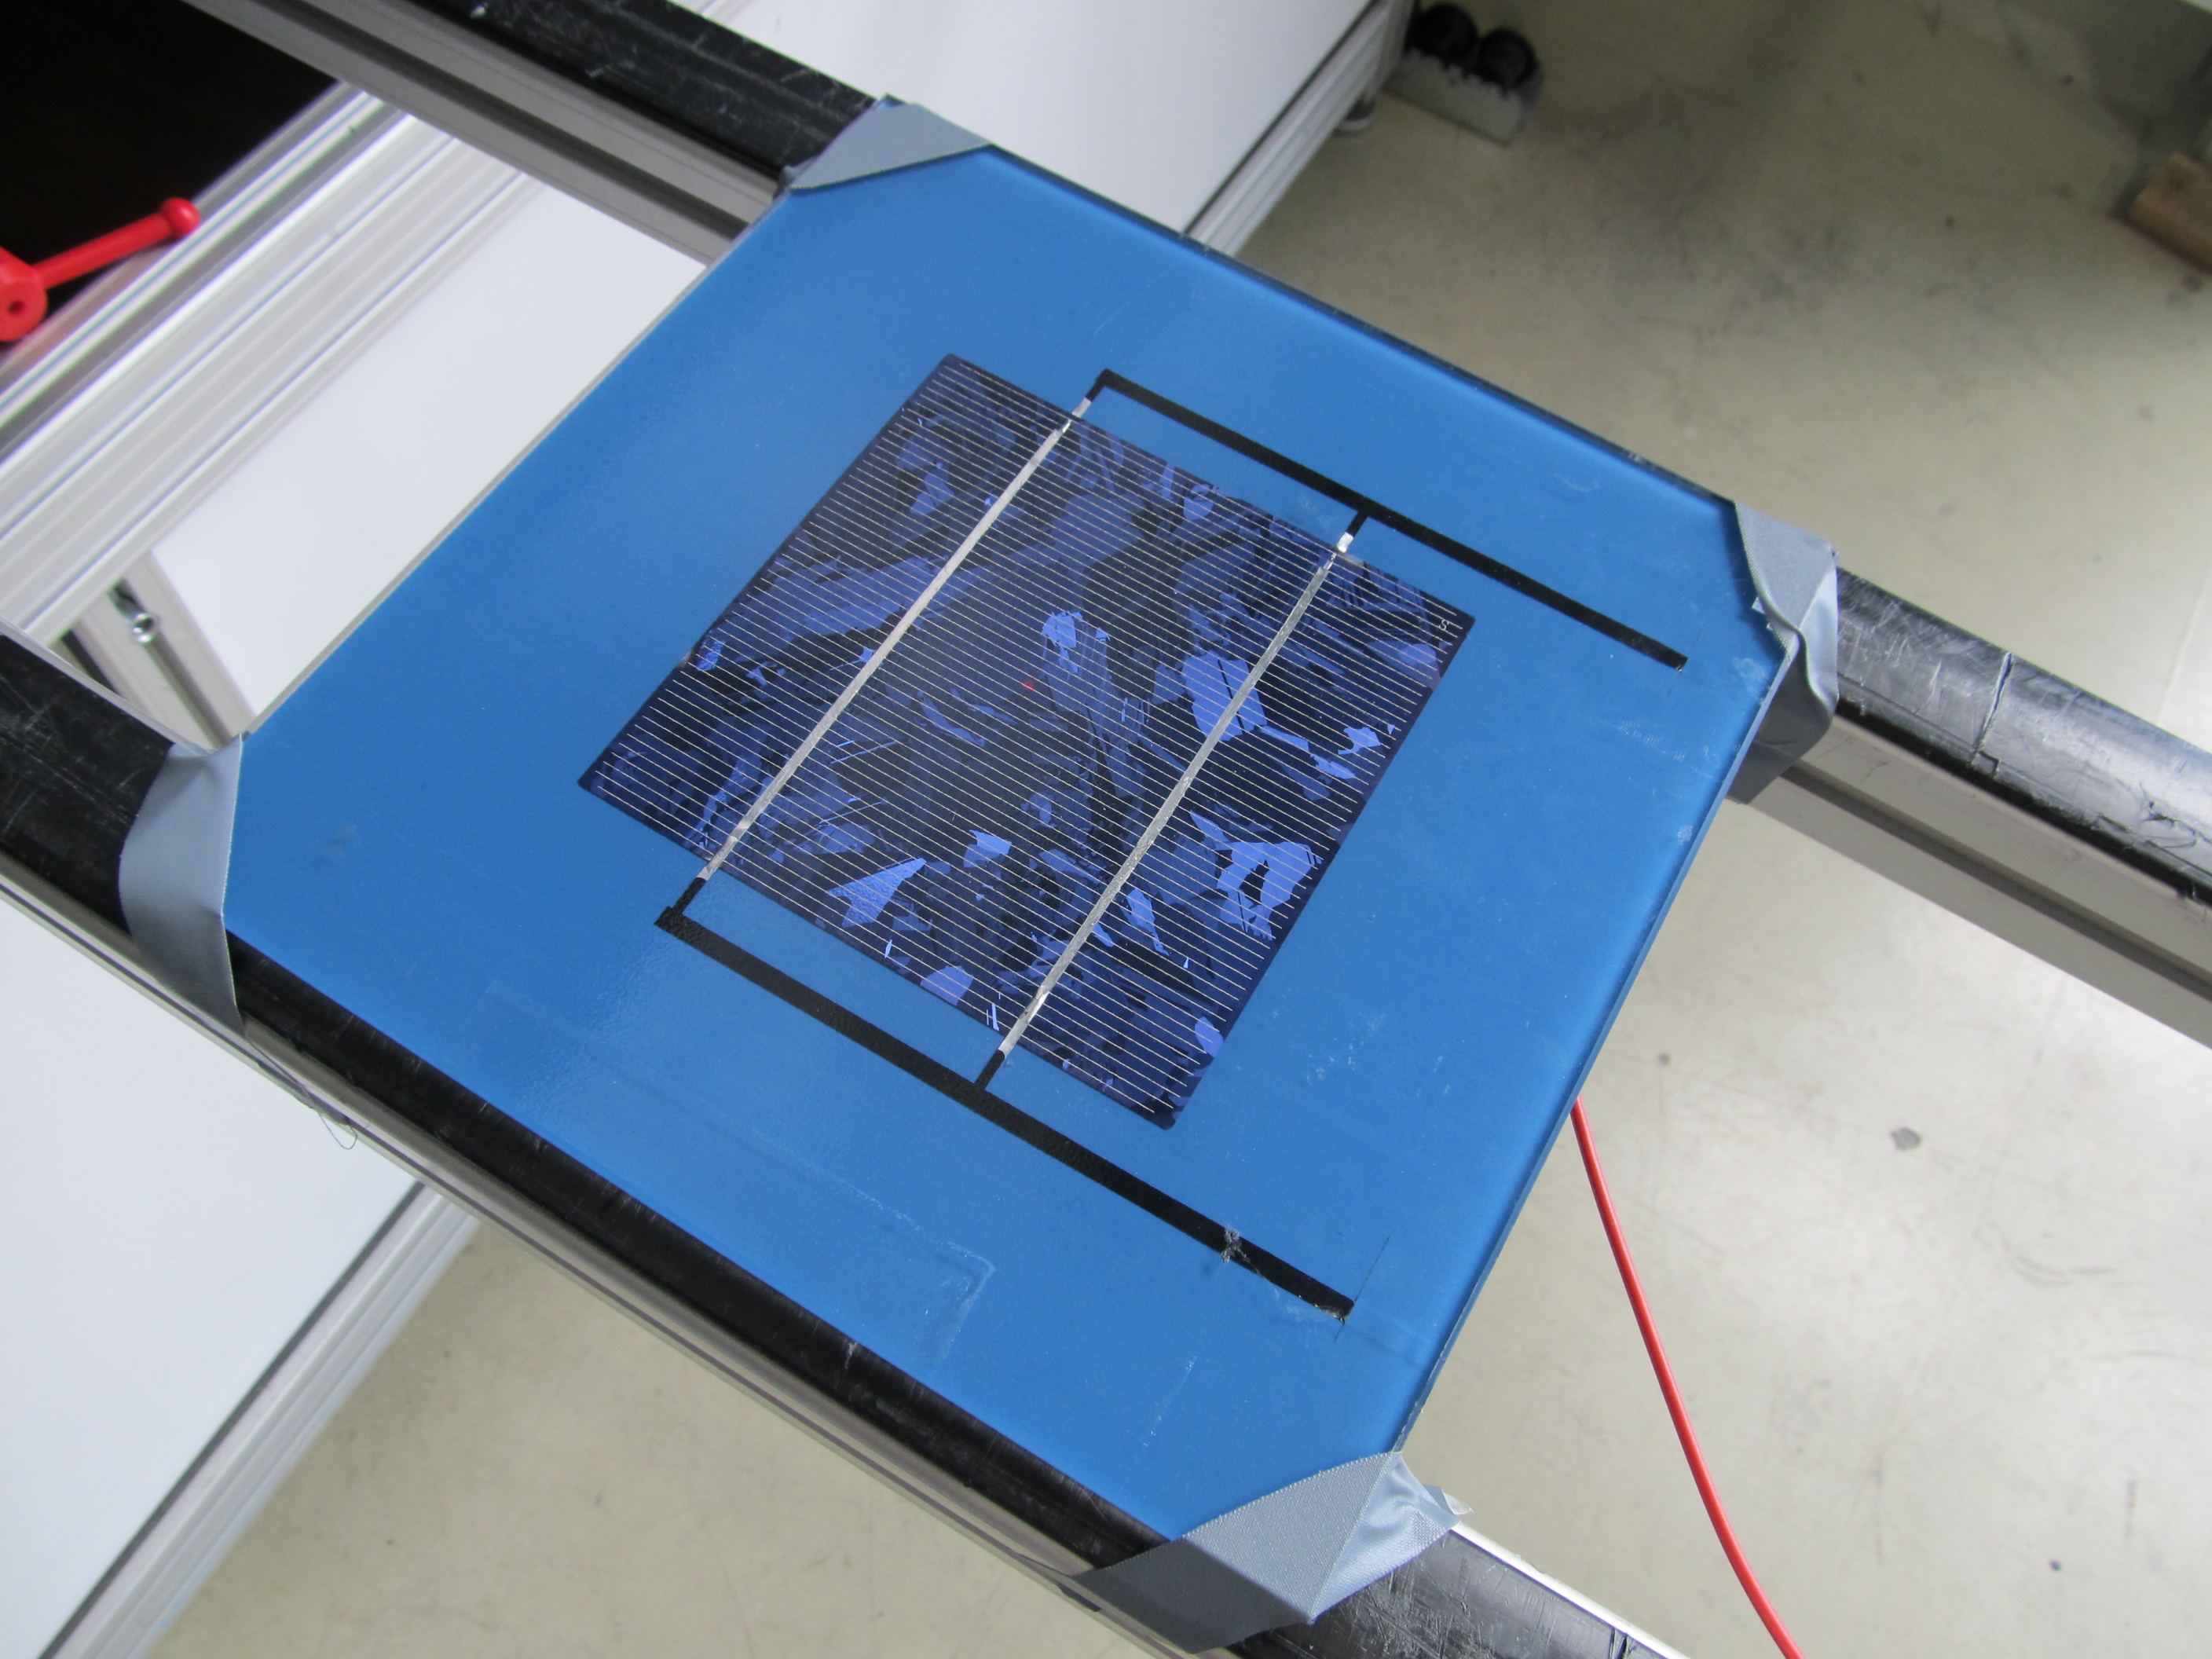
\includegraphics[width=75mm]{img/zelle.jpg}
\caption{Eine Aufnahme der Messzelle.}\label{zelleflasher}
\end{figure}

\begin{figure}[htbp]
\centering
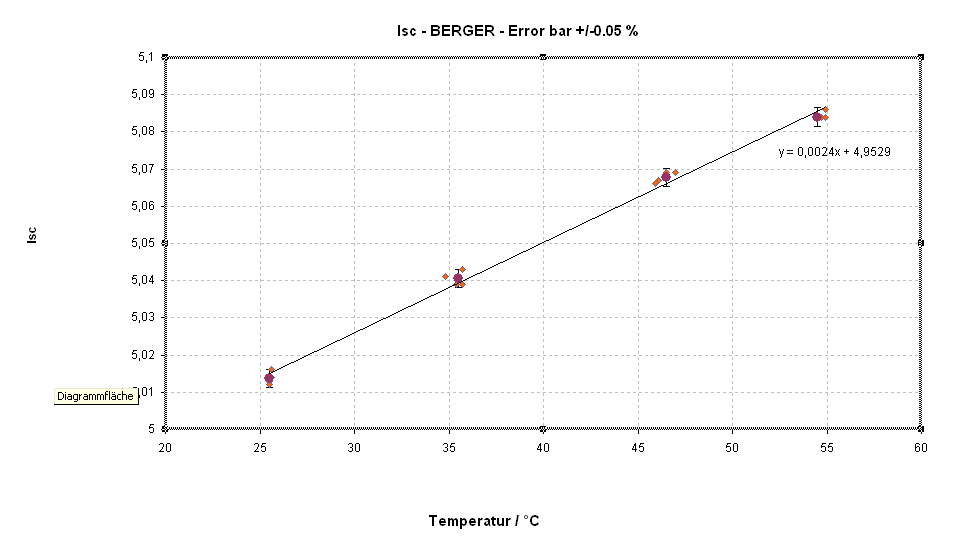
\includegraphics[width=150mm]{img/tempkoef.png}
\caption{Abhängigkeit des Kurzschlussstromes von der Temperatur.}\label{tempkoef}
\end{figure}

  \begin{equation}
     I(T) = 4,9529+0.0024 \ast T
  \end{equation}
  
    \begin{equation}
     I(T) = 4,9529 \ast ( 1 + 0,00048 \ast T)
  \end{equation}

\section{Strommessung}\thispagestyle{empty}

Der Messroboter wurde für die Kalibrierung der Kurzschlussstrommessung in eine Klimazelle platziert.  Die Temperatur der Klimazelle wurde im Bereich von 8 bis 35 $^{\circ}$C variiert. Durch den Messwiderstand der Strommessung wurde ein Strom im Bereich von 3 bis 8 A geschickt.  

\begin{table}[htbp]
\centering
\begin{tabular}{|l|l|l|}
\hline
T/$^{\circ}$C & I/mA & ADC Wert \\ 
\hline
\hline

\multirow{3}{*}{24,4} & 3997 & 472 \\
 & 6001 & 712 \\
 & 8002 & 854 \\ \hline
\multirow{3}{*}{35,3} & 3999 & 473 \\
 & 6001 & 712 \\
 & 7999 & 859 \\ \hline
\multirow{3}{*}{35,3} & 3999 & 472 \\
 & 6001 & 710 \\
 & 8001 & 852 \\ \hline
\multirow{5}{*}{16,4} & 2004 & 234 \\
 & 3005 & 353 \\
 & 4003 & 473 \\
 & 5003 & 591 \\
 & 6005 & 711 \\ \hline
\multirow{5}{*}{8} & 1993 & 233 \\
 & 2995 & 352 \\
 & 4001 & 472 \\
 & 5000 & 590 \\
 & 6005 & 710 \\ \hline
\end{tabular}
\caption{Die Kalibrierung der Strommessung}\label{TabS}
\end{table}

\begin{figure}[htbp]
\centering
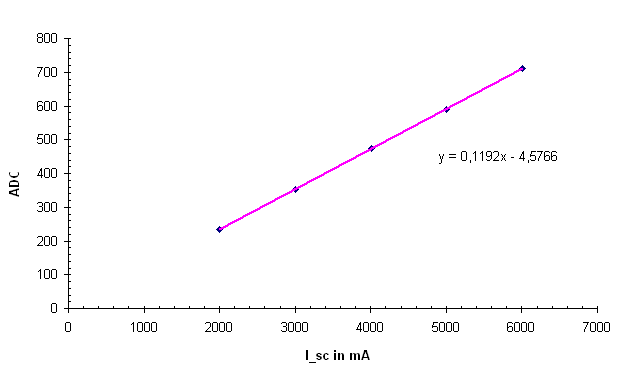
\includegraphics[width=150mm]{img/16grad.png}
\caption{Lineraer Zusammenhang zwischen Strom und dem ADC-Wert.}\label{ical}
\end{figure}

\begin{equation}
     I(ADC) = \frac{ADC + 4,5766} {119,2} 
\end{equation}
  


\section{Thermische Stabilität der Temperaturmessung}\thispagestyle{empty}
Zur Bestimmung der Temperaturstabilität wurde der gesamte Roboter in eine Klimakammer plaziert. Der Pt100 wurde durch einen temperaturstabilen 110$\Omega$ simuliert.
Beim ersten Messdurchgang zeigte sich, dass eine der beiden Messplatinen nicht temperaturstabil war (siehe Platine B in Tabelle \ref{TabT1}). Durch das Tauschen der Ref200 Stromquelle dieser Platine konnte das Problem gelöst werden. Wahrscheinlich wurde die nicht stabile Ref200-Stromquelle beim Einlöten beschädigt. Durch den Austausch der Referenzstromquelle der Platine B hat sich auch der ADC-Wert gegenüber der ersten Messung geändert. Tabelle \ref{TabT2}) zeigt die Werte nach dem Austausch.
Da die Platine A temperaturstabiler als die Platine B ist, wurde Platine A zur Messung der Zelltemperatur ausgewählt, die Platine B wurde für die Messung der Umgebungstemperatur verwendet. 

\begin{table}[htbp]
\centering
\begin{tabular}{ | c | c | c |}\hline
{\bf T / $^{\circ}$C} & {\bf ADC Platine A} & {\bf ADC Platine B}\\ \hline
\hline
11,7 & 368 & 407\\ \hline
13,0 & 368 & 406\\ \hline
13,7 & 368 & 406\\ \hline
14,5 & 368 & 405\\ \hline
15,5 & 368 & 405\\ \hline
16,6 & 368 & 405\\ \hline
17,5 & 368 & 404\\ \hline
23,5 & 368 & 403\\ \hline
27,5 & 368 & 402\\ \hline
\end{tabular}
\caption{Die Umgebungstemeraturabhängigkeit der Temperaturmessung.}\label{TabT1}
\end{table}

\begin{table}[htbp]
\centering
\begin{tabular}{ | c | c | c |}\hline
{\bf T in $^{\circ}$C} & {\bf ADC Platine A} & {\bf ADC Platine B}\\ \hline
\hline
30,7 & 368 & 380\\ \hline
20,1 & 368 & 379\\ \hline
9,2 & 368 & 378\\ \hline
\end{tabular}
\caption{Temeraturabhängigkeit der Temperaturmessung.}\label{TabT2}
\end{table}

Durch den Austausch der Referenzstromquelle der Platine B hat sich auch der ADC-Wert gegenüber der ersten Messung geändert. Die Kalibrierwerte der Platine B \ref{TabB} sind nach diesem Austausch aufgenommen worden.
Da die Platine A temperaturstabiler als die Platine B ist, wurde Platine A zur Messung der Zelltemperatur ausgewählt, die Platine B wurde für die Messung der Umgebungstemperatur verwendet. 

\chapter{Messung}\thispagestyle{empty}

Diese Kapitel beschreibt die Messvorbereitungen, den Messaufbau, die eigentliche Messungen und die Auswertung der Messdaten. Das Messsystem wurde verwendet um die Ausleuchtung der einzelnen Lampen zu ermitteln, und daraus eine für die Messebene optimierte Einstellung zu finden.

\section{Messaufbau}\thispagestyle{empty}
Die Messung der Bestrahlungsstärkeverteilung findet im Sonnensimulator statt. Zuerst muss eine Messebene geschaffen werden, auf welcher der Roboter fahren kann. Diese Fläche ist aus logistischen Gründen aus drei einzelnen Holzplatten gebildet, was zuerst einige zusätzliche Probleme bereitet hat. Auf der Oberseite der Platten befinden sich die Messpunkte und die Führungslinie, welcher der Roboter folgt. Zu Beginn der Messung wird der Roboter an das linke Ende der Linie gestellt, er fährt nach dem Einschalten selbständig das Messprogramm ab.

\begin{figure}[htbp]
\centering
\includegraphics[width=100mm]{img/robofahrt.jpg}
\caption{Eine Fahrt des Roboters auf der Messbahn.}\label{robofahrt}
\end{figure}

\subsection{Die Messebene}\thispagestyle{empty}
Die Messebene des Roboters wird von drei Holzplatten gebildet. Aus Gründen der Handhabung ist die Messebene auf drei Platten aufgeteilt. Eine einzelne 3,70 Meter mal 2,50 Meter große Platte wäre zu schwer und zu unhandlich. Die einzelnen Platten messen 250 Zentimeter mal 125 Zentimeter, und sind 18 Millimeter dick.
Die Platten sind auf der Messseite schwarz angestrichen, um die Reflexion möglichst gering zu halten. Die Messbahn sowie die Messpunkte sind weiß ausgeführt. Sowohl der schwarze Untergrund als auch die weiße Bahn besteht aus Kunstharzfarbe, welche UV-beständig und abriebfest ist. Da beim Hantieren mit den Platten dennoch kleine Beschädigungen der Messbahn entstehen können, welche den Messablauf beeinträchtigen können, so ist es sinnvoll, vor der Messung die Bahn einer optischen Kontrolle zu unterziehen und gegebenenfalls mit einem geeigneten weißen Klebeband (z.B. einem 14mm breiten Isolierband) auszubessern.
Die Platten müssen möglichst eng aneinander anliegen, damit der Roboter beim Übergang von einer Platte zur nächsten möglichst wenig behindert wird. Damit keine zu groß Stufe wegen unterschiedlicher Durchbiegung der Platten entsteht sind auf der Rückseite der Holzplatten an einigen Stellen Aluminiumbleche befestigt. An der höheren Platte wurde das Blech angeschraubt, die tiefer liegende Platte liegt darauf auf. Die Bleche wurden an den Stellen mit den größten Durchhang befestigt.
Eine zu große Stufe behindert den Roboter beim Fahren, und erschwert das zuverlässige Erkennen von Messpunkten nahe der Stufe.
Die Breite aller 3 Platten ist geringer als die Breite des Einschubes des Sonnensimulators. Damit die Messungen zu verschiedenen Zeitpunkten verglichen werden können, ist die Position der Platten zum Einschub zu dokumentieren.
Die Messpunkte liegen im Raster von 15 Zentimeter. Der Abstand zwischen dem Mittelpunkt eines Messpunktes und der Mitte der Führungslinie beträgt 40,6mm. Die Messpunkte sind kleine Quadrate der Seitenlänge von 14 Millimeter. Die Messbahn ist ebenfalls 14 Millimeter breit. Die Position der Messpunkte ist auf etwa ein bis zwei Millimeter genau.
Die Messpunkte liegen im Abstand von 15 cm, damit ist auch der Abstand zwischen den Messbahnen 15 cm. Die Übergänge der Messbahn von einer Platte zur nächsten sind mit weißem Isolierband zu überbrücken. 
Da die Messzelle nicht im Zentrum des Messroboters sitzt, sondern um zwei Zentimeter ist, gilt dies auch für die Positionen der Messpunkte, die Abbildung \ref{punkte} im Vergleich zur Abbildung \ref{platten} verdeutlicht das.
Da die Messzelle eine Abmessung von 125mm mal 125mm hat ist der gesamte Messbereich etwa 12cm größer als die größten Punktabstände. Der gesamte Messbereich ist somit 207cm mal 327cm groß.

\begin{figure}[htbp]
\centering
\includegraphics[width=125mm]{img/dreiplatten10.png}
\caption{Die Lage der Messbahn auf den Platten.}\label{platten}
\end{figure}

\begin{figure}[htbp]
\centering
\includegraphics[width=125mm]{img/punkte.png}
\caption{Die Lage der Messpunkte auf den Platten. Der gesamte Messbereich ist gelb gekennzeichnet.}\label{punkte}
\end{figure}

\begin{figure}[htbp]
\centering
\includegraphics[width=75mm]{img/lampen.png}
\caption{Die Anordnung der Lampen über der Messebene.}\label{Lampen}
\end{figure}


\subsection{Messablauf}\thispagestyle{empty}
Vor der Messung ist der Ladezustand des Akkus zu messen, und gegebenenfalls nachzuladen. Der Roboter ist auf mechanische Beschädigung zu untersuchen, besonders der Zustand der Räder ist zu kontrollieren.
Vor dem Einlegen der Platten in den Einschub des Sonnensimulators sind diese auf Beschädigungen zu untersuchen. Eine Beschädigung der Messbahn ist mit einem weißen Isolierband zu überkleben. Beschädigungen des Holzes direkt neben der Messbahn sind mit schwarzer Farbe auszubessern. Beschädigung an Stellen, die nicht im Sichtfeld das Sensorarray liegen können, sind egal.
Die Platten sind in den Einschub des Sonnensimulators zu legen. Begonnen wird mit der rechten Platte. Die Übergänge der Messbahn von einer Platte zur nächsten sind mit weißem Isolierband  der Breite 14mm zu überbrücken. 
Die Startposition des Roboters ist die linke vordere Ende der Messbahn. Der Roboter muss mit dem Sensorarray auf der Messbahn stehen, das Sensorarray befindet sich in der Mitte des Roboters. Kleinere Abweichungen der Idealposition werden beim losfahren korrigiert. 
Vor der eigentlichen Messfahrt ist eine Testfahrt mit geöffneter Lade des Sonnensimulators zu empfehlen. 
Nach der bestandenen Testfahrt wird der Sonnensimulator eingeschaltet. Bis zur Messung sind 20 bis 30 Minuten zu warten, bis die Temperaturen im Simulator und das Spektrum der Lampen stabil sind. Der Roboter kann während dieser Zeit im Sonnensimulator stehen. Die Messzelle sollte allerdings abgeschattet werden, damit diese sich nicht aufheizt. 
Zum Starten wird der Ein/Aus-Schalter von 0 auf 1 umgelegt, der Programmauswahlschalter muss auf der Position M (Messen) stehen. Dadurch wird der Mikrocontroller mit Spannung versorgt. Das Programm startet. Nach einer Pause von 60 Sekunden, die zum Schließen des Sonnensimulators notwendig ist, fährt der Roboter los. Eine Messfahrt, inklusive der Wartezeit vor der Fahrt, dauert etwa 13 Minuten. Nach Ablauf dieser Zeit wird der Roboter entnommen und die Daten der SD-Karte entnommen, oder der Roboter wird auf die Startposition gestellt um weitere Messfahrten durchzuführen.


\section{Auswertung}\thispagestyle{empty}

Die Messwerte werden auf der SD-Karte als Textdatei gespeichert. Für jeden Messpunkt gibt es eine eigene Zeile in der Textdatei. Gespeichert werden Messzeit in Millisekunden, der ADC-Wert für den Kurzschlussstrom, der ADC Wert für die Zelltemperatur, der ADC Wert für die Umgebungstemperatur, und jeweils einen Zählerwert für Messpunkt, Reihe und Spalte. Die einzelnen Werte sind durch einen Tabulator getrennt, damit ist die Datei in Matlab bearbeitbar.  
Tabelle \ref{TabSD} zeigt wie die Daten auf der SD-Karte gespeichert sind. Der erste Wert ist die Zeit in Millisekunden, die seit dem Einschalten des Roboters vergangen ist. Die nächsten 3 Werte sind Werte des Analogdigitalwandlers im Bereich von Null bis 1023, diese Werte werden ohne Umrechnung direkt auf die SD-Karte gespeichert. Es sind insgesamt 308 Messpunkte, 22 Reihen mit jeweils 14 Werten.  

 
\begin{table}[htbp]
\centering
\begin{tabular}{ | c | c | c | c | c | c | c | } 
\hline
$\frac{t}{ms}$ & I$_{SC}$ & T$_{Zelle}$ & T$_{Umgebung}$ & Messpunkt & Messreihe & Messspalte \\
\hline
\hline
{165515} & {466} & {437} & {237} & {47} & {5} & {4} \\
\hline
{167523} & {479} & {437} & {235} & {48} & {6} & {4} \\
\hline
{169551} & {471} & {437} & {228} & {49} & {7} & {4} \\
\hline
\end{tabular}
\caption{Ein Ausschnitt der Messwertedatei}\label{TabSD}
\end{table}

Im Zuge der Auswertung wird ein eindimensionales Array von 308 Messwerten in ein zweidimensionales Array von 14 mal 22 Zahlen umgewandelt. Dazu wird der erste bis zum 14. Wert des eindimensionalen Arrays zur ersten Reihe des zweidimensionalen Arrays. Der 15. bis zum 28. Wert des eindimensionalen Arrays bilden die zweite Reihe des zweidimensionalen Arrays, allerdings in umgekehrter Reihenfolge. So bildet die Reihenfolge der Messwerte des zweidimensionalen Arrays die Messfahrt des Roboters ab.
\newline

\begin{equation}
\begin{pmatrix}
n_1 \\ . \\ . \\ . \\ n_{308} 
\end{pmatrix}
\Longrightarrow
\begin{pmatrix}
n_{1}  & . &.& .& n_{14} \\
n_{28} & .& .& . &n_{15}  \\
n_{29}  &. &.& .& n_{42}  \\
. &.& .& . & . \\
n_{295}  &.& .&.& n_{308} 
\end{pmatrix}
\end{equation}

Um die eindimensionalen Messdaten in ein zweidimensionales Array, das der realen Anordnung der Messpunkte entspricht, wird folgender Matlab-Code verwendet:
\begin{verbatim}
j=1; k=1; l=1;

for(i=0:307)
    if(mod(i,28)>13) k = 28- mod(i,28);
    else k = mod(i,14)+1;
    end
    B(k,l)=A(i+1);
    if(mod(i+1,14)==0) l=l+1;
    end
end
\end{verbatim}

Der ADC Wert des Kurschlussstromes wird in Ampere umgerechnet. Dazu wird die in im Abschnitt Kalibrierung gewonnene Formel verwendet.
\begin{verbatim}
A = (I +4.5766)/119.2; 
\end{verbatim}
Aus diesem Kurzschlussstrom wird die temperaturkompensierte Bestrahlungsstärke berechnet:
\begin{verbatim}
G(i,j) = 1000 * A(i,j) / 4.99 * ( 1 - 0.00048 * (TTm(i,j) - 25));
\end{verbatim}
Die Abbildungen \ref{g3d} und \ref{g3d} zeigen die gemessene Bestrahlungsstärkeverteilung.

Die Zelltemperatur \textit{TTM} wird aus den Werten der 3. Spalte des Messfiles errechnet. Diese Werte werden wie die Strommesswerte in eine zweidimensionales Array umgewandelt. Die Umrechnung geschieht in zwei Schritten. Zuerst werden die ADC Werte in den Widerstand des Pt100 umgerechnet, und daraus wird die Temperatur berechnet.

\begin{verbatim}
Rm = (Tm +4038.9)/40.107; % ADC --> Widerstand
TTm = (Rm-100.03)/0.3879; % Widerstand --> Temperatur
\end{verbatim}



\begin{figure}[htbp]
\centering
\includegraphics[width=125mm]{img/g3d.png}
\caption{Die 3D-Ansicht der Ausleuchtung.}\label{g3d}
\end{figure}

\begin{figure}[htbp]
\centering
\includegraphics[width=125mm]{img/g2d.png}
\caption{Die 2D-Ansicht der Ausleuchtung.}\label{g2d}
\end{figure}

\begin{figure} [htbp]
    \subfigure[Die Zelltemperatur.]{\includegraphics[width=0.49\textwidth]{img/tcell.png}}
    \subfigure[Die Umgebungstemperatur.]{\includegraphics[width=0.49\textwidth]{img/t2.png}}
\caption{Die Temperaturen der Zelle und der Umgebung während einer Messfahrt.}
\label{t}
\end{figure} 

\FloatBarrier


\section{Die Ausleuchtung einzelner Lampen}

Durch die geringe Messzeit eines Messvorganges, war es möglich die Verteilung der Bestrahlungsstärke aller einzelnen Lampen in relativ kurzer Zeit zu messen. Die Lampen wurden einzeln mit einer Lampenleistung von 100\% vermessen, alle anderen Lampen waren jeweils auf 0\%. Das Lampenfeld war für alle Einzelmessungen in einer Höhe von 1870mm.
Die einzelnen Messungen sind in den Abbildungen \ref{E1} bis \ref{E10} abgebildet.
Die rechnerische Kombination aller zehn Lampen ist in Abbildung \ref{b100} zu sehen, im Vergleich dazu in Abbildung \ref{m100} die gemessene Bestrahlungsstärke aller zehn Lampen bei 100\%.
Abbildung \ref{v100} zeigt das Verhältnis der gemessenen Werte zu den berechneten. Die maximalen Abweichungen der gemessenen Werte zu den berechneten sind +0,57\% und -3,57\%, die mittlere Abweichung liegt bei -1,8\%. 

\begin{figure} [htbp]
    \subfigure[3D-Ansicht]{\includegraphics[width=0.49\textwidth]{img/E1.png}}
    \subfigure[2D-Ansicht]{\includegraphics[width=0.49\textwidth]{img/E1a.png}}
\caption{Die Ausleuchtung der Lampe E1.}
\label{E1}
\end{figure} 

\begin{figure} [htbp]
    \subfigure[3D-Ansicht]{\includegraphics[width=0.49\textwidth]{img/E2.png}}
    \subfigure[2D-Ansicht]{\includegraphics[width=0.49\textwidth]{img/E2a.png}}
\caption{Die Ausleuchtung der Lampe E2.}
\label{E2}
\end{figure} 

\begin{figure} [htbp]
    \subfigure[3D-Ansicht]{\includegraphics[width=0.49\textwidth]{img/E3.png}}
    \subfigure[2D-Ansicht]{\includegraphics[width=0.49\textwidth]{img/E3a.png}}
\caption{Die Ausleuchtung der Lampe E3.}
\label{E3}
\end{figure}

\begin{figure} [htbp]
    \subfigure[3D-Ansicht]{\includegraphics[width=0.49\textwidth]{img/E4.png}}
    \subfigure[2D-Ansicht]{\includegraphics[width=0.49\textwidth]{img/E4a.png}}
\caption{Die Ausleuchtung der Lampe E4.}
\label{E4}
\end{figure} 

\begin{figure} [htbp]
    \subfigure[3D-Ansicht]{\includegraphics[width=0.49\textwidth]{img/E5.png}}
    \subfigure[2D-Ansicht]{\includegraphics[width=0.49\textwidth]{img/E5a.png}}
\caption{Die Ausleuchtung der Lampe E5.}
\label{E5}
\end{figure} 

\begin{figure} [htbp]
    \subfigure[3D-Ansicht]{\includegraphics[width=0.49\textwidth]{img/E6.png}}
    \subfigure[2D-Ansicht]{\includegraphics[width=0.49\textwidth]{img/E6a.png}}
\caption{Die Ausleuchtung der Lampe E6.}
\label{E6}
\end{figure} 

\begin{figure} [htbp]
    \subfigure[3D-Ansicht]{\includegraphics[width=0.49\textwidth]{img/E7.png}}
    \subfigure[2D-Ansicht]{\includegraphics[width=0.49\textwidth]{img/E7a.png}}
\caption{Die Ausleuchtung der Lampe E7.}
\label{E7}
\end{figure} 

\begin{figure} [htbp]
    \subfigure[3D-Ansicht]{\includegraphics[width=0.49\textwidth]{img/E8.png}}
    \subfigure[2D-Ansicht]{\includegraphics[width=0.49\textwidth]{img/E8a.png}}
\caption{Die Ausleuchtung der Lampe E8.}
\label{E8}
\end{figure} 

\begin{figure} [htbp]
    \subfigure[3D-Ansicht]{\includegraphics[width=0.49\textwidth]{img/E9.png}}
    \subfigure[2D-Ansicht]{\includegraphics[width=0.49\textwidth]{img/E9a.png}}
\caption{Die Ausleuchtung der Lampe E9.}
\label{E9}
\end{figure} 

\begin{figure} [htbp]
    \subfigure[3D-Ansicht]{\includegraphics[width=0.49\textwidth]{img/E10.png}}
    \subfigure[2D-Ansicht]{\includegraphics[width=0.49\textwidth]{img/E10a.png}}
\caption{Die Ausleuchtung der Lampe E10.}
\label{E10}
\end{figure} 

\begin{figure} [htbp]
    \subfigure[3D-Ansicht]{\includegraphics[width=0.49\textwidth]{img/b100.png}}
    \subfigure[2D-Ansicht]{\includegraphics[width=0.49\textwidth]{img/b100k.png}}
\caption{Die Lampen E1 bis E10 100\%, berechnet aus den Einzelmessungen.}
\label{b100}
\end{figure} 

\begin{figure} [htbp]
    \subfigure[3D-Ansicht]{\includegraphics[width=0.49\textwidth]{img/m100.png}}
    \subfigure[2D-Ansicht]{\includegraphics[width=0.49\textwidth]{img/m100k.png}}
\caption{Die Lampen E1 bis E10 100\%, gemessen. }
\label{m100}
\end{figure} 

\begin{figure}[htbp]
\centering
\includegraphics[width=125mm]{img/vergleich100.png}
\caption{Vergleich der gemessenen und berechneten Verteilung}\label{v100}
\end{figure}

\FloatBarrier

\section{Variation der Lampenleistung und der Höhe des Lampenfeldes}

Es wurden die Standard-Einstellungen "Arsenal 1100W" mit einer Höhe 1870mm bzw. mit einer Höhe 4200mm verwendet. Abbildung \ref{std} zeigt die Einstellungen der einzelnen Lampen der Standardeinstellungen. Die Gesamteinstellung der Lampenleistung wurde von 96\% auf 80\% und auf 60\% verringert. Die Einstellungen der einzelnen Lampen sind in Abbildung \ref{std} dargestellt. Die Kühllufttemperatur war 15$^{\circ}$C . Von jeder Einstellung wurden zwei Messungen gemacht.

\begin{table}[htbp]
\centering
\begin{tabular}{ | c | c | c | c | c | }\hline
{\bf} & {\bf G\_{mean}} & {\bf G\_{max}} & {\bf G\_{min}} & {\bf w}\\ \hline
\hline
96\%, 1870mm & 799.0 & 899.0 & 744.3 & 9.40\\ \hline
96\%, 1870mm & 799.6 & 898.3 & 747.0 & 9.19\\ \hline
80\%, 1870mm & 618.9 & 697.2 & 577.3 & 9.40\\ \hline
80\%, 1870mm & 619.4 & 697.3 & 578.0 & 9.35\\ \hline
60\%, 1870mm & 402.4 & 449.6 & 374.7 & 9.09\\ \hline
60\%, 1870mm & 400.9 & 448.2 & 371.7 & 9.33\\ \hline
96\%, 4200mm & 468.9 & 509.5 & 410.3 & 10.78\\ \hline
96\%, 4200mm & 469.1 & 509.3 & 411.1 & 10.66\\ \hline
80\%, 4200mm & 269.2 & 395.2 & 318.9 & 10.69\\ \hline
80\%, 4200mm & 269.1 & 395.3 & 320.0 & 10.52\\ \hline
\end{tabular}
\caption{Die mittlere, maximale und minimale Einstrahlung, sowie die Nichtgleichmäßigkeit der Einstrahlung w in Abhängigkeit der Lampenparameter.}\label{TabG}
\end{table}

\begin{figure}[htbp]
\centering
\includegraphics[width=75mm]{img/std.png}
\caption{Die Standard-Einstellungen ("Arsenal 1100W") der einzelnen zehn Lampen.}\label{std}
\end{figure}


\begin{figure} [htbp]
    \subfigure[3D-Ansicht]{\includegraphics[width=0.49\textwidth]{img/st96.png}}
    \subfigure[2D-Ansicht]{\includegraphics[width=0.49\textwidth]{img/st96k.png}}
\caption{Standardeinstellungen 96\%.}
\label{st96}
\end{figure} 

\begin{figure} [htbp]
    \subfigure[3D-Ansicht]{\includegraphics[width=0.49\textwidth]{img/st80.png}}
    \subfigure[2D-Ansicht]{\includegraphics[width=0.49\textwidth]{img/st80k.png}}
\caption{Standardeinstellungen 80\%.}
\label{st80}
\end{figure} 

\begin{figure} [htbp]
    \subfigure[3D-Ansicht]{\includegraphics[width=0.49\textwidth]{img/st60.png}}
    \subfigure[2D-Ansicht]{\includegraphics[width=0.49\textwidth]{img/st60k.png}}
\caption{Standardeinstellungen 60\%.}
\label{st60}
\end{figure} 

\begin{figure} [htbp]
    \subfigure[3D-Ansicht]{\includegraphics[width=0.49\textwidth]{img/h96.png}}
    \subfigure[2D-Ansicht]{\includegraphics[width=0.49\textwidth]{img/h96k.png}}
\caption{Standardeinstellungen 96\%, Lampenfeld auf 4200mm.}
\label{h96}
\end{figure} 

\begin{figure} [htbp]
    \subfigure[3D-Ansicht]{\includegraphics[width=0.49\textwidth]{img/h80.png}}
    \subfigure[2D-Ansicht]{\includegraphics[width=0.49\textwidth]{img/h80k.png}}
\caption{Standardeinstellungen 80\%, Lampenfeld auf 4200mm.}
\label{h80}
\end{figure}

\FloatBarrier

\section{Optimierung der Homogenität}

Die Homogenität über die e Optimierungsalgorithmus: Es werden verschiedene Kombinationen der Lampeneinstellungen der zehn Lampen vorgenommen. Dabei wird das Minimum der Gleichmäßigkeit der Bestrahlungsstärkeverteilung über die Testfläche gesucht:
\begin{equation}
 Nonuniformity (\%) = [\frac{max irradiance - min irradiance}{max irradiance + min irradiance}] \times (100\%)
\end{equation}
Die beiden mittleren Lampen werden auf 100\% belassen. Die anderen Lampen werden zuerst in 3\% Schritten zwischen 80 und 100\% variiert. Dann werden, um das unter den 3\%-Schrittweiteneinstellungen gefunden Minimum, die Lampen in 1\% Schritten variiert. So werden statt der theoretisch möglichen 16,7 Billionen Möglichkeiten, nur wenige Millionen durchgerechnet, somit bleibt die Rechenzeit im Minutenbereich.

\begin{verbatim}
for k1=96:1:100
    for k2=88:1:94
        for k4=83:1:87
            for k5=92:1:100
                for k6=85:1:90
                    for k7=82:1:86
                        for k9=87:1:91
                            for k10=88:1:92
                                G = (k1*1.33-33)/100*G1 + (k2*1.33-33)/100*G2 + G3 + (k4*1.33-33)/100*G4 + 		                                    (k5*1.33-33)/100*G5 + (k6*1.33-33)/100*G6 + (k7*1.33-33)/100*G7 + G8 +  
                                    (k9*1.33-33)/100*G9 + (k10*1.33-33)/100*G10;
                                Gmin = min(min(G));
                                Gmax = max(max(G));
                                w_neu = (Gmax - Gmin)/(Gmax + Gmin) * 100;
                                if(w_neu<w)
                                    w = w_neu;
                                    K1=k1;
                                    K2=k2;
                                    K4=k4;
                                    K5=k5;
                                    K6=k6;
                                    K7=k7;
                                    K9=k9;
                                    K10=k10;                                  
                                end
                            end
                        end
                    end
                end
            end
        end
    end
end
\end{verbatim}

Mit diesem Matlab-Code wurden die in Abbildung \ref{opt} dargestellten Einstellungen gefunden.

\begin{figure}[htbp]
\centering
\includegraphics[width=75mm]{img/std.png}
\caption{Die optimierten Einstellungen der einzelnen zehn Lampen.}\label{opt}
\end{figure}

\begin{figure} [htbp]
    \subfigure[3D-Ansicht]{\includegraphics[width=0.49\textwidth]{img/optb.png}}
    \subfigure[2D-Ansicht]{\includegraphics[width=0.49\textwidth]{img/optbk.png}}
\caption{Die Berechnung der optimierten Einstellung.}
\label{optb}
\end{figure} 

\begin{figure} [htbp]
    \subfigure[3D-Ansicht]{\includegraphics[width=0.49\textwidth]{img/opt26.png}}
    \subfigure[2D-Ansicht]{\includegraphics[width=0.49\textwidth]{img/opt26k.png}}
\caption{Die Messung mit den optimierten Einstellungen.}
\label{optm}
\end{figure} 

\begin{figure}[htbp]
\centering
\includegraphics[width=125mm]{img/vergleich_opt.png}
\caption{Vergleich der gemessenen und berechneten Verteilung.}\label{v26}
\end{figure}



Das gemessene Ergebnis der optimierten Einstellung ist besser über die gesamte Ebene als die Standardeinstellungen.
Allerdings sind die Messbereiche für die Zwei-Prozentige bzw. Fünf-Prozentige Homogenität kleiner als bei den Standardeinstellungen. So macht diese Optimierung nur in Ausnahmefällen Sinn. Die Optimierung hatte die Homogenität der gesamten Ebene verbessert.

Der Suchalgorithmus für den größten Bereich, in dem die 2\% bzw. 5\% Abweichung der Homogenität gilt: Es wird für alle möglichen Teilmatrizen der Bestrahlungsstärke-Matrix die Homogenität berechnet, und so die größte gesucht, welche die 2\% bzw. die 5\% Bedingung erfüllt.
\begin{verbatim}
for m=1:13
    for n=1:21
        for k = 1:(14-m)
            for l = 1:(22-n)
                max=0;
                min=1500;
                for i = k:k+m
                    for j = l:l+n
                        if (G(i,j) > max ) max = G(i,j);
                        end
                        if (G(i,j) < min) min = G(i,j);
                        end
                        
                    end
                end
                w2 = (max - min)/(max + min) * 100;
                % Suche maximale Größe, wo die 2% bzw. 5% Schwankungsbreite
                % eingehalten wird:
                if((w2<2)&&((m+1)*(n+1)>((m2+1)*(n2+1)))&&(m>2))
                    n2 = n;
                    m2 = m;
                    k2 = k;
                    l2 = l;
                    w3 = w2;
                end
            end
        end
    end
end
\end{verbatim}

Die Abbildung \ref{zwei} zeigt den Vergleich des 2\%-Fensters zwischen den Standardeinstellungen und dem optimierten Einstellungen.
Die Abbildung \ref{funf} zeigt den Vergleich des 5\%-Fensters zwischen den Standardeinstellungen und dem optimierten Einstellungen.
In der Abbildung \ref{fstd} zeigt den 5\%-Bereich (gelb) und zwei 2\%-Bereiche (blau) mit den Standardeinstellungen.
Die 2\%- und 5\%-Bereiche der optimierten Einstellungen sind in Abbildung \ref{fopt} zu sehen. Der 5\%-Bereich mit den Standardeinstellungen größer.
In der Ausschreibung des Sonnensimulators war eine 3,4m x 2,2m bzw. 2,6m x 3m große Fläche mit einer Homogenität von 10\% respektive 5\% gefordert. 
Das Ergebnis der Validierung ist in Tballe \ref{Tab11} zu sehen. Im Vergleich dazu die Messmethode mit dem Roboter und den Standardeinstellungen des Sonnensimulators in Tabelle \ref{Tabstd}.


\begin{table}[htbp]
\centering
\begin{tabular}{ | c | c |}\hline
$\pm 10\%$ & $2,25m \times 3,45m$  \\ \hline
$\pm 5\%$ & $1,8m \times 3,15m$    \\ \hline
$\pm 2\%$ & $0,9m \times 0,6m$     \\ \hline
\end{tabular}
\caption{Validierung 2011}\label{Tab11}
\end{table}


\begin{table}[htbp]
\centering
\begin{tabular}{ | c | c |}\hline
$\pm 10\%$ & $2,07m \times 3,27m$  \\ \hline
$\pm 5\%$ & $1,77m \times 1,77m$    \\ \hline
$\pm 2\%$ & $0,87m \times 0,72m$     \\ \hline
\end{tabular}
\caption{Standardeinstellungen}\label{Tabstd}
\end{table}
Diese Methode liefert kleinere Gebiete als die Validierung im Vorjahr.

Mit den optimierten Einstellungen (Tabelle \ref{Tabopt}) sind die 2\%- und 5\%-Gebiete nochmals kleiner. Das erklärt sich dadurch, dass der Algorithmus nur die Homogenität über die gesamte Messfläche minimiert hat.
\begin{table}[htbp]
\centering
\begin{tabular}{ | c | c |}\hline
$\pm 10\%$ & $2,07m \times 3,27m$  \\ \hline
$\pm 5\%$ & $1,07m \times 2,97m$    \\ \hline
$\pm 2\%$ & $0,72m \times 0,72m$     \\ \hline
\end{tabular}
\caption{Optimierte Einstellungen}\label{Tabopt}
\end{table}

\FloatBarrier

\begin{figure}
    \subfigure[Standardeinstellungen]{\includegraphics[width=0.49\textwidth]{img/zweist.png}}
    \subfigure[Optimierte Einstellungen]{\includegraphics[width=0.49\textwidth]{img/zweiopt.png}}
\caption{Vergleich der 2\% Messbereiche}
\label{zwei}
\end{figure} 

\begin{figure}
    \subfigure[Standardeinstellungen]{\includegraphics[width=0.49\textwidth]{img/funfstd.png}}
    \subfigure[Optimierte Einstellungen]{\includegraphics[width=0.49\textwidth]{img/funfopt.png}}
\caption{Vergleich der 5\% Messbereiche}
\label{funf}
\end{figure} 

\begin{figure}[htbp]
\centering
\includegraphics[width=140mm]{img/fensterstd.png}
\caption{Die Lage der gefundenen Fenster mit den Standardeinstellungen.}\label{fstd}
\end{figure}

\begin{figure}[htbp]
\centering
\includegraphics[width=140mm]{img/fensteropt.png}
\caption{Die Lage der gefundenen Fenster mit den optimierten Einstellungen.}\label{fopt}
\end{figure}



\FloatBarrier
 
\section{Schlussfolgerung}\thispagestyle{empty}

Die Arbeit hat gezeigt, dass es möglich ist, durch ein automatisiertes Messsystem die Messzeit und den Messablauf zu verkürzen bzw. zu vereinfachen.
Prinzipiell ist diese Art von Messsystem auch für andere Sonnensimulatoren mit horizontaler Messfläche geeignet.
Aus diesen Messsystem kann eine kommerzielle Variante entwickelt werden.
Ein kommerzialisierte Variante sollte allerdings kleiner, flacher und robuster sein.
Der Roboter erleichtert die Messung der Bestrahlungsstärkeverteilung enorm. Durch die kurze Messdauer ist es möglich die Bestrahlungsstärke in periodischen Zeitabständen zu vermessen, um so die Alterung der Lampen zu dokumentieren. 
Es war möglich die Bestrahlungsstärkeverteilung aller zehn Lampen einzeln zu messen, und mit diesen Messergebnissen eine optimierte Lampeneinstellung zu finden. Eine Messung mit den optimierten Einstellungen zeigt eine hohe Übereinstimmung mit den berechneten Werten. 
Diese Art von Messroboter kann in jedem stationären Sonnensimulator entsprechender Größe zur Vermessung der Bestrahlungsstärkeverteilung verwendet werden. 
Die Verwendung des Messroboters erlaubt die Bestrahlungsstärkeverteilung einzelner Lampen zu ermitteln.
Ebenso die Bestrahlungsstärkeverteilung bei unterschiedlichen Höhen des Lampenfeldes.
Die 3D-Drucktechnik versprach zwar eine schnelle Entwicklung, sprich ein Rapid Prototyping, insgesamt benötigen die gedruckten Räder eine aufwendige Nachbearbeitung, damit sie überhaupt zusammengebaut werden konnten. Im Lauf des Roboterlebens sind einige Probleme bei den Rädern aufgetreten, die Klebung der Kugellager war nicht sehr dauerhaft, weiters war die Montage der Räder serviceintensiv, allerdings konnten mit einem besseren Kleber diese Probleme behoben werden.



% Literaturverzeichnis
% Das Literaturverzeichnis kann auch nach einem allf"alligen Anhang positiioniert werden (siehe "`Leitfaden f"ur Bachelor- und Diplomarbeiten"', Version 2.0, Abschnitt 2.9).

% M"oglichkeit 1: Erzeugung des Literaturverzeichnisses mit BibTeX:
% Die Quellen sind in der Datei *.bib (hier Literatur.bib) einzugeben. Danach muss diese Vorlage einmal geTeXt werden, dann BibTeX angewendet werden und 
% anschliessend nochmals zweimal geTeXt werden.
% Im Text erfolgt die Zitierung mit dem Anker-Schl"usselwort, z.B. \cite{kop05}.
\bibliographystyle{IEEEtran}
\bibliography{Literatur}

% M"oglichkeit 2: Erzeugung eines Literaturverzeichnisses ohne BibTeX:
%\begin{thebibliography}{99}
%\bibitem[kop05]{kop05}
%H.~Kopka, {\em LaTeX, Band 1: Einf"uhrung}, Pearson Studium, M"unchen, 3.~Auflage, 2005.
%\bibitem[knu98]{knu98}
%F.~Mittelbach, M.~Goossens, J.~Braams, D.~Carlisle, and Ch. Rowley, {\em The LaTeX Companion}, 
%Addison-Wesley, 2nd edition, 2004.
%\end{thebibliography}

% Abbildungsverzeichnis
\listoffigures
\addcontentsline{toc}{chapter}{Abbildungsverzeichnis} % f"ugt den Eintrag "Abbildungsverzeichnis" im Inhaltsverzeichnis hinzu
\newpage

% Tabellenverzeichnis
\listoftables 
\addcontentsline{toc}{chapter}{Tabellenverzeichnis} % f"ugt den Eintrag "Tabellenverzeichnis" im Inhaltsverzeichnis hinzu
\newpage

% Abk"urzungsverzeichnis
% Bei Verwendung der Dokumentklasse "scrartcl" ist der Befehlt \addchap{Abk"urzungsverzeichnis} durch 
% \addsec{Abk"urzungsverzeichnis} zu ersetzen
\addchap{Abk"urzungsverzeichnis}
\hspace{-17mm}\begin{tabular}{>{\raggedleft}p{0.2\linewidth} p{0.75\linewidth} p{0.1\linewidth}}
AM & Air Mass \\
EL & Elektrolumineszenz \\
STC & Standard Test Conditions
\end{tabular}


% Anh"ange
\begin{appendix}
\chapter{Sourcecode Arduino}

\begin{verbatim}
/*
Programm zum Steuern des Sonnensimulatormessroboters
Version 1.1 
*/

#include <SD.h>

void vor(int sped);
void zuruck(int sped);
void left(int sped);
void right(int sped);
void tl(int sped);
void tr(int sped);
void ztl();
void ztr();
void vtl();
void vtr();
void halt(); 

// ADCs zum Auslesen der 3x3 Matrix
const int analogInPin0 = A9;  
const int analogInPin1 = A2;
const int analogInPin2 = A5;
const int analogInPin3 = A8;
const int analogInPin4 = A1;
const int analogInPin5 = A4;
const int analogInPin6 = A7;
const int analogInPin7 = A0;
const int analogInPin8 = A3;
const int analogInPin9 = A6;

// Ausgang zum Schalten der Infrarot-Leds
const int analogInPin10 = A10;

// button pin
int button = 21; 

// ADC für Messwerte
const int analogInPin12 = A12;
const int analogInPin13 = A13;
const int analogInPin14 = A14;
const int analogInPin15 = A15;

// Digitalausgänge zum Ansteuern der Motoren
int IN1M1 = 2;
int IN2M1 = 3;
int IN1M2 = 4;
int IN2M2 = 5;
int IN1M3 = 6;
int IN2M3 = 9;
int IN1M4 = 7;
int IN2M4 = 8;

// Sensorwerte der optischen Sensoren (beleuchtet)
int sensorValue0 = 0;        // value read from the pot
int sensorValue1 = 0;        // value read from the pot
int sensorValue2 = 0;        // value read from the pot
int sensorValue3 = 0;        // value read from the pot
int sensorValue4 = 0;        // value read from the pot
int sensorValue5 = 0;        // value read from the pot
int sensorValue6 = 0;        // value read from the pot
int sensorValue7 = 0;        // value read from the pot
int sensorValue8 = 0;        // value read from the pot
int sensorValue9 = 0;        // value read from the pot

// Sensorwerte der optischen Sensoren (unbeleuchtet)
int sensorValue0d = 0;        // value read from the pot
int sensorValue1d = 0;        // value read from the pot
int sensorValue2d = 0;        // value read from the pot
int sensorValue3d = 0;        // value read from the pot
int sensorValue4d = 0;        // value read from the pot
int sensorValue5d = 0;        // value read from the pot
int sensorValue6d = 0;        // value read from the pot
int sensorValue7d = 0;        // value read from the pot
int sensorValue8d = 0;        // value read from the pot
int sensorValue9d = 0;        // value read from the pot

// für Auswertung der opischen Sensoren
int A = 0;
int B = 0;
int C = 0;
int D = 0;
int E = 0;
int F = 0;
int G = 0;
int H = 0;
int I = 0;
int S = 0;

// Grenzwerte für hell (=white) und dunkel (=bleak)
int white = 400;
int white2 = 250;
int bleak = 100;
int bleak2 = 150;

// zur Berechnung der Lage der LInie
float x1,x2,x3,d,k;
float y1,y2,y3,d2,k2;

// einige Hilfsvariablen
char mode='s';
char richtung='v';
int _stop=0;
int vor_ein=0;
int zuruck_ein=0;

// für die Auswertung der Messwerte
long int  temp_modul = 0; 
long int temp_i=0;
long int _Isc = 0; 
long int time = 0; 

// zur Schreiben auf die SD Karte
const int chipSelect = 53;

// Zählvariable für Messpunkt, Spalte und Reihe
int count = 0;
int count2 = 0;
int row = 1;

// zur Schreiben auf die SD Karte
String dataString = "";

// notwendig für die Kommunikation mit SD Karte
void setup() {
  pinMode(A10, OUTPUT);
  pinMode(53, OUTPUT);
  Serial.begin(9600); 
  analogReference(EXTERNAL);
  SD.begin(chipSelect);
  pinMode(button, INPUT);
}

// Definiert alle möglichen Bewegungen
void zuruck(int sped)  //speed ist besetzt!
{
  analogWrite(IN1M1,0);
  analogWrite(IN2M1,sped);   
  analogWrite(IN1M2,0);
  analogWrite(IN2M2,sped); 
  analogWrite(IN1M3,0);
  analogWrite(IN2M3,sped); 
  analogWrite(IN1M4,0);
  analogWrite(IN2M4,sped);
}  

void vor(int sped)  //speed ist besetzt!
{
  analogWrite(IN1M1,sped);
  analogWrite(IN2M1,0);   
  analogWrite(IN1M2,sped);
  analogWrite(IN2M2,0); 
  analogWrite(IN1M3,sped);
  analogWrite(IN2M3,0); 
  analogWrite(IN1M4,sped);
  analogWrite(IN2M4,0);
}

void left(int sped)  //speed ist besetzt!
{
  analogWrite(IN1M1,0);
  analogWrite(IN2M1,sped);   
  analogWrite(IN1M2,sped);
  analogWrite(IN2M2,0); 
  analogWrite(IN1M3,sped);
  analogWrite(IN2M3,0); 
  analogWrite(IN1M4,0);
  analogWrite(IN2M4,sped);
}

void right(int sped)  //speed ist besetzt!
{
  analogWrite(IN1M1,sped);
  analogWrite(IN2M1,0);   
  analogWrite(IN1M2,0);
  analogWrite(IN2M2,sped); 
  analogWrite(IN1M3,0);
  analogWrite(IN2M3,sped); 
  analogWrite(IN1M4,sped);
  analogWrite(IN2M4,0);
}

void tr(int sped)
{
  analogWrite(IN1M1,sped);
  analogWrite(IN2M1,0);   
  analogWrite(IN1M2,0);
  analogWrite(IN2M2,sped); 
  analogWrite(IN1M3,sped);
  analogWrite(IN2M3,0); 
  analogWrite(IN1M4,0);
  analogWrite(IN2M4,sped);
}

void tl(int sped)
{
  analogWrite(IN1M1,0);
  analogWrite(IN2M1,sped);   
  analogWrite(IN1M2,sped);
  analogWrite(IN2M2,0); 
  analogWrite(IN1M3,0);
  analogWrite(IN2M3,sped); 
  analogWrite(IN1M4,sped);
  analogWrite(IN2M4,0);
}

void vtr()
{   
  analogWrite(IN1M1,64);
  analogWrite(IN2M1,0);   
  analogWrite(IN1M2,0);
  analogWrite(IN2M2,64); 
  analogWrite(IN1M3,128);
  analogWrite(IN2M3,0); 
  analogWrite(IN1M4,128);
  analogWrite(IN2M4,0);
}

void vtl()
{   
  analogWrite(IN1M1,0);
  analogWrite(IN2M1,64);   
  analogWrite(IN1M2,64);
  analogWrite(IN2M2,0); 
  analogWrite(IN1M3,128);
  analogWrite(IN2M3,0); 
  analogWrite(IN1M4,128);
  analogWrite(IN2M4,0);
}

void ztr()  //speed ist besetzt!
{
  analogWrite(IN1M1,0);
  analogWrite(IN2M1,64);   
  analogWrite(IN1M2,0);
  analogWrite(IN2M2,64); 
  analogWrite(IN1M3,0);
  analogWrite(IN2M3,64); 
  analogWrite(IN1M4,64);
  analogWrite(IN2M4,0);
}  

void ztl()  //speed ist besetzt!
{
  analogWrite(IN1M1,0);
  analogWrite(IN2M1,64);   
  analogWrite(IN1M2,0);
  analogWrite(IN2M2,64); 
  analogWrite(IN1M3,64);
  analogWrite(IN2M3,0); 
  analogWrite(IN1M4,0);
  analogWrite(IN2M4,64);
}  

void halt()  //speed ist besetzt!
{
  analogWrite(IN1M1,0);
  analogWrite(IN2M1,0);   
  analogWrite(IN1M2,0);
  analogWrite(IN2M2,0); 
  analogWrite(IN1M3,0);
  analogWrite(IN2M3,0); 
  analogWrite(IN1M4,0);
  analogWrite(IN2M4,0);
}


// Hauptschleife
void loop() 
{ 
  int state = digitalRead(button);
  if (state == HIGH)
  {
    halt();

    _Isc = 0;
    temp_modul = 0;
    temp_i = 0;

    for(int i = 0; i < 500 ; i++)
    {
      _Isc = _Isc + analogRead(analogInPin13);  
      temp_modul = temp_modul + analogRead(analogInPin12); 
      temp_i = temp_i + analogRead(analogInPin15);  
      //delay(20);
    }
    _Isc = int(_Isc/500.0);
    temp_modul = int(temp_modul/500.0);
    temp_i = int(temp_i/500.0);

    Serial.print("\n I_sc = ");   
    Serial.print(_Isc);
    Serial.print("\t temp_modul = ");   
    Serial.print(temp_modul);
    Serial.print("\t temp_innen = ");   
    Serial.print(temp_i);

    delay(1000); 

  }

  else
  {

    // Werte ohne Beleuchtung:
    sensorValue0d = analogRead(analogInPin0);   
    sensorValue1d = analogRead(analogInPin1);  
    sensorValue2d = analogRead(analogInPin2);  
    sensorValue3d = analogRead(analogInPin3);  
    sensorValue4d = analogRead(analogInPin4);  
    sensorValue5d = analogRead(analogInPin5);  
    sensorValue6d = analogRead(analogInPin6);  
    sensorValue7d = analogRead(analogInPin7);  
    sensorValue8d = analogRead(analogInPin8);  
    sensorValue9d = analogRead(analogInPin9);  
    digitalWrite(A10, HIGH);  // LED ein
    delay(2); 
    // Werte mit Beleuchtung:
    sensorValue0 = analogRead(analogInPin0);   
    sensorValue1 = analogRead(analogInPin1);  
    sensorValue2 = analogRead(analogInPin2);  
    sensorValue3 = analogRead(analogInPin3);  
    sensorValue4 = analogRead(analogInPin4);  
    sensorValue5 = analogRead(analogInPin5);  
    sensorValue6 = analogRead(analogInPin6);  
    sensorValue7 = analogRead(analogInPin7);  
    sensorValue8 = analogRead(analogInPin8);  
    sensorValue9 = analogRead(analogInPin9);  
    digitalWrite(A10, LOW);

    A = sensorValue1 - sensorValue1d;
    B = sensorValue2 - sensorValue2d;
    C = sensorValue3 - sensorValue3d;
    D = sensorValue4 - sensorValue4d;
    E = sensorValue5 - sensorValue5d;
    F = sensorValue6 - sensorValue6d;
    G = sensorValue7 - sensorValue7d;
    H = sensorValue8 - sensorValue8d;
    I = sensorValue9 - sensorValue9d;

    S = sensorValue0 - sensorValue0d;

    // zum Erkennen der Linie bei vor- oder zurückfahren 
    x1 = ((C-A)/float(2*A-4*B+2*C));
    x2 = ((F-D)/float(2*D-4*E+2*F));
    x3 = ((I-G)/float(2*G-4*H+2*I));

    d = (x1 + x2 + x3)/3.; // ~ Abstand von der Ideallinie
    k = (x1-x3)/2.;  // Steigung = Verdrehung

    // zum Erkennen der Linie bei links- oder rechtsfahren
    y1 = ((G-A)/float(2*A-4*D+2*G));
    y2 = ((H-B)/float(2*B-4*E+2*H));
    y3 = ((I-C)/float(2*C-4*F+2*I));

    d2 = (y1+y2+y3)/3.;
    k2 = (y3-y1)/2.;

    if( S < bleak2) _stop=0;

    halt();

    if(E>bleak2)
    {

      switch(mode)
      {
      case 's':     // Start
        { 
          halt();
          delay(60000);  // 1 Minuten warten
          mode='v';
        }
        break;

        // Messmode
      case 'e':   // Ende
        {
          halt();
        }
        break;

      case 'm':   // Messen
        { 
          count = count + 1;  // Anzahl der Haltepunkte
          count2 = count2 + 1; 
          dataString = "";
          _stop=1;
          halt();

          delay(250);   // damit die Ströme der Fahrmotoren keinen Einfluss auf die AD-Wandlung haben

          _Isc = 0;
          temp_modul = 0;
          temp_i = 0;

          // Mittelung über jeweils 500 Messwerte
          for(int i = 0; i < 500 ; i++)
          {
            _Isc = _Isc + analogRead(analogInPin13);  
            temp_modul = temp_modul + analogRead(analogInPin12); 
            temp_i =  temp_i + analogRead(analogInPin15); 
          }
          _Isc = int(_Isc/500.0);
          temp_modul = int(temp_modul/500.0);
          temp_i = int(temp_i/500.0);
          time = millis();

          // Schreiben aud SD-Karte
          dataString += String(time);
          dataString += "\t"; 
          dataString += String(_Isc); 
          dataString += "\t"; 
          dataString += String(temp_modul); 
          dataString += "\t"; 
          dataString += String(temp_i); 
          dataString += "\t"; 
          dataString += String(count); 
          dataString += "\t"; 
          dataString += String(count2); 
          dataString += "\t"; 
          dataString += String(row); 

          // Schreibe aud SD Card
          File dataFile = SD.open("datalog.txt", FILE_WRITE);
          if (dataFile) {
            dataFile.println(dataString);
            dataFile.close();
          }

          // zurück in den Bewegungsmode
          if(richtung=='v') mode='v';
          if(richtung=='z') mode='z';

        }
        break;

      case 'v':   // Vorwärtsfahren
        { 

          richtung='v';

          if(d>0.02)  vtr();
          else 
          {  
            if(d>-0.02)  vor(128);
            else 
              vtl();
          }

          //if((C<bleak)&&(A<bleak))
          if(A<bleak2)
          {
            if(k>0.01) tr(64);
            else
            {
              if(k<-0.01) tl(64);
            }

            if(d>0.025) right(64);
            else
            {
              if(d<-0.025) left(64);
            }
          }   
          if((A>white)&&(B>white)) mode='a'; 

          if((_stop==0)&&(S>white2)) mode='m';   


        }
        break;

      case 'z': // Rückwärtsfahren
        { 

          richtung='z';

          if(d>0.02)  ztr();
          else 
          {  
            if(d>-0.02)  zuruck(128);
            else  ztl();
          }

          //if((G<bleak)&&(I<bleak))
          if(G<bleak2)
          {
            if(k>0.01) tr(64);
            else
            {
              if(k<-0.01) tl(64);
            }

            if(d>0.025) right(64);
            else
            {
              if(d<-0.025) left(64);
            }
          }
          if((G>white)&&(H>white)) mode='c';

          if((_stop==0)&&(S>white2)) mode='m';  

          if((I<bleak)&&(H<bleak)&&(G<bleak)) mode='e';

        }
        break; 

      case 'r':     //nach rechts
        {
          richtung='r';
          count2 = 0;

          right(128);
          if(D>white2)
          {
            if(d2>0.04) vor_ein=1;
            if(d2<0.02) vor_ein=0;
            if(d2<-0.04) zuruck_ein=1;
            if(d2>-0.02) zuruck_ein=0;

            if(vor_ein==1) vor(64);
            if(zuruck_ein==1) zuruck(64);

            if((vor_ein==0)&&(zuruck_ein==0))
            {
              if(k2>0.02) tr(64);
              else
              {
                if(k2<-0.02) tl(64);
              }
            }
          }

          if((D<bleak)&&(G<bleak)&&(A<bleak)) 
          { 
            mode='b';
          }

        } 
        break;

      case 'l':    // auch nach rechts 
        {
          richtung=='l';
          count2 = 0;

          right(128);
          //if((C<bleak)&&(I<bleak))
          if(D>white2)
          {
            if(d2>0.04) vor_ein=1;
            if(d2<0.02) vor_ein=0;
            if(d2<-0.04) zuruck_ein=1;
            if(d2>-0.02) zuruck_ein=0;

            if(vor_ein==1) vor(64);
            if(zuruck_ein==1) zuruck(64);

            if((vor_ein==0)&&(zuruck_ein==0))
            {
              if(k2>0.02) tr(64);
              else
              {
                if(k2<-0.02) tl(64);
              }
            }
          }

          if((D<bleak)&&(G<bleak)&&(A<bleak))
          { 
            mode='d';
          }

        } 
        break;

      case 'a':  // Um die Ecke fahren
        {
          if((A>bleak2)&&(B>bleak2)) vor(64);
          else 
          { 
            right(64);
            delay(700);
            halt();
            row = row +1 ;

            mode='r';

          }
        } 
        break; 

      case 'b':  // Um die Ecke fahren
        {

          zuruck(64);
          delay(850);
          halt();
          delay(500);

          mode='x';

        } 
        break; 

      case 'x':
        {
          if(d>0.025) right(64);

          if(d<-0.025) left(64);

          if((d<0.1)&&(d>-0.1)) mode='y';
        }
        break;

      case 'y':
        {
          if(k>0.01) tr(32);

          if(k<-0.01) tl(32);

          if((k<0.04)&&(k>-0.04)) mode='z';
        }
        break;

      case 'c':  // Um die Ecke fahren
        {
          if((H>bleak2)&&(G>bleak2 )) zuruck(64);
          else 
          { 
            right(64);
            delay(700);
            halt();
            row = row +1 ;

            mode='l';
          }
        } 
        break; 

      case 'd':  // Um die Ecke fahren
        {

          vor(64);
          delay(850);
          halt();
          delay(500);
          mode='q';

        } 
        break; 

      case 'q':
        {
          if(d>0.025) right(64);

          if(d<-0.025) left(64);

          if((d<0.1)&&(d>-0.1))       mode='p';
        }
        break;


      case 'p':
        {
          if(k>0.01) tr(32);

          if(k<-0.01) tl(32);

          if((k<0.04)&&(k>-0.04)) mode='v'; 

        }
        break;
      } 
    }   


    else 
    {  
      if((richtung=='v')||(richtung=='z'))
      {
        if((A>bleak2)||(D>bleak2)||(G>bleak2)||(C>bleak2)||(F>bleak2)||(I>bleak2))
        {
          if((A+D+G)>(C+F+I)) right(128);
          else left(128);
        }
        else halt();
      }


      if((richtung=='r')||(richtung=='l'))
      {
        if((A>bleak2)||(B>bleak2)||(C>bleak2)||(G>bleak2)||(H>bleak2)||(I>bleak2))
        {
          if((A+B+C)>(G+H+I)) vor(64);
          else zuruck(64);
        }
        else halt();
      }
    }

    delay(5); 

  }

}

\end{verbatim}

\chapter{Sourcecode Auswertung}



\begin{verbatim}

% Graphische Auswertung der Robotermesswerte

close all;
clc;
clear all;

% Öffnen der Datei, welche eine Messfahrt mit genau 308 Messwerten
% enthalten muss
fid = fopen('mess1.txt', 'r');
a = fscanf(fid, '%g %g', [7 308])     
a = a';
fclose(fid)

j=1; k=1; l=1;

% Umwandeln der 1 dimensionalen Modultemperatur ADC-Werte in eine Matrix:
for(i=0:307)
    if(mod(i,28)>13) k = 28- mod(i,28);
    else k = mod(i,14)+1;
    end
    Tm(k,l)=a(i+1,3);
    if(mod(i+1,14)==0) l=l+1;
    end
end

% Umrechnung der ADC-Werte in Temeratur:
Rm = (Tm +4038.9)/40.107;  % ADC --> Widerstand
TTm = (Rm-100.03)/0.3879;  % Widerstand --> Temperatur

j=1; k=1; l=1;

% Umwandeln der 1 dimensionalen Innentemperatur ADC-Werte in eine Matrix:
for(i=0:307)
    if(mod(i,28)>13) k = 28- mod(i,28);
    else k = mod(i,14)+1;
    end
    Ti(k,l)=a(i+1,4);
    if(mod(i+1,14)==0) l=l+1;
    end
end

% Umrechnung der ADC-Werte in Temeratur:
Ri = (Ti +4023.6)/40.027;  % ADC --> Widerstand
TTi = (Ri-100.03)/0.3879;  % Widerstand --> Temperatur

j=1; k=1; l=1;

% Umwandeln der 1 dimensionalen Kurzschlusstrom ADC-Werte in eine Matrix:
for(i=0:307)
    if(mod(i,28)>13) k = 28- mod(i,28);
    else k = mod(i,14)+1;
    end
    I(k,l)=a(i+1,2);
    if(mod(i+1,14)==0) l=l+1;
    end
end

% Umrechnung der ADC-Werte in Ampere:

A = (I +4.5766)/119.2;   % ADC --> Ampere
G_mean=0;
for i=1:14
    for j=1:22
G(i,j) = 1000 * A(i,j) / 4.99 * ( 1 - 0.00048 * (TTm(i,j) - 25));
G_mean = G_mean + G(i,j)
    end
end

G_mean = G_mean / 308;

[XI,YI] = meshgrid(1:.125:22, 1:.125:14);

Gi = interp2(G,XI,YI,'cubic'); % Interpolation

G_max = max(max(Gi));
G_min = min(min(Gi));

w = (G_max - G_min)/(G_max + G_min) * 100  % maximale Abweichung in Protzent

display(G_mean);

% Graphische Darstellung der Bestrahlungsstärke
figure;
surf(XI,YI,Gi); % in W/m2

% Bestrahlungsstärke 2D-Darstellung mit Niveaulinien
zlevs2 = 0.0:5:1000;
figure;
[C,h] = contourf(XI,YI,Gi,zlevs2);
set(h,'ShowText','on','TextStep',get(h,'LevelStep'))
colorbar;

% Graphische Darstellung der Modultemperatur
figure;
surf(TTm); 

% Graphische Darstellung der Umgebungstemperatur
figure;
surf(TTi);  

\end{verbatim} 

\end{appendix}


\end{document}
